% !TEX program = xelatex
% ============================================================
% 北京高校数学建模校际联赛 / 数学建模竞赛论文 LaTeX 模板
% 编译方式：XeLaTeX（Overleaf 中选择 XeLaTeX）
% 说明：
% 1. 本模板默认 A4 纸，四周页边距 2.5 cm。
% 2. 默认无页眉，页码位于页脚居中，从摘要页开始编号为 1。
% 3. 第一页仅放论文标题、摘要、关键词；正文从第二页开始。
% 4. 不含学校、姓名、队员编号等身份信息，请勿在正文、附录、文件名、代码路径中出现身份信息。
% 5. 正文默认宋体五号字；一级标题黑体四号，二、三级标题黑体五号。
% 6. 若赛题只有 3 问，可删除“问题四模型建立与求解”相关部分。
% ============================================================

\documentclass[UTF8,a4paper,zihao=5]{ctexart}

% ---------- 页面与字体 ----------
% 正文：宋体五号。ctex 会根据编译环境自动调用可用宋体/等价宋体；
% 在 Overleaf 或本地 TeXLive 中通常会使用 FandolSong，Windows 中通常对应 SimSun。
\AtBeginDocument{\songti\zihao{5}}
\usepackage{geometry}
\geometry{top=2.5cm,bottom=2.5cm,left=2.5cm,right=2.5cm}
\usepackage{setspace}
\setstretch{1.25}
\setlength{\parindent}{2em}
\setlength{\parskip}{0pt}

% ---------- 数学、图表、列表 ----------
\usepackage{amsmath,amssymb,amsfonts,bm,mathtools}
\usepackage{graphicx}
\usepackage{float}
\usepackage{subcaption}
\usepackage{booktabs,longtable,tabularx,array,multirow,makecell}
\usepackage{enumitem}
\usepackage{xcolor}
\usepackage{caption}
\usepackage{listings}
\usepackage{hyperref}

% ---------- 页眉页脚：不设页眉，仅页脚中部页码 ----------
\pagestyle{plain}
\pagenumbering{arabic}
\setcounter{page}{1}

% ---------- 章节格式 ----------
\ctexset{
  section = {
    name = {,、},
    number = \chinese{section},
    format = \zihao{4}\heiti\raggedright,
    beforeskip = 1.0em,
    afterskip = 0.55em
  },
  subsection = {
    format = \zihao{5}\heiti\raggedright,
    beforeskip = 0.75em,
    afterskip = 0.35em
  },
  subsubsection = {
    format = \zihao{5}\heiti\raggedright,
    beforeskip = 0.5em,
    afterskip = 0.25em
  }
}

% ---------- 图表标题 ----------
\captionsetup{font=normalsize,labelsep=space}
\numberwithin{equation}{section}
\numberwithin{figure}{section}
\numberwithin{table}{section}
\allowdisplaybreaks[4]

% ---------- 超链接 ----------
\hypersetup{
  colorlinks=true,
  linkcolor=black,
  citecolor=black,
  urlcolor=black,
  pdfauthor={},
  pdftitle={数学建模竞赛论文}
}

% ---------- 列表样式 ----------
\setlist[itemize]{leftmargin=2.2em,itemsep=0.15em,topsep=0.2em}
\setlist[enumerate]{leftmargin=2.6em,itemsep=0.15em,topsep=0.2em}

% ---------- 代码样式：若代码中包含大量中文注释，建议改用支撑文件提交，不强行全文排入正文 ----------
\lstset{
  basicstyle=\ttfamily\small,
  numbers=left,
  numberstyle=\tiny,
  frame=single,
  breaklines=true,
  columns=fullflexible,
  keepspaces=true,
  showstringspaces=false,
  tabsize=4,
  keywordstyle=\bfseries,
  xleftmargin=2em,
  framexleftmargin=1.5em
}

% ---------- 常用自定义命令 ----------
\newcommand{\diff}{\mathrm{d}}
\newcommand{\E}{\mathbb{E}}
\newcommand{\Var}{\mathrm{Var}}
\newcommand{\R}{\mathbb{R}}
\newcommand{\todo}[1]{\textcolor{red}{【待补：#1】}}

% 占位图：正式提交前请替换为 \includegraphics
\newcommand{\figplaceholder}[2]{%
\begin{figure}[H]
  \centering
  \fbox{\parbox[c][4cm][c]{0.86\linewidth}{\centering #1}}
  \caption{#2}
\end{figure}
}

\begin{document}

% ============================================================
% 第一页：标题、摘要、关键词。摘要不超过一页。
% ============================================================
\thispagestyle{plain}

\begin{center}
  {\zihao{3}\heiti 论文题目：\todo{填写完整论文题目}}\\[1.2em]
\end{center}

\noindent{\heiti 摘要}\quad
% 高分写法：摘要不是背景介绍，而是“问题—模型—结果”的压缩版。
% 建议每一问一段，每段都写清：解决什么、用什么模型、得到什么关键结果。
本文围绕\todo{题目背景与核心任务}，针对\todo{研究对象}建立了\todo{总体模型链条}，实现了\todo{预测 / 分类 / 优化 / 仿真 / 评价等目标}。全文首先对数据进行\todo{清洗、特征提取、指标构建}，随后依次建立\todo{主模型名称1、主模型名称2、主模型名称3}，并通过\todo{误差分析、交叉验证、灵敏度分析或稳定性检验}验证模型可靠性。

针对问题一，本文首先\todo{说明问题一目标}，提取\todo{核心变量或指标}，构建\todo{模型名称}。结果表明，\todo{写出最关键的数值结果、趋势或结论，不要只写“效果较好”}。

针对问题二，在问题一结果基础上，本文进一步\todo{说明问题二目标}，建立\todo{模型名称}，采用\todo{求解算法或软件}进行求解。最终得到\todo{关键结果表述，如预测值、分类准确率、最优方案、空间分布、排班方案等}。

针对问题三，考虑\todo{题目新增约束或难点，如样本不平衡、未来情景、人员扰动、环境变化等}，本文对前述模型进行改进，引入\todo{改进机制或新模型}。结果显示，\todo{关键结果与改进效果}。

若存在问题四，本文进一步\todo{说明问题四目标，如策略建议、财务评估、敏感性分析、防控方案等}，得到\todo{关键结论}。综合来看，本文模型具有\todo{准确性、解释性、鲁棒性或可操作性}，可为\todo{实际决策对象}提供定量依据。

\vspace{0.8em}
\noindent{\heiti 关键词：}\todo{关键词1}；\todo{关键词2}；\todo{关键词3}；\todo{关键词4}

\newpage

% ============================================================
% 正文：校赛可不设置目录；如确需目录，不能超过一页。
% \tableofcontents
% \newpage
% ============================================================

\section{问题重述}

\subsection{问题背景}
用自己的语言简要概括题目背景，避免大段复制题面。建议控制在 1--2 段，重点说明：研究对象是什么、现实意义是什么、为什么需要建模。

\subsection{问题要求}
按小问逐条重述，不要遗漏题目要求输出的表格、图像、编号、方案或数值。
\begin{enumerate}
  \item 问题一要求：\todo{概括问题一的输入、输出、核心目标}。
  \item 问题二要求：\todo{概括问题二的输入、输出、核心目标}。
  \item 问题三要求：\todo{概括问题三的输入、输出、核心目标}。
  \item 问题四要求：\todo{若无第四问可删除本条}。
\end{enumerate}

\section{问题分析}

% 高分写法：每一问写“目标—难点—思路—与下一问关系”。
\subsection{问题一分析}
本问的目标是\todo{目标}。主要难点在于\todo{难点，如变量关系未知、数据噪声、约束复杂、类别不平衡、时空维度高等}。因此，本文拟先\todo{数据处理或指标构建}，再建立\todo{模型}，最后通过\todo{评价方法}判断模型是否合理。本问结果将为问题二的\todo{特征、参数、约束或初始条件}提供依据。

\subsection{问题二分析}
本问在问题一的基础上，需要\todo{目标}。考虑到\todo{约束或困难}，本文采用\todo{模型或算法}，并通过\todo{验证方法}评估结果。本问的输出是\todo{必须交付的结果表或图}。

\subsection{问题三分析}
本问进一步考虑\todo{新增条件或极端情景}。本文将从\todo{模型改进、参数扰动、情景构造、类别平衡、优化约束等角度}入手，对前述模型进行扩展，最终得到\todo{结论或方案}。

\subsection{问题四分析（如有）}
本问通常对应策略建议、敏感性分析、财务评估、风险评估或推广讨论。本文拟通过\todo{检验方法或评价指标}识别关键因素，并提出\todo{可执行方案}。

\section{模型假设与符号说明}

\subsection{模型假设}
% 好的假设要解释“为什么合理”，不要只列空话。
\begin{enumerate}[label={\textbf{假设\arabic*：}}]
  \item \todo{假设内容}。\textbf{理由：}\todo{说明该假设为何符合题目背景，或对结果影响较小}。
  \item \todo{假设内容}。\textbf{理由：}\todo{说明该假设如何简化问题，以及后续是否需要灵敏度分析}。
  \item \todo{假设内容}。\textbf{理由：}\todo{说明该假设的数据依据、常识依据或文献依据}。
\end{enumerate}

\subsection{符号说明}
% 只列正文中高频、关键的符号。不要把所有临时变量都塞进表里。
\begin{longtable}{>{\centering\arraybackslash}p{0.18\linewidth}p{0.58\linewidth}>{\centering\arraybackslash}p{0.15\linewidth}}
\caption{主要符号说明}\\
\toprule
符号 & 含义 & 单位 \\
\midrule
\endfirsthead
\toprule
符号 & 含义 & 单位 \\
\midrule
\endhead
$x_i$ & \todo{决策变量或状态变量含义} & \todo{单位} \\
$y_i$ & \todo{观测值、预测值或标签含义} & \todo{单位} \\
$\theta$ & \todo{模型参数含义} & -- \\
$F$ & \todo{目标函数或评价函数} & \todo{单位} \\
$\varepsilon$ & \todo{误差项或扰动项} & -- \\
\bottomrule
\end{longtable}

\section{数据预处理与指标体系构建}

\subsection{数据来源与变量整理}
说明附件数据、自主补充数据、文献数据的来源与用途。若使用外部数据，需在参考文献中给出来源，并在附录或支撑材料中列出文件。

\begin{table}[H]
  \centering
  \caption{数据来源与用途}
  \begin{tabularx}{\linewidth}{lXX}
    \toprule
    数据名称 & 主要字段 & 用途 \\
    \midrule
    附件1 / 数据集1 & \todo{字段} & \todo{用于拟合、训练、约束或验证} \\
    附件2 / 数据集2 & \todo{字段} & \todo{用于参数估计或模型检验} \\
    外部数据 & \todo{字段} & \todo{用于补充环境变量或背景约束} \\
    \bottomrule
  \end{tabularx}
\end{table}

\subsection{数据清洗与预处理}
建议按“缺失值—异常值—重复值—单位统一—标准化/归一化—数据划分”的顺序写清楚处理规则。
\begin{enumerate}
  \item 缺失值处理：\todo{删除、插值、均值填补、模型填补等}。
  \item 异常值处理：\todo{IQR、3σ、物理阈值、人工核查等}。
  \item 数据标准化：\todo{Min-Max、Z-score、对数变换、单位换算等}。
  \item 训练与验证划分：\todo{训练集/验证集/测试集比例，或交叉验证方式}。
\end{enumerate}

\subsection{指标体系构建}
将题目中的模糊概念转化为可计算指标。例如“强度”“合理性”“非对称性”“完成度”“风险”“极端性”等。
\begin{table}[H]
  \centering
  \caption{指标体系示例}
  \begin{tabularx}{\linewidth}{lXlX}
    \toprule
    指标类别 & 指标名称 & 记号 & 计算方法 / 含义 \\
    \midrule
    规模类 & \todo{指标1} & $I_1$ & \todo{公式或解释} \\
    结构类 & \todo{指标2} & $I_2$ & \todo{公式或解释} \\
    效率类 & \todo{指标3} & $I_3$ & \todo{公式或解释} \\
    稳定类 & \todo{指标4} & $I_4$ & \todo{公式或解释} \\
    \bottomrule
  \end{tabularx}
\end{table}

\figplaceholder{此处放“全文技术路线图 / 数据处理流程图”。正式提交前替换为真实图片。}{全文技术路线图}

\section{问题一模型的建立与求解}

\subsection{模型思路}

问题一要求分析台风路径特征、强度特征与台风降水空间分布之间的关系。由于台风降水并非简单围绕台风中心对称分布，仅使用最大降水量或经纬度图难以刻画其空间结构。因此，本文从“路径--强度--环境--降水结构”的角度建立问题一模型。

具体而言，本文首先读取GPM半小时降水GeoTIFF文件，逐帧解析观测时间、台风中心位置和空间范围，并从降水栅格矩阵中提取降水强度、强降水范围、降水质心偏移、非对称性和雨带形态等指标。其次，由于CMABST路径资料时间分辨率低于GPM半小时降水资料，本文将台风路径中心、中心气压、最大风速和距岸距离等变量插值到每个GPM半小时时刻，并利用GPM文件名中给出的台风中心位置对插值结果进行误差校验。最后，本文建立Spearman相关性分析和增强随机森林解释模型，定量分析路径、强度、移动、季节和海陆因子对台风降水分布的影响。

此外，为进一步刻画台风降水相对于移动方向的空间偏向，本文不直接在经纬度坐标下分析降水场，而是建立以台风中心为原点、以台风移动方向为参考轴的台风相对运动坐标系，逐格计算前方、后方、左侧、右侧及四象限降水比例和强降水面积，从而更准确地刻画降水中心偏向、非对称性和雨带结构。

\subsection{路径数据与GPM降水数据的时间对齐}

GPM降水资料为半小时一帧，而CMABST路径资料通常不是半小时一条记录。若直接采用最近路径点匹配，会导致台风中心、强度和移动方向在半小时尺度上出现时间错位。为此，本文将路径资料插值到每一个GPM时刻。

设某场台风在路径资料中相邻两个时刻为$t_i$和$t_{i+1}$，对应的连续变量为$z_i$和$z_{i+1}$，其中$z$可表示经度、纬度、中心气压、最大风速或距岸距离等变量。对于任意GPM时刻$t\in[t_i,t_{i+1}]$，采用线性插值得到
\begin{equation}
    \hat{z}(t)=z_i+\frac{z_{i+1}-z_i}{t_{i+1}-t_i}(t-t_i).
\end{equation}

对于台风名称、编号、强度等级等离散变量，本文采用最近路径点赋值。对于经度变量，为避免跨越$180^\circ$经线时出现跳变，本文先对经度角度进行展开，再进行线性插值，最后归一化到$[-180^\circ,180^\circ]$范围内。

插值完成后，利用GPM文件名中给出的台风中心$(\lambda_t^G,\varphi_t^G)$与插值得到的路径中心$(\hat{\lambda}_t,\hat{\varphi}_t)$进行误差校验。中心误差采用Haversine球面距离：
\begin{equation}
    e_t=d_H\left((\lambda_t^G,\varphi_t^G),(\hat{\lambda}_t,\hat{\varphi}_t)\right).
\end{equation}

本文共对33420个GPM半小时时次完成路径插值匹配。校验结果如表\ref{tab:interp_quality_problem1}所示，所有样本均通过校验，中心误差均值为$0.331$ km，中位数为$0.371$ km，最大误差仅为$0.785$ km，说明插值得到的CMABST路径中心与GPM文件名中的台风中心高度一致。

\begin{table}[htbp]
    \centering
    \caption{路径插值到GPM半小时时刻后的中心误差校验}
    \label{tab:interp_quality_problem1}
    \begin{tabular}{ccccc}
        \hline
        样本数 & 正常匹配数 & 平均误差/km & 中位误差/km & 最大误差/km \\
        \hline
        33420 & 33420 & 0.331 & 0.371 & 0.785 \\
        \hline
    \end{tabular}
\end{table}

需要注意的是，GPM栅格值单位为$\mathrm{mm/hr}$，但每一帧代表半小时降水快照。因此，若某一时刻某格点降水强度为$R_t(x,y)$，则该半小时实际累计降水量为$0.5R_t(x,y)$。全过程累计降水应按
\begin{equation}
    P_{\mathrm{sum}}(x,y)=\sum_t 0.5R_t(x,y)
\end{equation}
计算。本文在问题一中主要分析半小时降水强度口径下的$R_t(x,y)$，因此$rain\_max$、$rain\_p95$等指标单位为$\mathrm{mm/hr}$；而$rain\_area\_10$表示降水强度不低于$10\ \mathrm{mm/hr}$的区域，等价于该半小时累计降水不低于$5\ \mathrm{mm}$的区域。

\subsection{降水分布特征指标体系}

设某一GPM时刻的降水强度场为$R_t(x_i,y_i)$，其中$(x_i,y_i)$为第$i$个格点的空间位置。本文从降水强度、强降水范围、降水质心偏移、固定地理方向非对称性、台风相对运动坐标系非对称性和雨带形态六个方面构建降水分布指标体系。

\subsubsection{台风中心相对坐标系}

虽然GPM降水栅格文件的空间边界已经随台风中心移动，但不同台风、不同时刻的经纬度位置不能直接用于比较降水结构。为统一刻画台风中心附近的降水空间分布，本文首先建立以台风中心为原点的局地相对坐标系。

设某一时刻台风中心经纬度为$(\lambda_c,\varphi_c)$，任一降水格点经纬度为$(\lambda,\varphi)$，则将经纬度差近似转换为以千米为单位的局地平面坐标：
\begin{equation}
    x=111\cos(\varphi_c)(\lambda-\lambda_c),
    \qquad
    y=111(\varphi-\varphi_c).
\end{equation}
其中，$x$轴正方向为正东，$y$轴正方向为正北，单位均为km。该坐标系将不同台风时刻的降水场统一到以台风中心为原点的相对空间中，便于比较降水中心偏移、降水半径和雨带形态。

\subsubsection{台风相对运动坐标系}

为了进一步分析降水结构相对于台风移动方向的前后与左右偏向，本文在台风中心相对坐标系的基础上构建台风相对运动坐标系。设台风移动方向方位角为$\alpha$，其中$\alpha=0^\circ$表示向北移动，$\alpha=90^\circ$表示向东移动，角度按顺时针方向增加。将局地坐标$(x,y)$投影到台风移动方向及其左侧法向方向，得到运动相对坐标：
\begin{equation}
    x'=x\sin\alpha+y\cos\alpha,
\end{equation}
\begin{equation}
    y'=-x\cos\alpha+y\sin\alpha.
\end{equation}

其中，$x'>0$表示格点位于台风移动前方，$x'<0$表示位于后方；$y'>0$表示位于移动方向左侧，$y'<0$表示位于右侧。由此可定义前方、后方、左侧和右侧区域：
\begin{equation}
    \Omega_F=\{(x',y'):x'>0\},\quad
    \Omega_B=\{(x',y'):x'<0\},
\end{equation}
\begin{equation}
    \Omega_L=\{(x',y'):y'>0\},\quad
    \Omega_R=\{(x',y'):y'<0\}.
\end{equation}

进一步定义四个相对运动象限：
\begin{equation}
    \Omega_{FL}=\{x'>0,y'>0\},\quad
    \Omega_{FR}=\{x'>0,y'<0\},
\end{equation}
\begin{equation}
    \Omega_{BL}=\{x'<0,y'>0\},\quad
    \Omega_{BR}=\{x'<0,y'<0\}.
\end{equation}
其中，$\Omega_{FR}$表示右前象限，$\Omega_{BL}$表示左后象限。

\subsubsection{降水强度特征}

为描述降水强度，本文计算降水场最大值、分位数和均值。重点使用最大降水强度$R_{\max}$和95分位数降水强度$R_{95}$：
\begin{equation}
    R_{\max,t}=\max_i R_t(x_i,y_i),
\end{equation}
\begin{equation}
    R_{95,t}=\mathrm{Quantile}_{0.95}\{R_t(x_i,y_i)\}.
\end{equation}
其中，$R_{\max}$反映局地极端降水峰值，$R_{95}$反映更稳定的强降水水平。

\subsubsection{强降水范围特征}

设$A_i$为第$i$个格点面积。由于GPM空间分辨率约为$0.1^\circ\times0.1^\circ$，本文按中心纬度修正格点面积：
\begin{equation}
    A_i \approx 11.1\times 11.1 \times \cos(\varphi_c)\quad(\mathrm{km^2}).
\end{equation}
定义降水强度不低于$10\ \mathrm{mm/hr}$的强降水面积为
\begin{equation}
    A_{10,t}=\sum_i A_i\mathbf{1}\{R_t(x_i,y_i)\geq 10\}.
\end{equation}
该指标等价于半小时累计降水不低于$5\ \mathrm{mm}$的区域面积。为便于解释，进一步定义强降水等效半径：
\begin{equation}
    r_{10,t}^{eq}=\sqrt{\frac{A_{10,t}}{\pi}}.
\end{equation}

\subsubsection{降水质心偏移特征}

在台风中心相对坐标系下，以降水强度为权重，定义降水质心：
\begin{equation}
    \bar{x}_t=\frac{\sum_i R_t(x_i,y_i)x_i}{\sum_i R_t(x_i,y_i)},\qquad
    \bar{y}_t=\frac{\sum_i R_t(x_i,y_i)y_i}{\sum_i R_t(x_i,y_i)}.
\end{equation}
其中，$x_i$和$y_i$分别表示第$i$个格点相对于台风中心的东西向和南北向距离，单位为km。因此，降水质心偏移距离可直接用平面距离表示为
\begin{equation}
    D_{c,t}=\sqrt{\bar{x}_t^2+\bar{y}_t^2}.
\end{equation}

若需要刻画降水质心偏移方向，则定义
\begin{equation}
    \theta_{c,t}=\operatorname{atan2}(\bar{y}_t,\bar{x}_t).
\end{equation}
其中，$\theta_{c,t}$为相对于正东方向的数学角，逆时针为正。进一步将其与台风移动方向进行比较，即可得到降水质心相对于台风运动方向的偏移角，用于判断降水中心偏向移动前方、后方、左侧或右侧。

\subsubsection{固定地理方向非对称性特征}

在台风相对坐标系下，本文首先从固定地理方向定义东西、南北非对称性。以台风中心为分界，定义东西方向非对称性：
\begin{equation}
    S_{EW,t}=
    \frac{\sum_{x_i\geq x_{c,t}}R_t(x_i,y_i)-\sum_{x_i<x_{c,t}}R_t(x_i,y_i)}
    {\sum_i R_t(x_i,y_i)}.
\end{equation}
类似地，定义南北方向非对称性：
\begin{equation}
    S_{NS,t}=
    \frac{\sum_{y_i\geq y_{c,t}}R_t(x_i,y_i)-\sum_{y_i<y_{c,t}}R_t(x_i,y_i)}
    {\sum_i R_t(x_i,y_i)}.
\end{equation}
其中，$S_{EW}>0$表示降水偏向台风中心东侧，$S_{EW}<0$表示偏向西侧；$S_{NS}>0$表示偏向北侧，$S_{NS}<0$表示偏向南侧。

\subsubsection{运动相对非对称性特征}

在台风相对运动坐标系下，以降水强度$R_i$为权重，定义前方、后方、左侧和右侧降水比例：
\begin{equation}
    Q_F=\frac{\sum_{(x'_i,y'_i)\in\Omega_F}R_i}{\sum_i R_i},
    \qquad
    Q_B=\frac{\sum_{(x'_i,y'_i)\in\Omega_B}R_i}{\sum_i R_i},
\end{equation}
\begin{equation}
    Q_L=\frac{\sum_{(x'_i,y'_i)\in\Omega_L}R_i}{\sum_i R_i},
    \qquad
    Q_R=\frac{\sum_{(x'_i,y'_i)\in\Omega_R}R_i}{\sum_i R_i}.
\end{equation}

前后非对称性和左右非对称性分别定义为：
\begin{equation}
    A_{FB}=
    \frac{
    \sum_{(x'_i,y'_i)\in\Omega_F}R_i-
    \sum_{(x'_i,y'_i)\in\Omega_B}R_i
    }{\sum_i R_i},
\end{equation}
\begin{equation}
    A_{LR}=
    \frac{
    \sum_{(x'_i,y'_i)\in\Omega_L}R_i-
    \sum_{(x'_i,y'_i)\in\Omega_R}R_i
    }{\sum_i R_i}.
\end{equation}
其中，$A_{FB}>0$表示降水偏向台风移动前方，$A_{LR}>0$表示降水偏向台风移动方向左侧。由于比例型指标分子和分母同时使用$R_i$，若改用半小时累计雨量$0.5R_i$，常数因子会同时抵消，因此不影响比例和非对称性指标的计算。

进一步地，本文还计算四象限降水比例，以及运动坐标系下前方、后方、左侧、右侧的$10\ \mathrm{mm/hr}$以上强降水面积，用于刻画强降水区相对于台风移动方向的位置。

\subsubsection{雨带形态特征}

为描述降水带是否呈狭长形态，本文将格点经纬度近似转换为以台风中心为原点的局地平面坐标，并以降水强度为权重计算二维协方差矩阵$\Sigma_t$。设$\lambda_{1,t}\geq\lambda_{2,t}$为$\Sigma_t$的两个特征值，则定义雨带各向异性指数：
\begin{equation}
    \eta_t=\frac{\sqrt{\lambda_{1,t}}-\sqrt{\lambda_{2,t}}}
    {\sqrt{\lambda_{1,t}}+\sqrt{\lambda_{2,t}}}.
\end{equation}
当$\eta_t$接近0时，降水分布接近圆形；当$\eta_t$较大时，降水带呈更明显的狭长结构。进一步地，本文计算雨带主轴方向与台风移动方向之间的夹角，用于刻画降水带相对于台风运动方向的伸展关系。

\subsection{路径、强度与环境解释变量构造}

在路径和强度特征方面，本文使用台风最大风速$V_t$、中心气压$P_t$、移动速度$U_t$、移动方向$\alpha_t$等变量。由于移动方向是周期变量，直接作为数值变量会导致$359^\circ$与$1^\circ$在数值上相差很大但实际方向接近的问题。因此，本文将移动方向转化为正弦和余弦形式：
\begin{equation}
    M_{\sin,t}=\sin\left(\frac{\pi\alpha_t}{180}\right),\qquad
    M_{\cos,t}=\cos\left(\frac{\pi\alpha_t}{180}\right).
\end{equation}

为综合描述台风强度，构造气压亏损量：
\begin{equation}
    \Delta P_t=\bar{P}-P_t,
\end{equation}
其中$\bar{P}$为样本平均中心气压。再将最大风速和气压亏损标准化，得到综合强度指数：
\begin{equation}
    I_t=\frac{1}{2}Z(V_t)+\frac{1}{2}Z(\Delta P_t).
\end{equation}
其中$Z(\cdot)$表示标准化处理。$I_t$越大，表示台风强度越强。

在海陆环境方面，使用距岸距离$d_t$、是否登陆$L_t$及近岸影响指数：
\begin{equation}
    C_t=\exp\left(-\frac{|d_t|}{200}\right).
\end{equation}
其中，$C_t$越大表示台风中心越接近海岸线，海陆热力差异、陆面摩擦和地形抬升对降水分布的调制可能越明显。

此外，为表征季节背景和日变化背景，本文构造月份和小时的周期特征：
\begin{equation}
    T_{\mathrm{month},\sin}=\sin\left(\frac{2\pi m}{12}\right),\quad
    T_{\mathrm{month},\cos}=\cos\left(\frac{2\pi m}{12}\right),
\end{equation}
\begin{equation}
    T_{\mathrm{hour},\sin}=\sin\left(\frac{2\pi h}{24}\right),\quad
    T_{\mathrm{hour},\cos}=\cos\left(\frac{2\pi h}{24}\right).
\end{equation}

综上，问题一中用于解释降水分布的主要变量包括台风强度、移动过程、强度变化率、距岸距离、近岸影响和时间背景等。主要变量如表\ref{tab:variables_problem1}所示。

\begin{table}[htbp]
    \centering
    \caption{问题一主要解释变量与响应变量}
    \label{tab:variables_problem1}
    \begin{tabular}{p{0.25\textwidth}p{0.65\textwidth}}
        \hline
        变量类别 & 具体变量 \\
        \hline
        强度变量 & 最大风速、中心气压、气压亏损、综合强度指数 \\
        移动变量 & 移动速度、移动方向正弦、移动方向余弦 \\
        演变变量 & 风速变化率、气压变化率、增强/减弱状态 \\
        海陆变量 & 是否登陆、距岸距离、有符号距岸距离、近岸影响指数 \\
        时间背景 & 月份正弦、月份余弦、小时正弦、小时余弦 \\
        降水响应变量 & 最大降水强度、P95降水强度、强降水面积、强降水等效半径、降水质心偏移、东西/南北非对称性、前后/左右非对称性、四象限降水比例、雨带各向异性 \\
        \hline
    \end{tabular}
\end{table}

\subsection{路径--强度--环境与降水分布关系模型}

为从不同角度刻画台风因素与降水分布的关系，本文采用Spearman相关性分析和增强随机森林解释模型。

\subsubsection{Spearman相关性分析}

首先计算解释变量$X_j$与降水分布特征$Y_k$之间的Spearman秩相关系数：
\begin{equation}
    \rho_{jk}=\mathrm{corr}_{S}(X_j,Y_k).
\end{equation}
Spearman相关系数不要求变量满足线性关系，能够刻画单调相关性，适合初步分析台风因子与降水指标之间的方向性关系。本文将所有解释变量与降水响应变量之间的Spearman相关系数绘制成热力图，如图\ref{fig:spearman_heatmap_problem1}所示。

\begin{figure}[htbp]
    \centering
    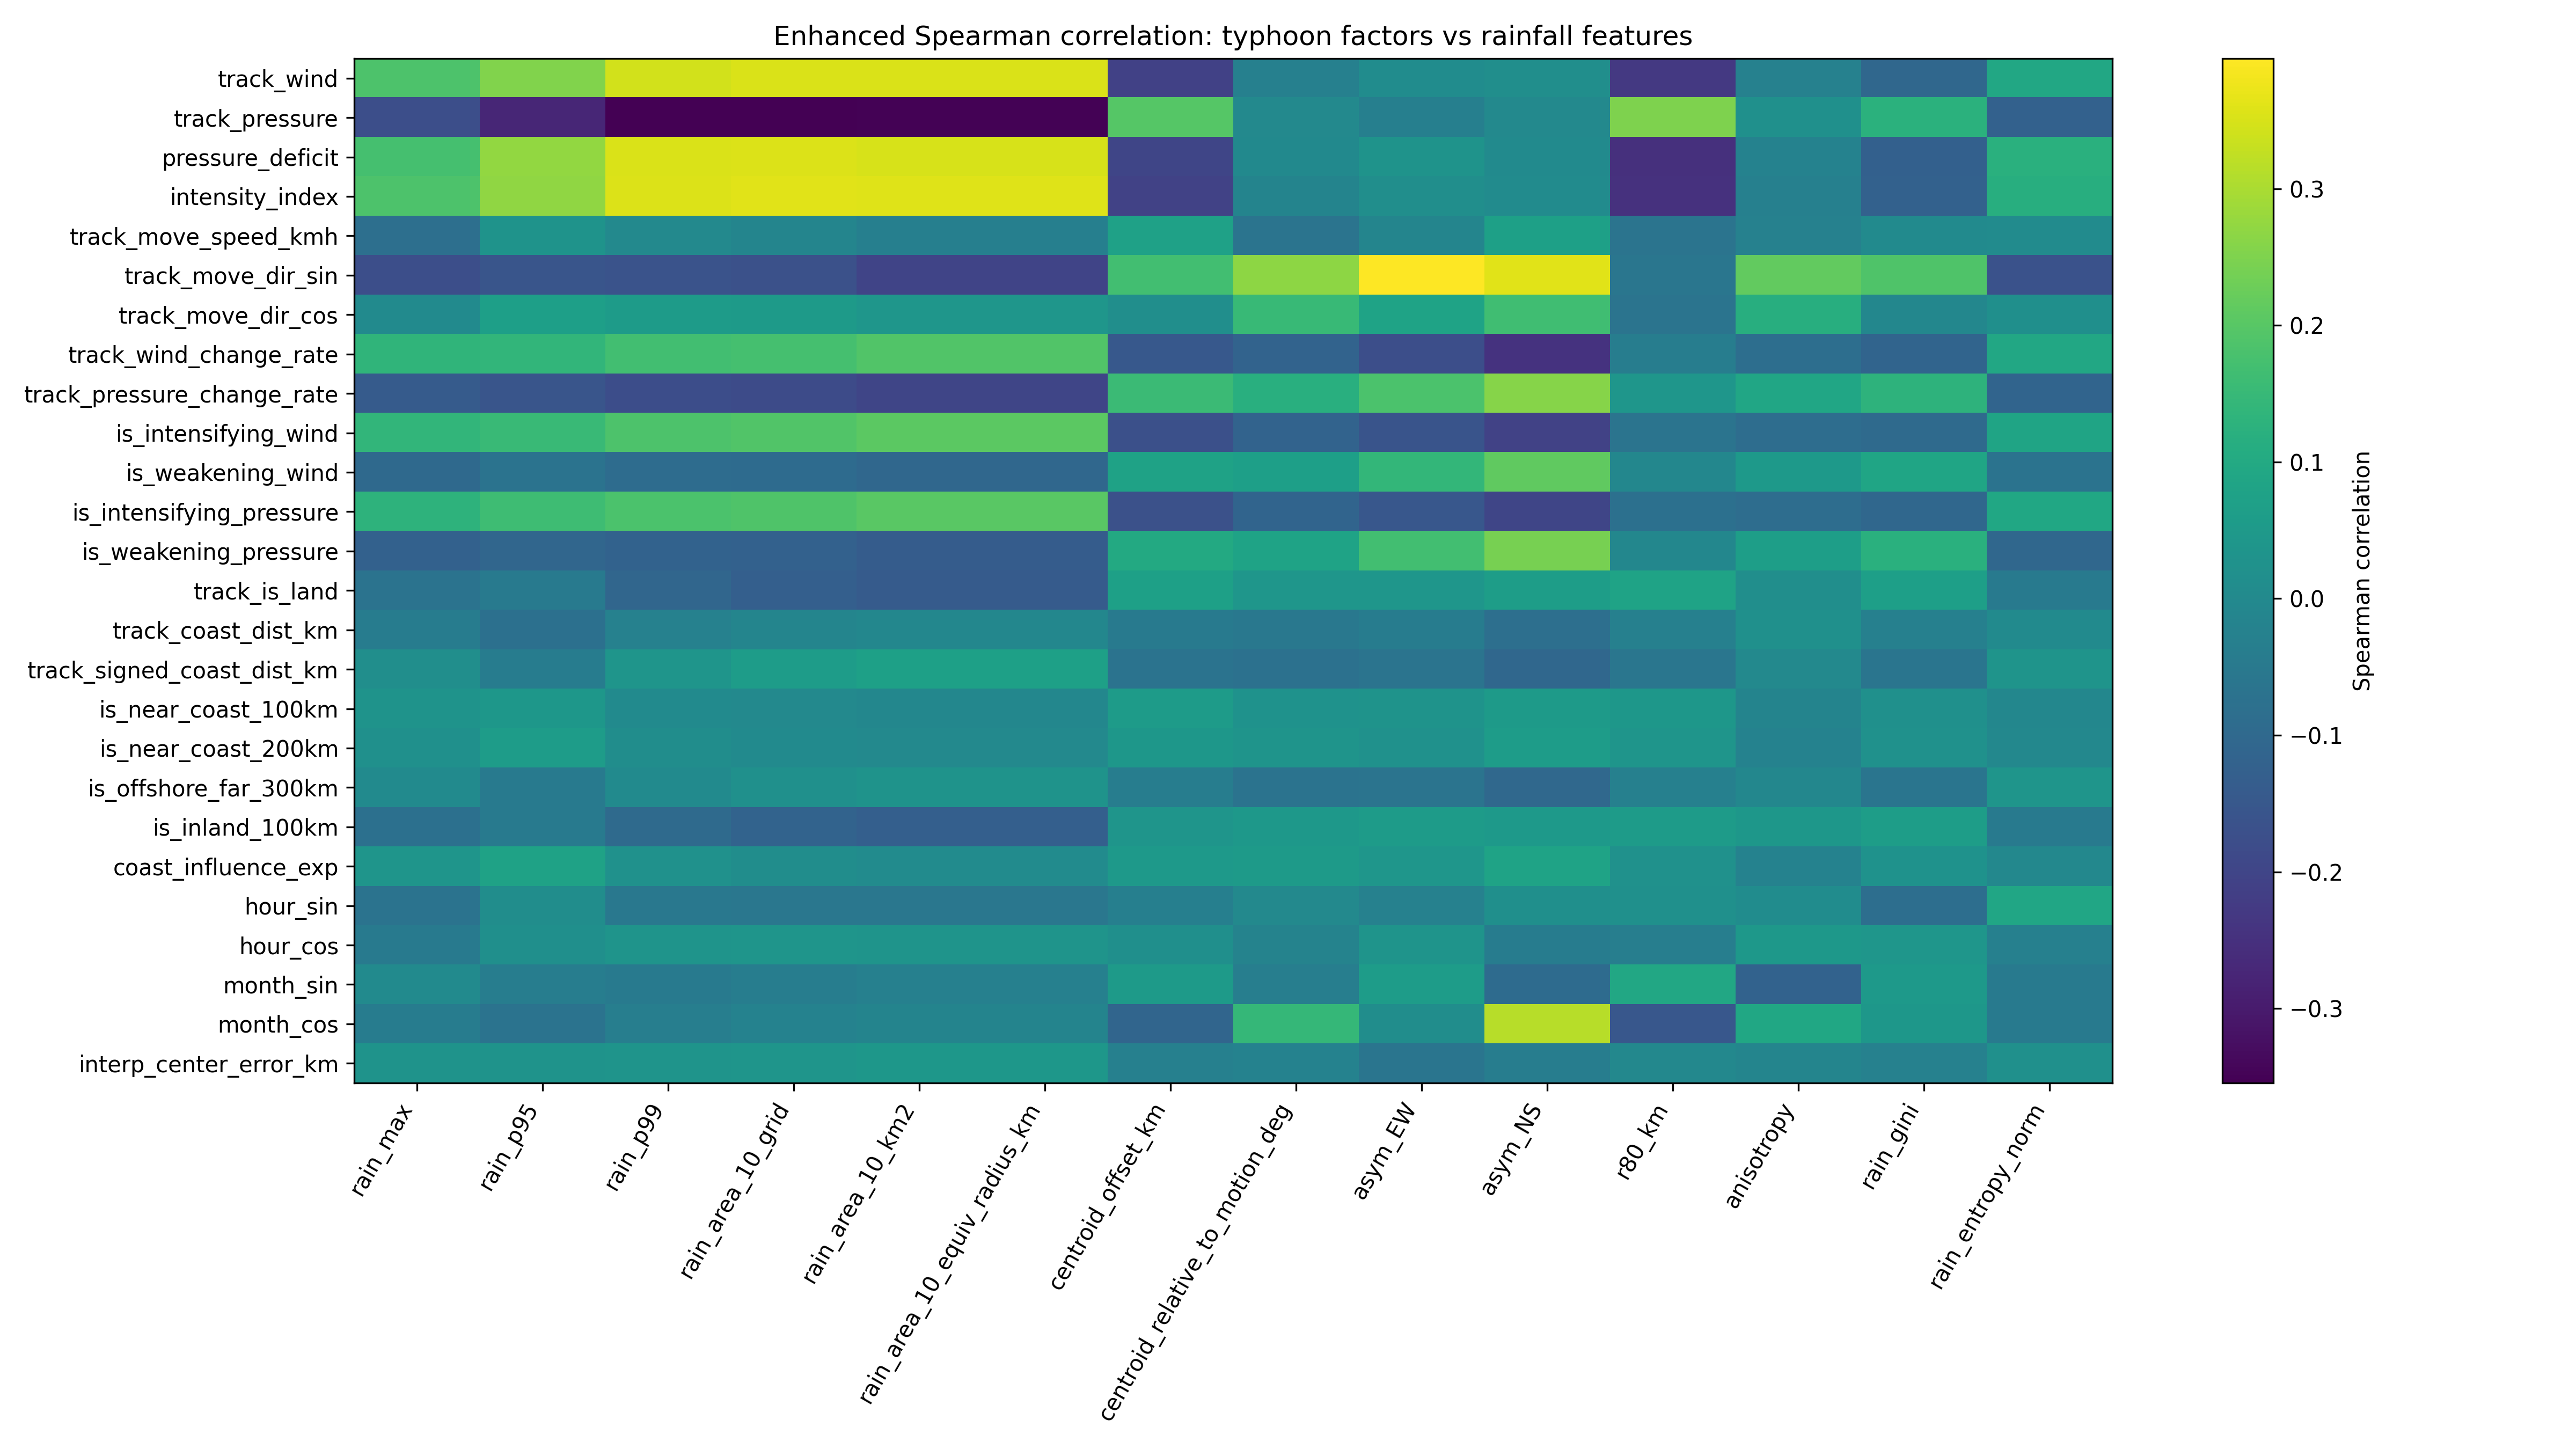
\includegraphics[width=0.95\textwidth]{01_enhanced_spearman_heatmap.png}
    \caption{路径、强度、环境因子与降水分布特征的Spearman相关性热力图}
    \label{fig:spearman_heatmap_problem1}
\end{figure}

\subsubsection{增强随机森林解释模型}

由于台风降水分布受多因素共同影响，且变量之间可能存在非线性关系，本文进一步建立增强随机森林回归模型。对每一个降水响应变量$Y_k$，以路径、强度、海陆和时间背景变量组成特征向量$\mathbf{X}_t$，建立模型：
\begin{equation}
    Y_{k,t}=f_k(\mathbf{X}_t)+\varepsilon_t.
\end{equation}
其中$f_k(\cdot)$由随机森林模型拟合，$\varepsilon_t$为残差项。本文使用的随机森林主要参数为：树数量$n_{\mathrm{estimators}}=250$，最大深度$max\_depth=14$，叶节点最小样本数$min\_samples\_leaf=20$。训练集和测试集按$3:1$随机划分，并采用置换重要性衡量不同解释变量对目标变量的贡献。

随机森林置换重要性定义为：在测试集上随机打乱某一特征后，模型预测性能下降的幅度。若某变量被打乱后模型性能下降越大，则说明该变量对解释目标降水特征越重要。

\subsection{模型求解结果}

\subsubsection{模型总体拟合效果}

基于插值后的半小时路径--降水联合样本，本文对六个主要降水响应变量分别建立增强随机森林模型。模型测试集$R^2$结果如表\ref{tab:rf_r2_problem1}所示。

\begin{table}[htbp]
    \centering
    \caption{增强随机森林模型对主要降水分布特征的解释效果}
    \label{tab:rf_r2_problem1}
    \begin{tabular}{lcc}
        \hline
        响应变量 & 含义 & 测试集$R^2$ \\
        \hline
        $rain\_max$ & 单点最大降水强度 & 0.406 \\
        $rain\_p95$ & P95降水强度 & 0.648 \\
        $rain\_area\_10\_km^2$ & 强降水面积 & 0.584 \\
        $rain\_area\_10\_equiv\_radius$ & 强降水等效半径 & 0.642 \\
        $centroid\_offset$ & 降水质心偏移 & 0.672 \\
        $anisotropy$ & 雨带各向异性 & 0.636 \\
        \hline
    \end{tabular}
\end{table}

由表\ref{tab:rf_r2_problem1}可见，模型对P95降水强度、强降水等效半径、降水质心偏移和雨带各向异性的测试集$R^2$均超过0.63，说明路径、强度、移动、海陆和季节背景特征能够较好解释台风降水空间结构的主要变化。相比之下，单点最大降水强度$rain\_max$的$R^2$为0.406，解释能力相对较弱。这主要是因为单点最大值更容易受到局地强对流、遥感反演误差和孤立极值格点影响，稳定性弱于分位数和面积类指标。

\subsubsection{台风强度对降水强度与强降水范围的影响}

Spearman相关性结果显示，P95降水强度与中心气压呈负相关，与气压亏损、综合强度指数和最大风速呈正相关。其中，$rain\_p95$与中心气压的相关系数为$-0.274$，与气压亏损的相关系数为$0.274$，与综合强度指数的相关系数为$0.271$，与最大风速的相关系数为$0.254$。

对于强降水面积$rain\_area\_10\_km^2$，其与综合强度指数的相关系数为$0.358$，与最大风速的相关系数为$0.352$，与中心气压的相关系数为$-0.350$，与气压亏损的相关系数为$0.350$。这表明台风强度是降水强度和强降水范围的主控因子。中心气压越低、气压亏损越大、最大风速越高，台风的强降水水平和强降水覆盖范围越大。

图\ref{fig:intensity_p95_problem1}和图\ref{fig:intensity_area10_problem1}分别展示了综合强度指数与P95降水强度、强降水面积之间的关系。

\begin{figure}[htbp]
    \centering
    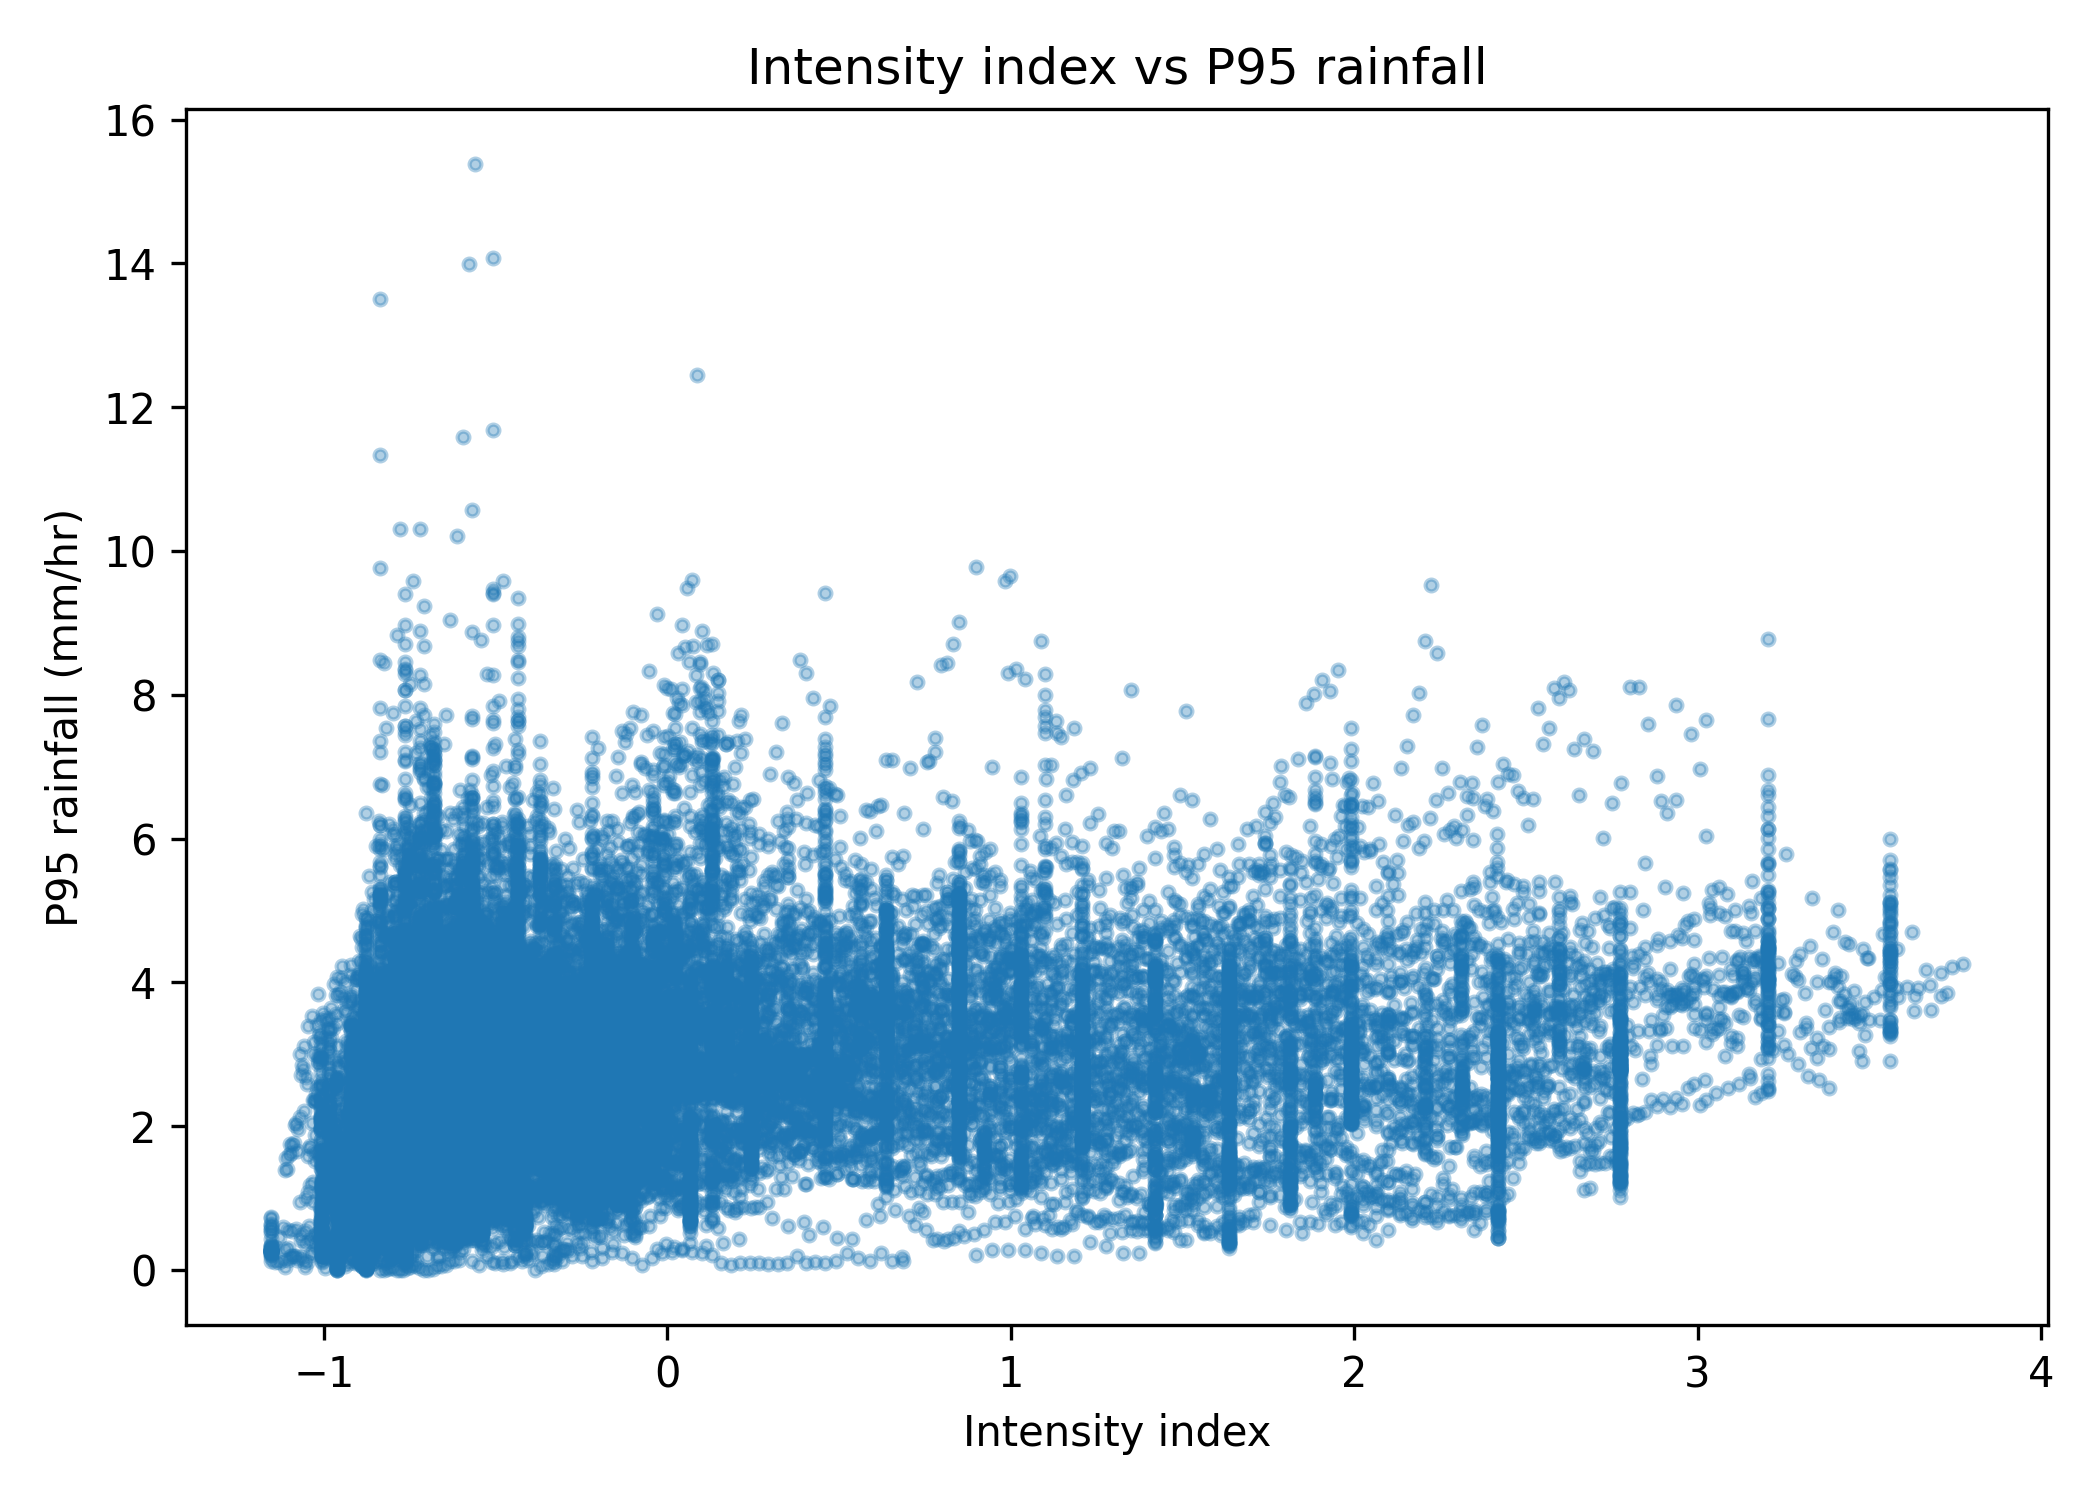
\includegraphics[width=0.72\textwidth]{02_intensity_index_vs_rain_p95.png}
    \caption{综合强度指数与P95降水强度的关系}
    \label{fig:intensity_p95_problem1}
\end{figure}

\begin{figure}[htbp]
    \centering
    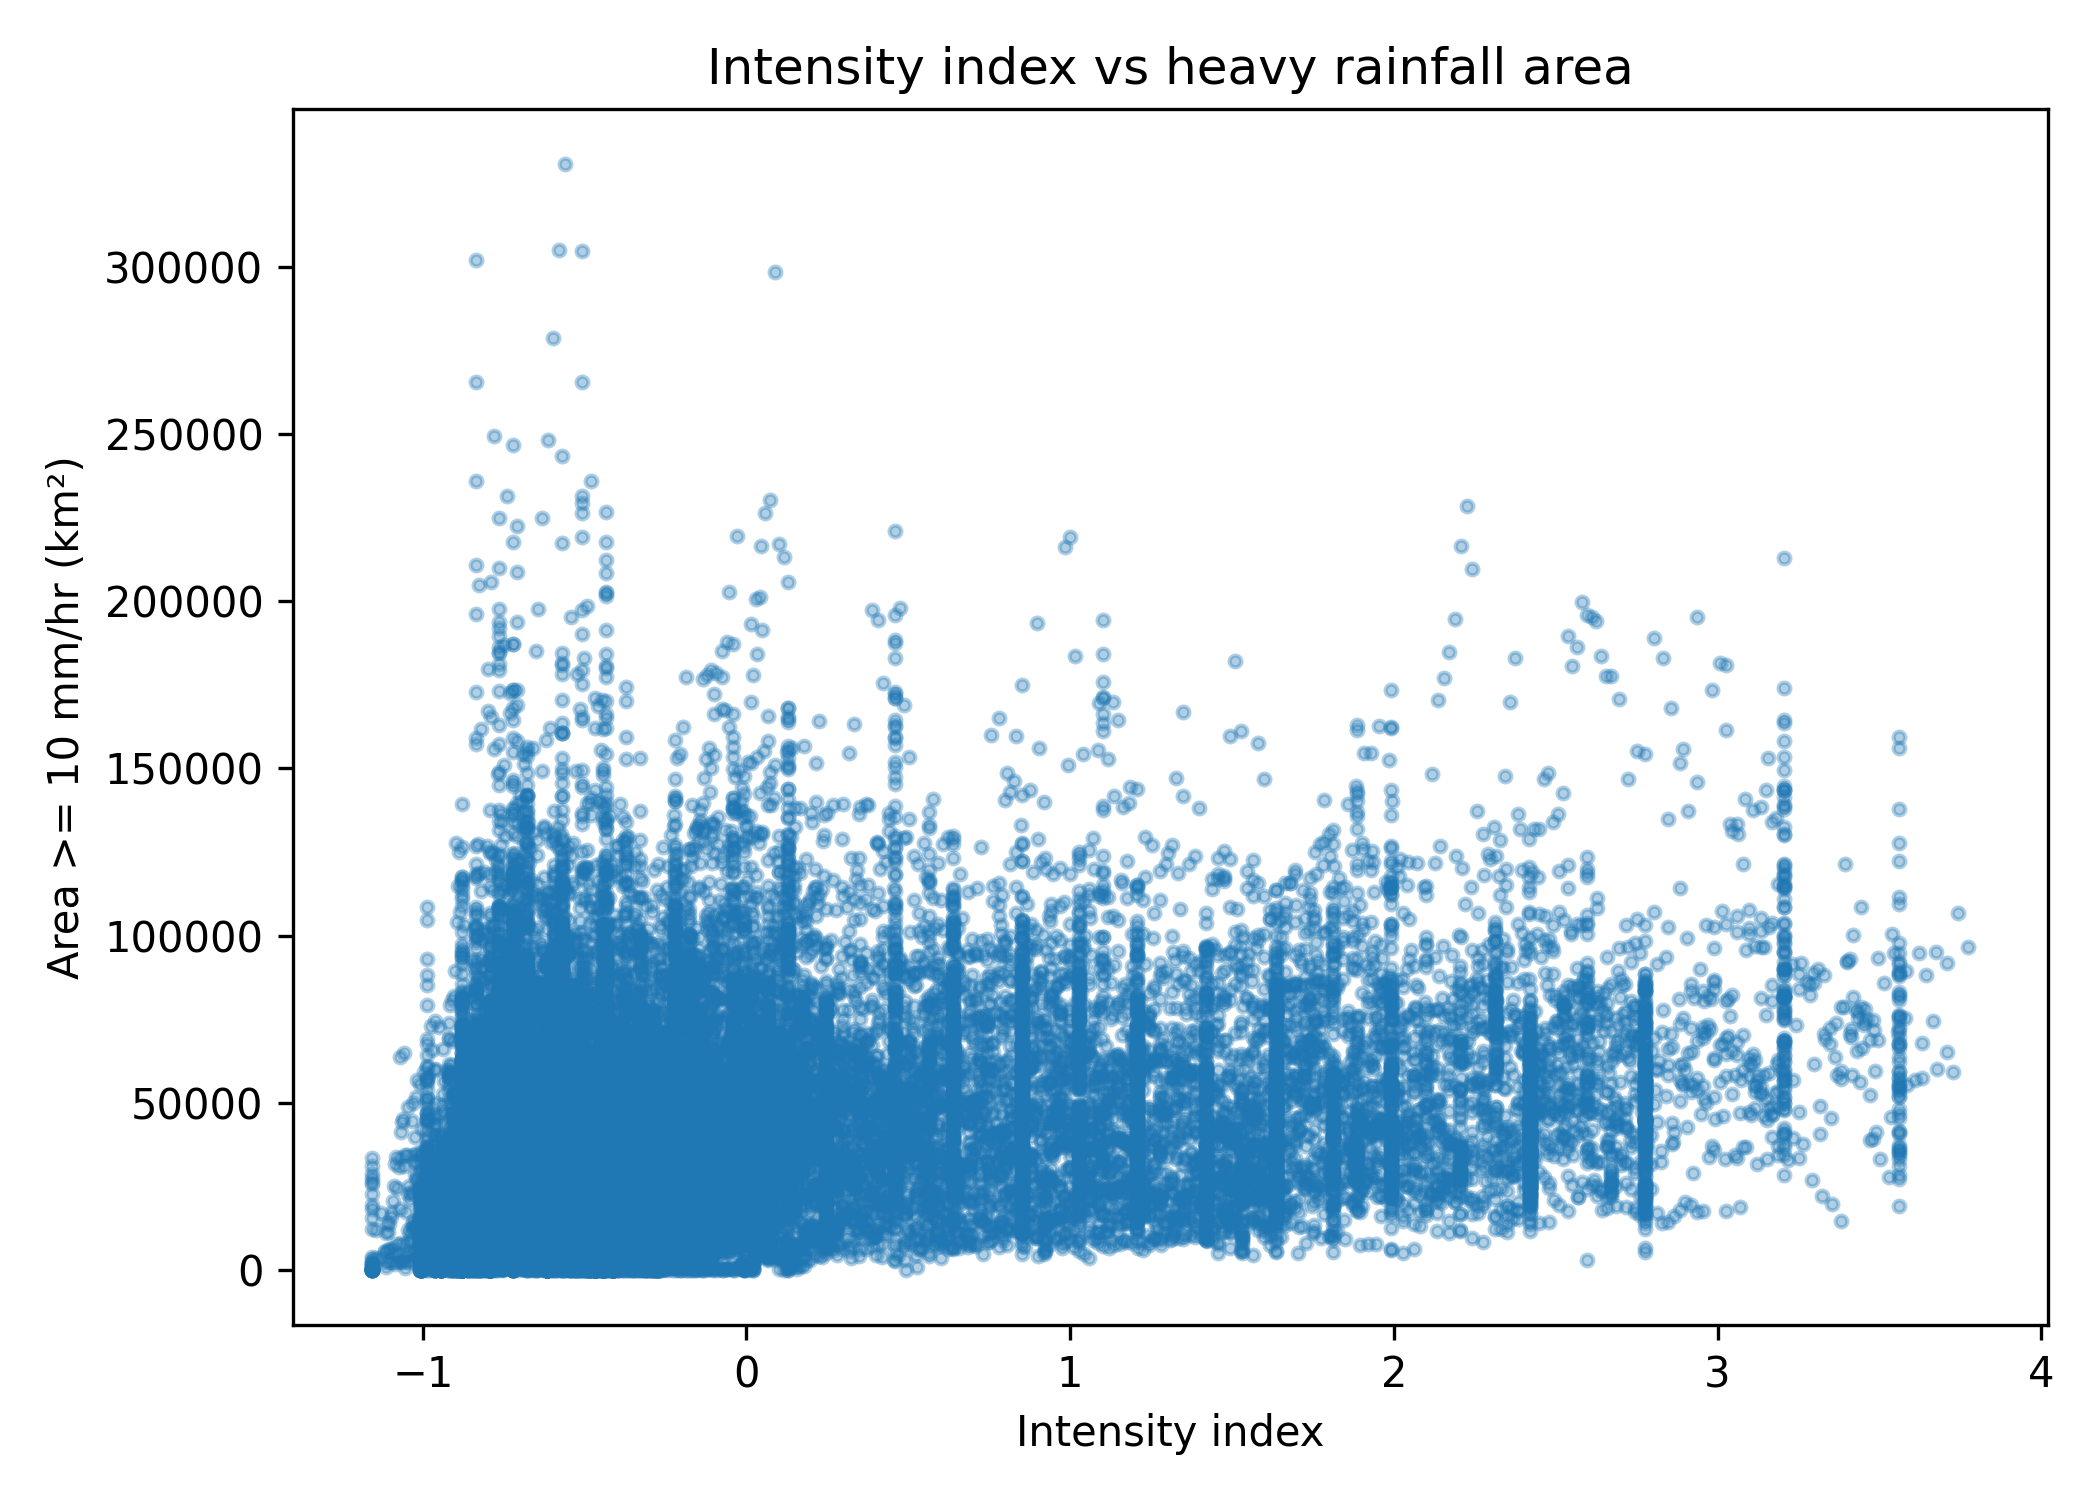
\includegraphics[width=0.72\textwidth]{03_intensity_index_vs_area10_km2.png}
    \caption{综合强度指数与强降水面积的关系}
    \label{fig:intensity_area10_problem1}
\end{figure}

随机森林置换重要性进一步支持上述结论。对于$rain\_p95$，移动方向正弦、月份余弦、综合强度指数、移动方向余弦和移动速度为前五个重要因素；对于$rain\_area\_10\_km^2$，移动方向正弦、最大风速、月份余弦、气压亏损和移动方向余弦为前五个重要因素。虽然随机森林中的变量重要性体现了非线性和交互效应，但强度相关变量始终位于前列，说明台风强度对降水强度和强降水范围具有稳定影响。

\begin{figure}[htbp]
    \centering
    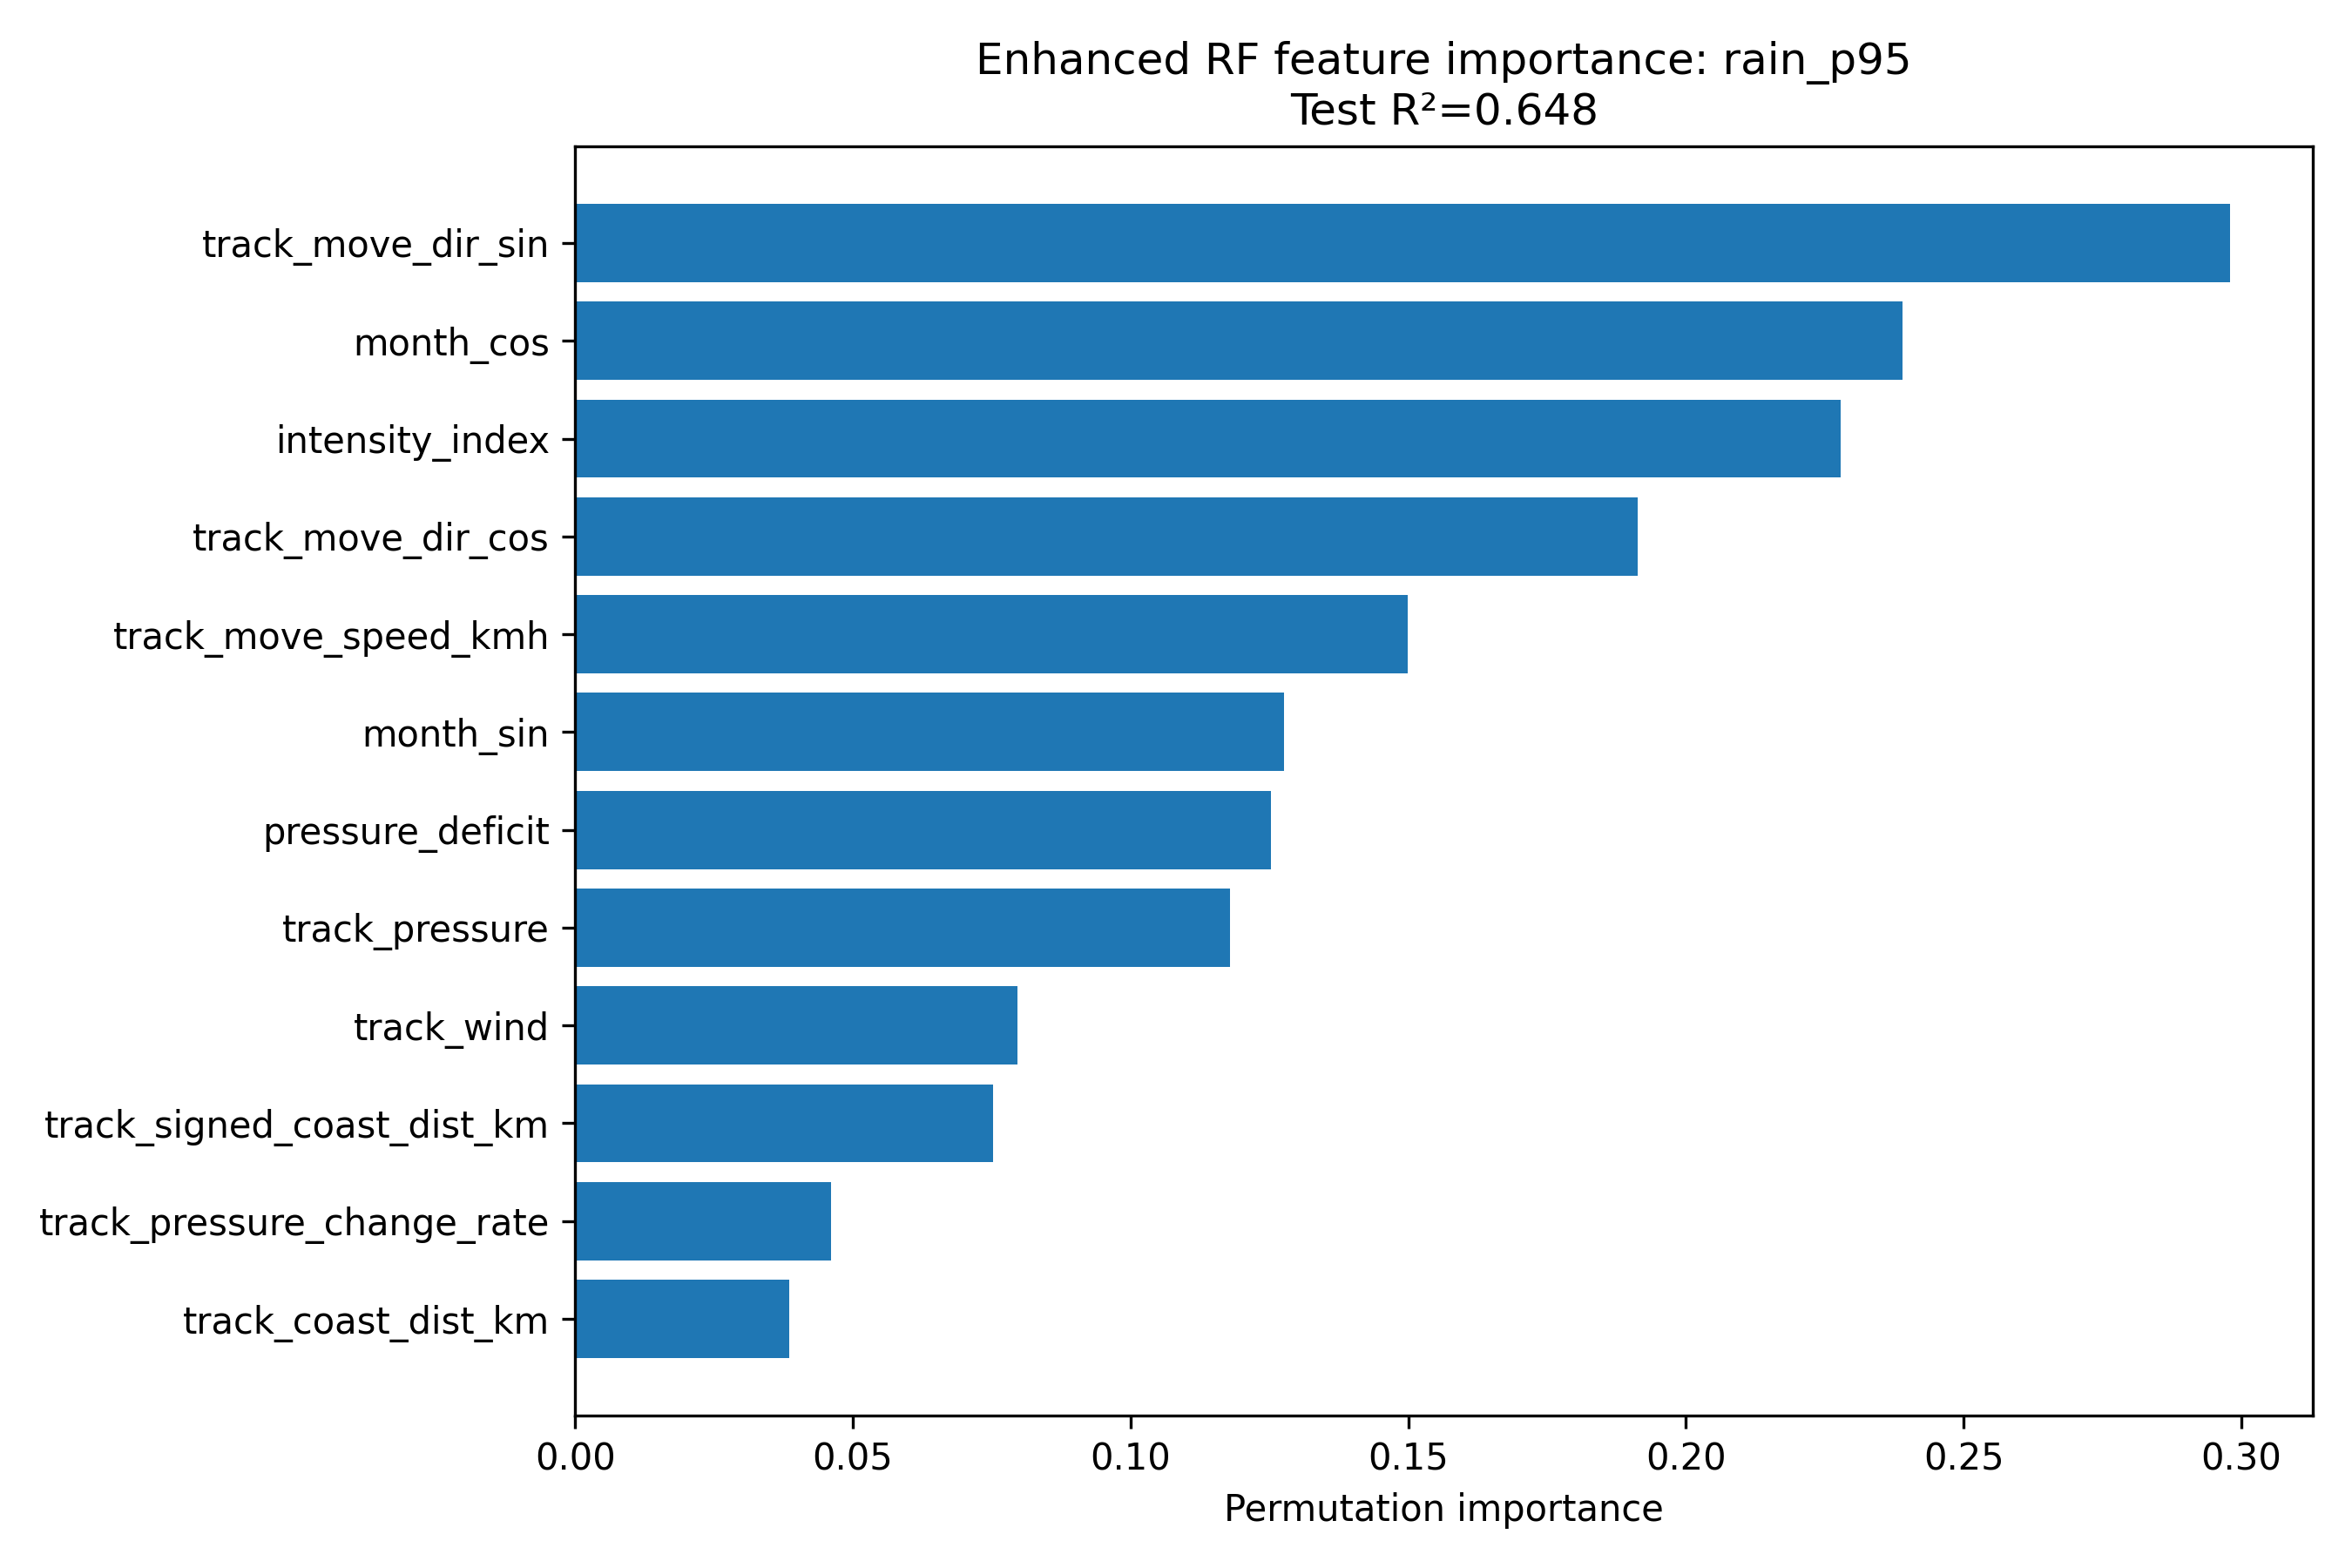
\includegraphics[width=0.78\textwidth]{07_enhanced_rf_importance_rain_p95.png}
    \caption{P95降水强度模型的随机森林特征重要性}
    \label{fig:rf_importance_p95_problem1}
\end{figure}

\begin{figure}[htbp]
    \centering
    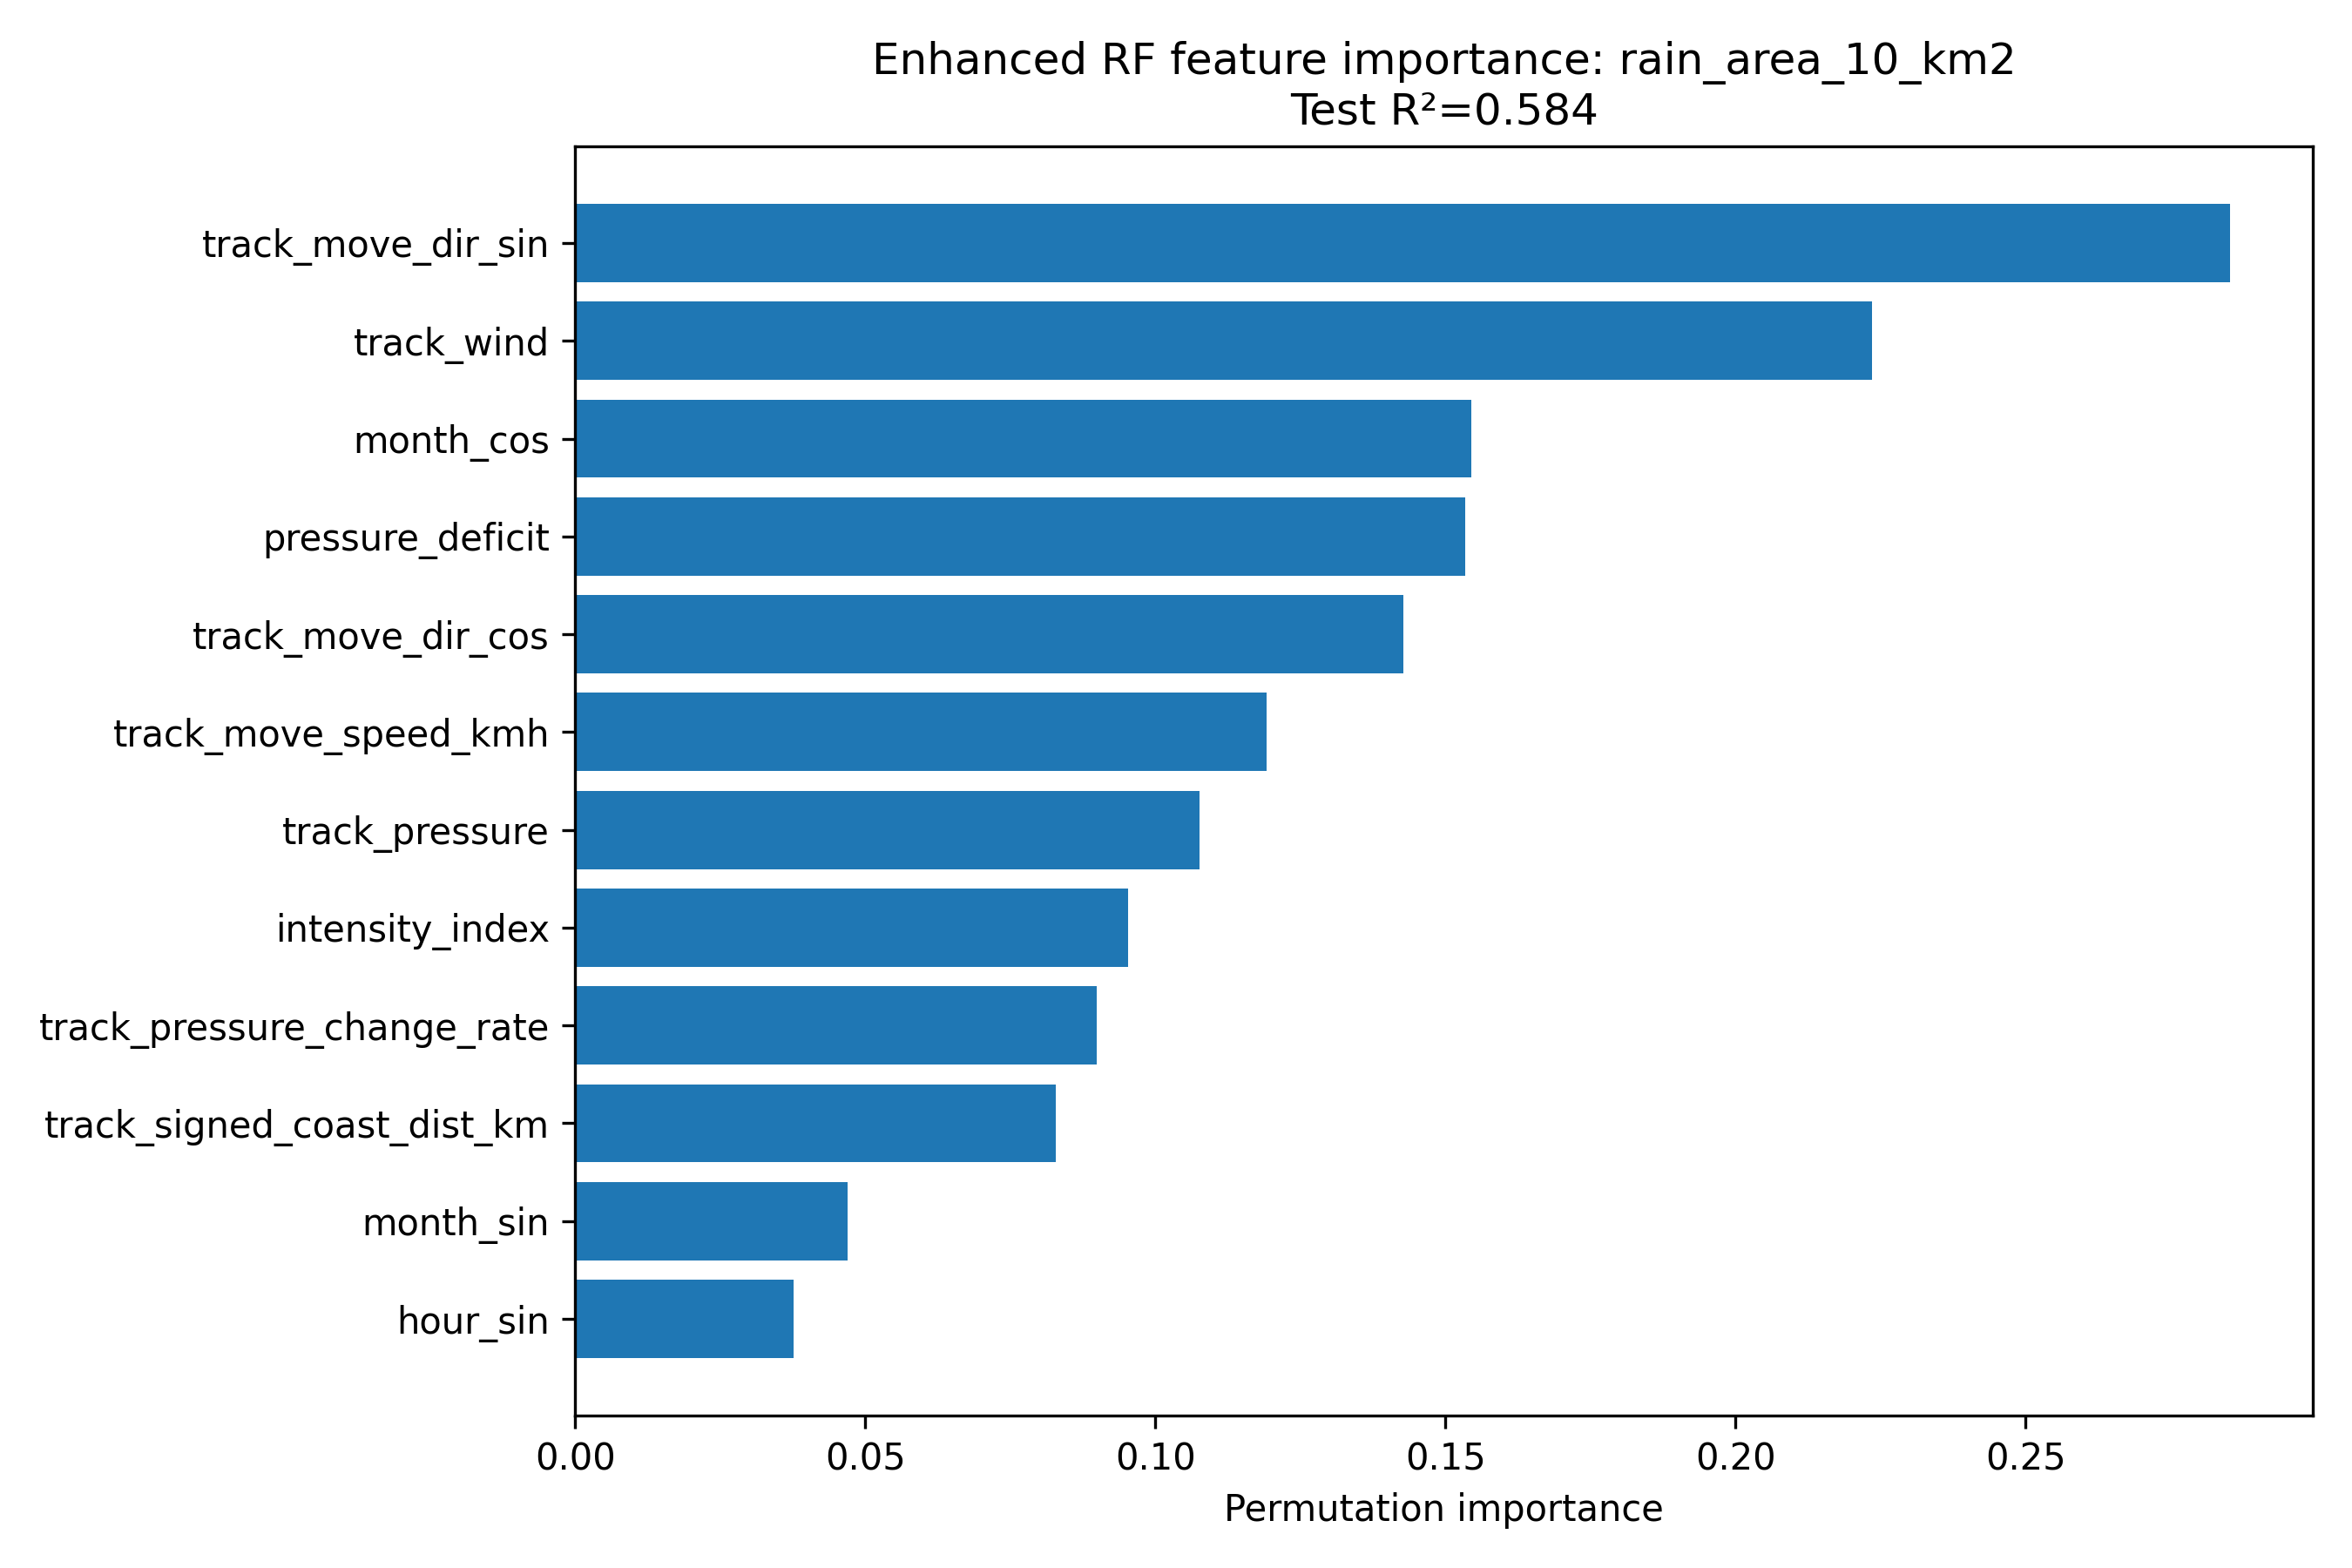
\includegraphics[width=0.78\textwidth]{07_enhanced_rf_importance_rain_area_10_km2.png}
    \caption{强降水面积模型的随机森林特征重要性}
    \label{fig:rf_importance_area10_problem1}
\end{figure}

\subsubsection{移动方向和移动速度对降水空间结构的影响}

降水质心偏移模型的测试集$R^2$为0.672，是本问题中解释效果较好的目标变量之一。随机森林结果显示，影响降水质心偏移的前五个变量依次为：移动方向正弦、移动速度、月份余弦、综合强度指数和移动方向余弦。说明降水中心相对于台风中心的偏移不仅与台风强度有关，也显著受到台风移动方向和移动速度影响。

图\ref{fig:move_centroid_problem1}展示了移动速度与降水质心偏移之间的关系。总体来看，移动速度越大，降水质心偏移的变化范围越大，说明台风移动过程会改变水汽输送和降水落区相对于台风中心的位置。

\begin{figure}[htbp]
    \centering
    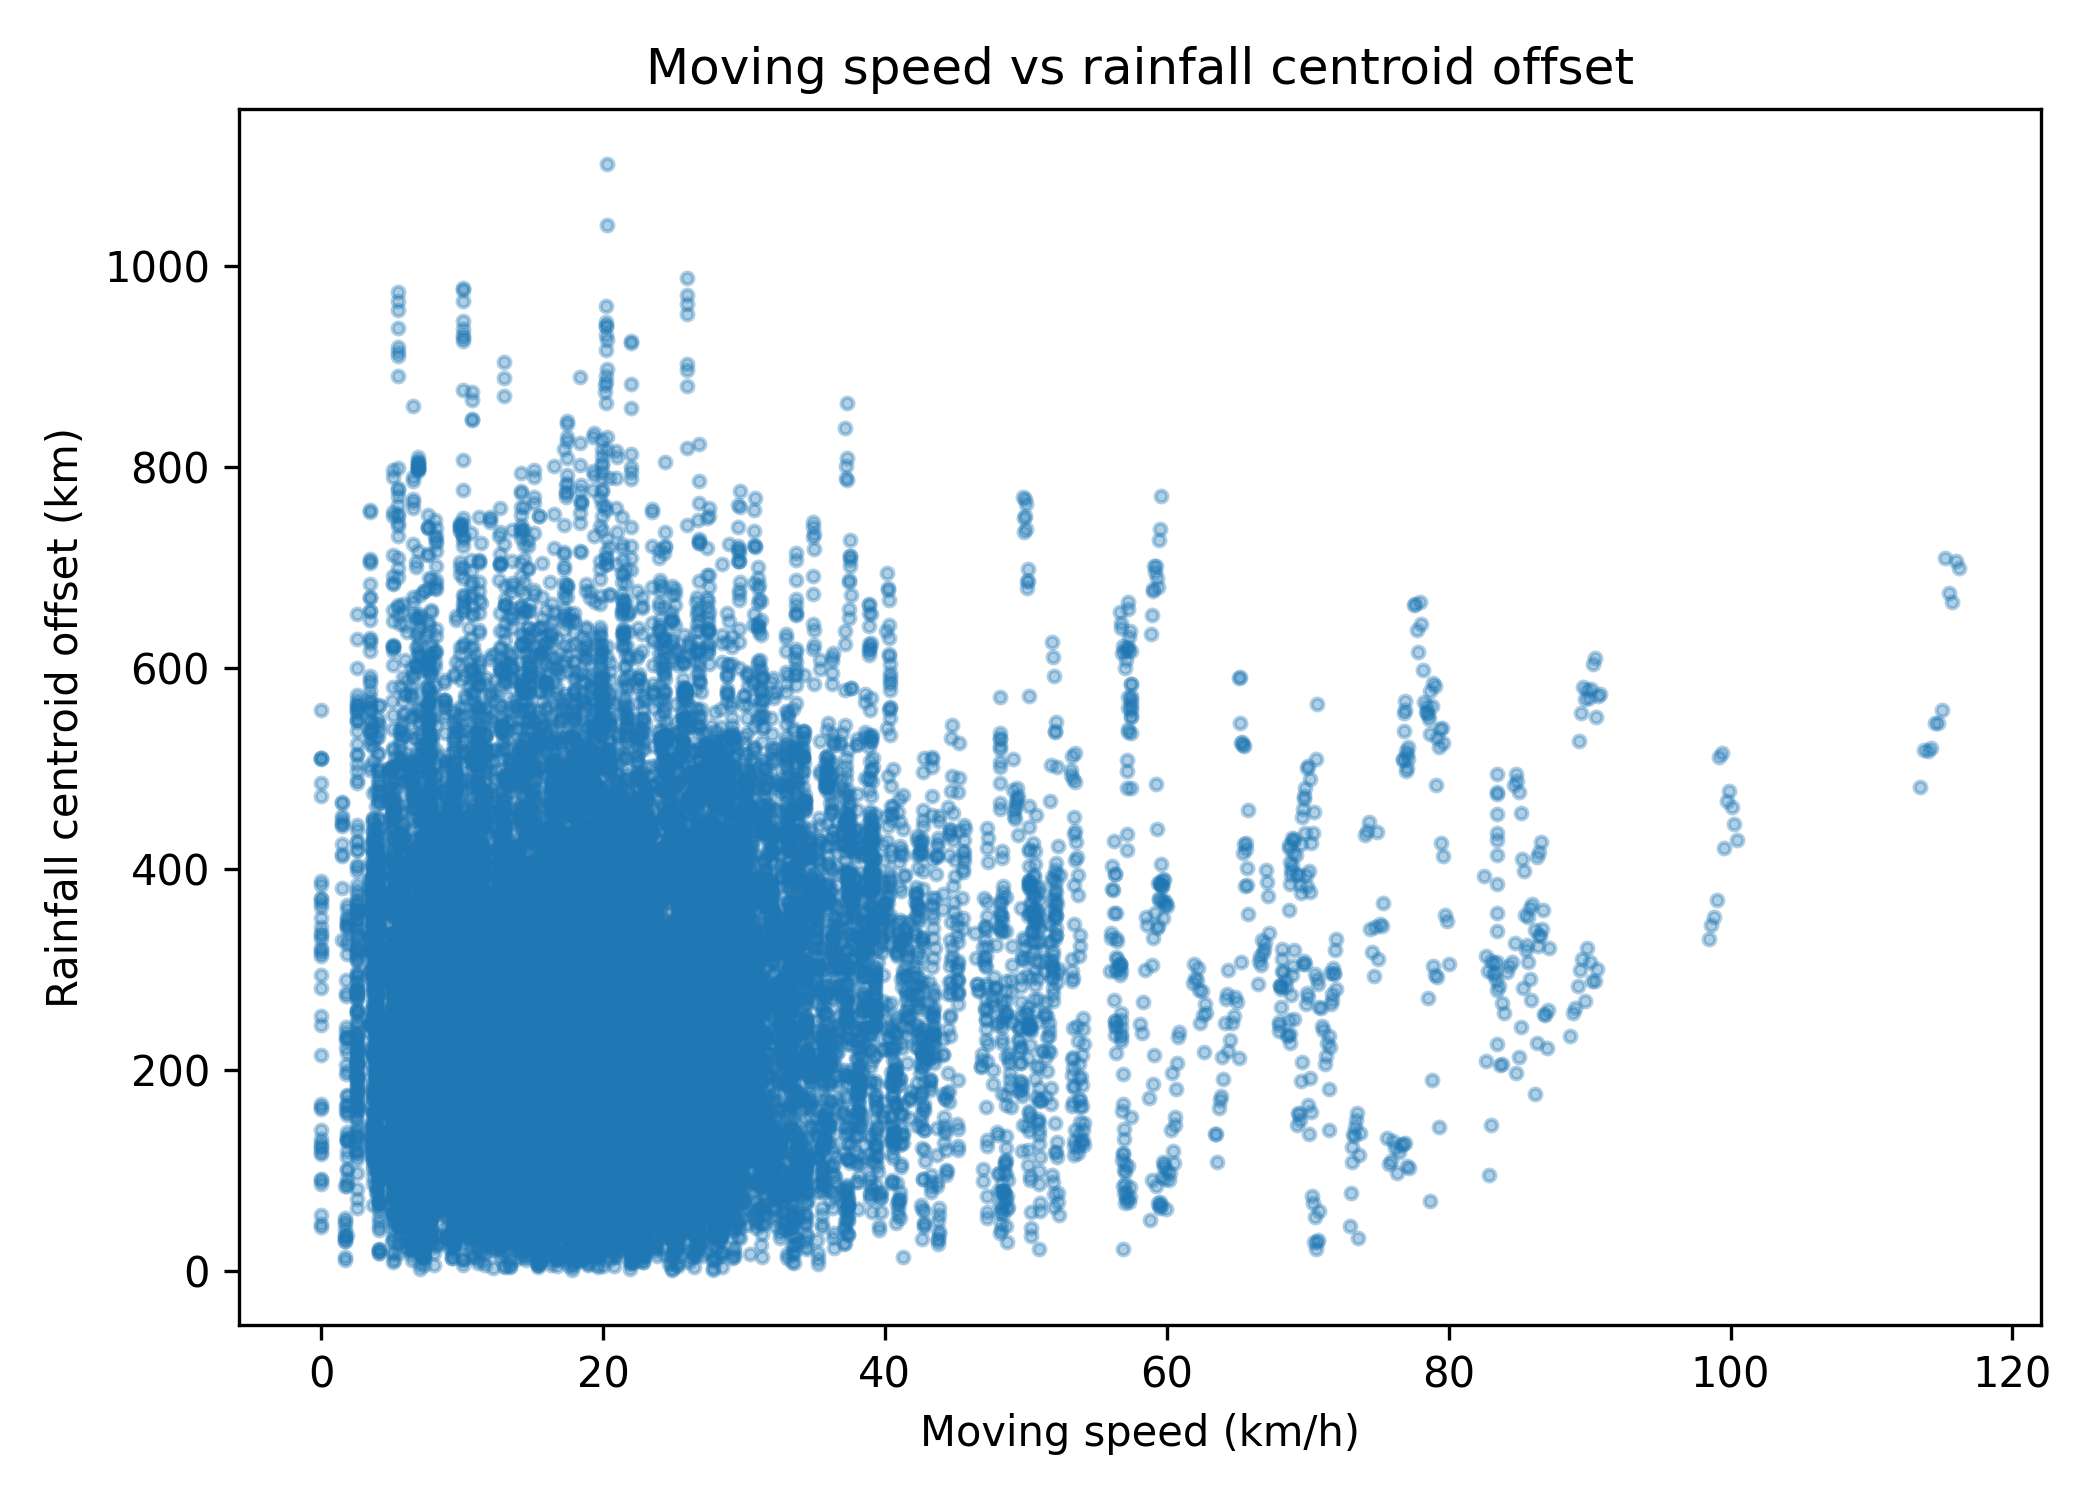
\includegraphics[width=0.72\textwidth]{05_move_speed_vs_centroid_offset.png}
    \caption{移动速度与降水质心偏移的关系}
    \label{fig:move_centroid_problem1}
\end{figure}

雨带各向异性模型的测试集$R^2$为0.636。其前五个重要变量依次为：移动方向正弦、移动速度、月份余弦、移动方向余弦和月份正弦。这说明雨带是否呈狭长形态与台风行进方向和移动速度密切相关。移动方向正弦和余弦同时进入前列，也表明用周期变量表示移动方向是必要的。

\begin{figure}[htbp]
    \centering
    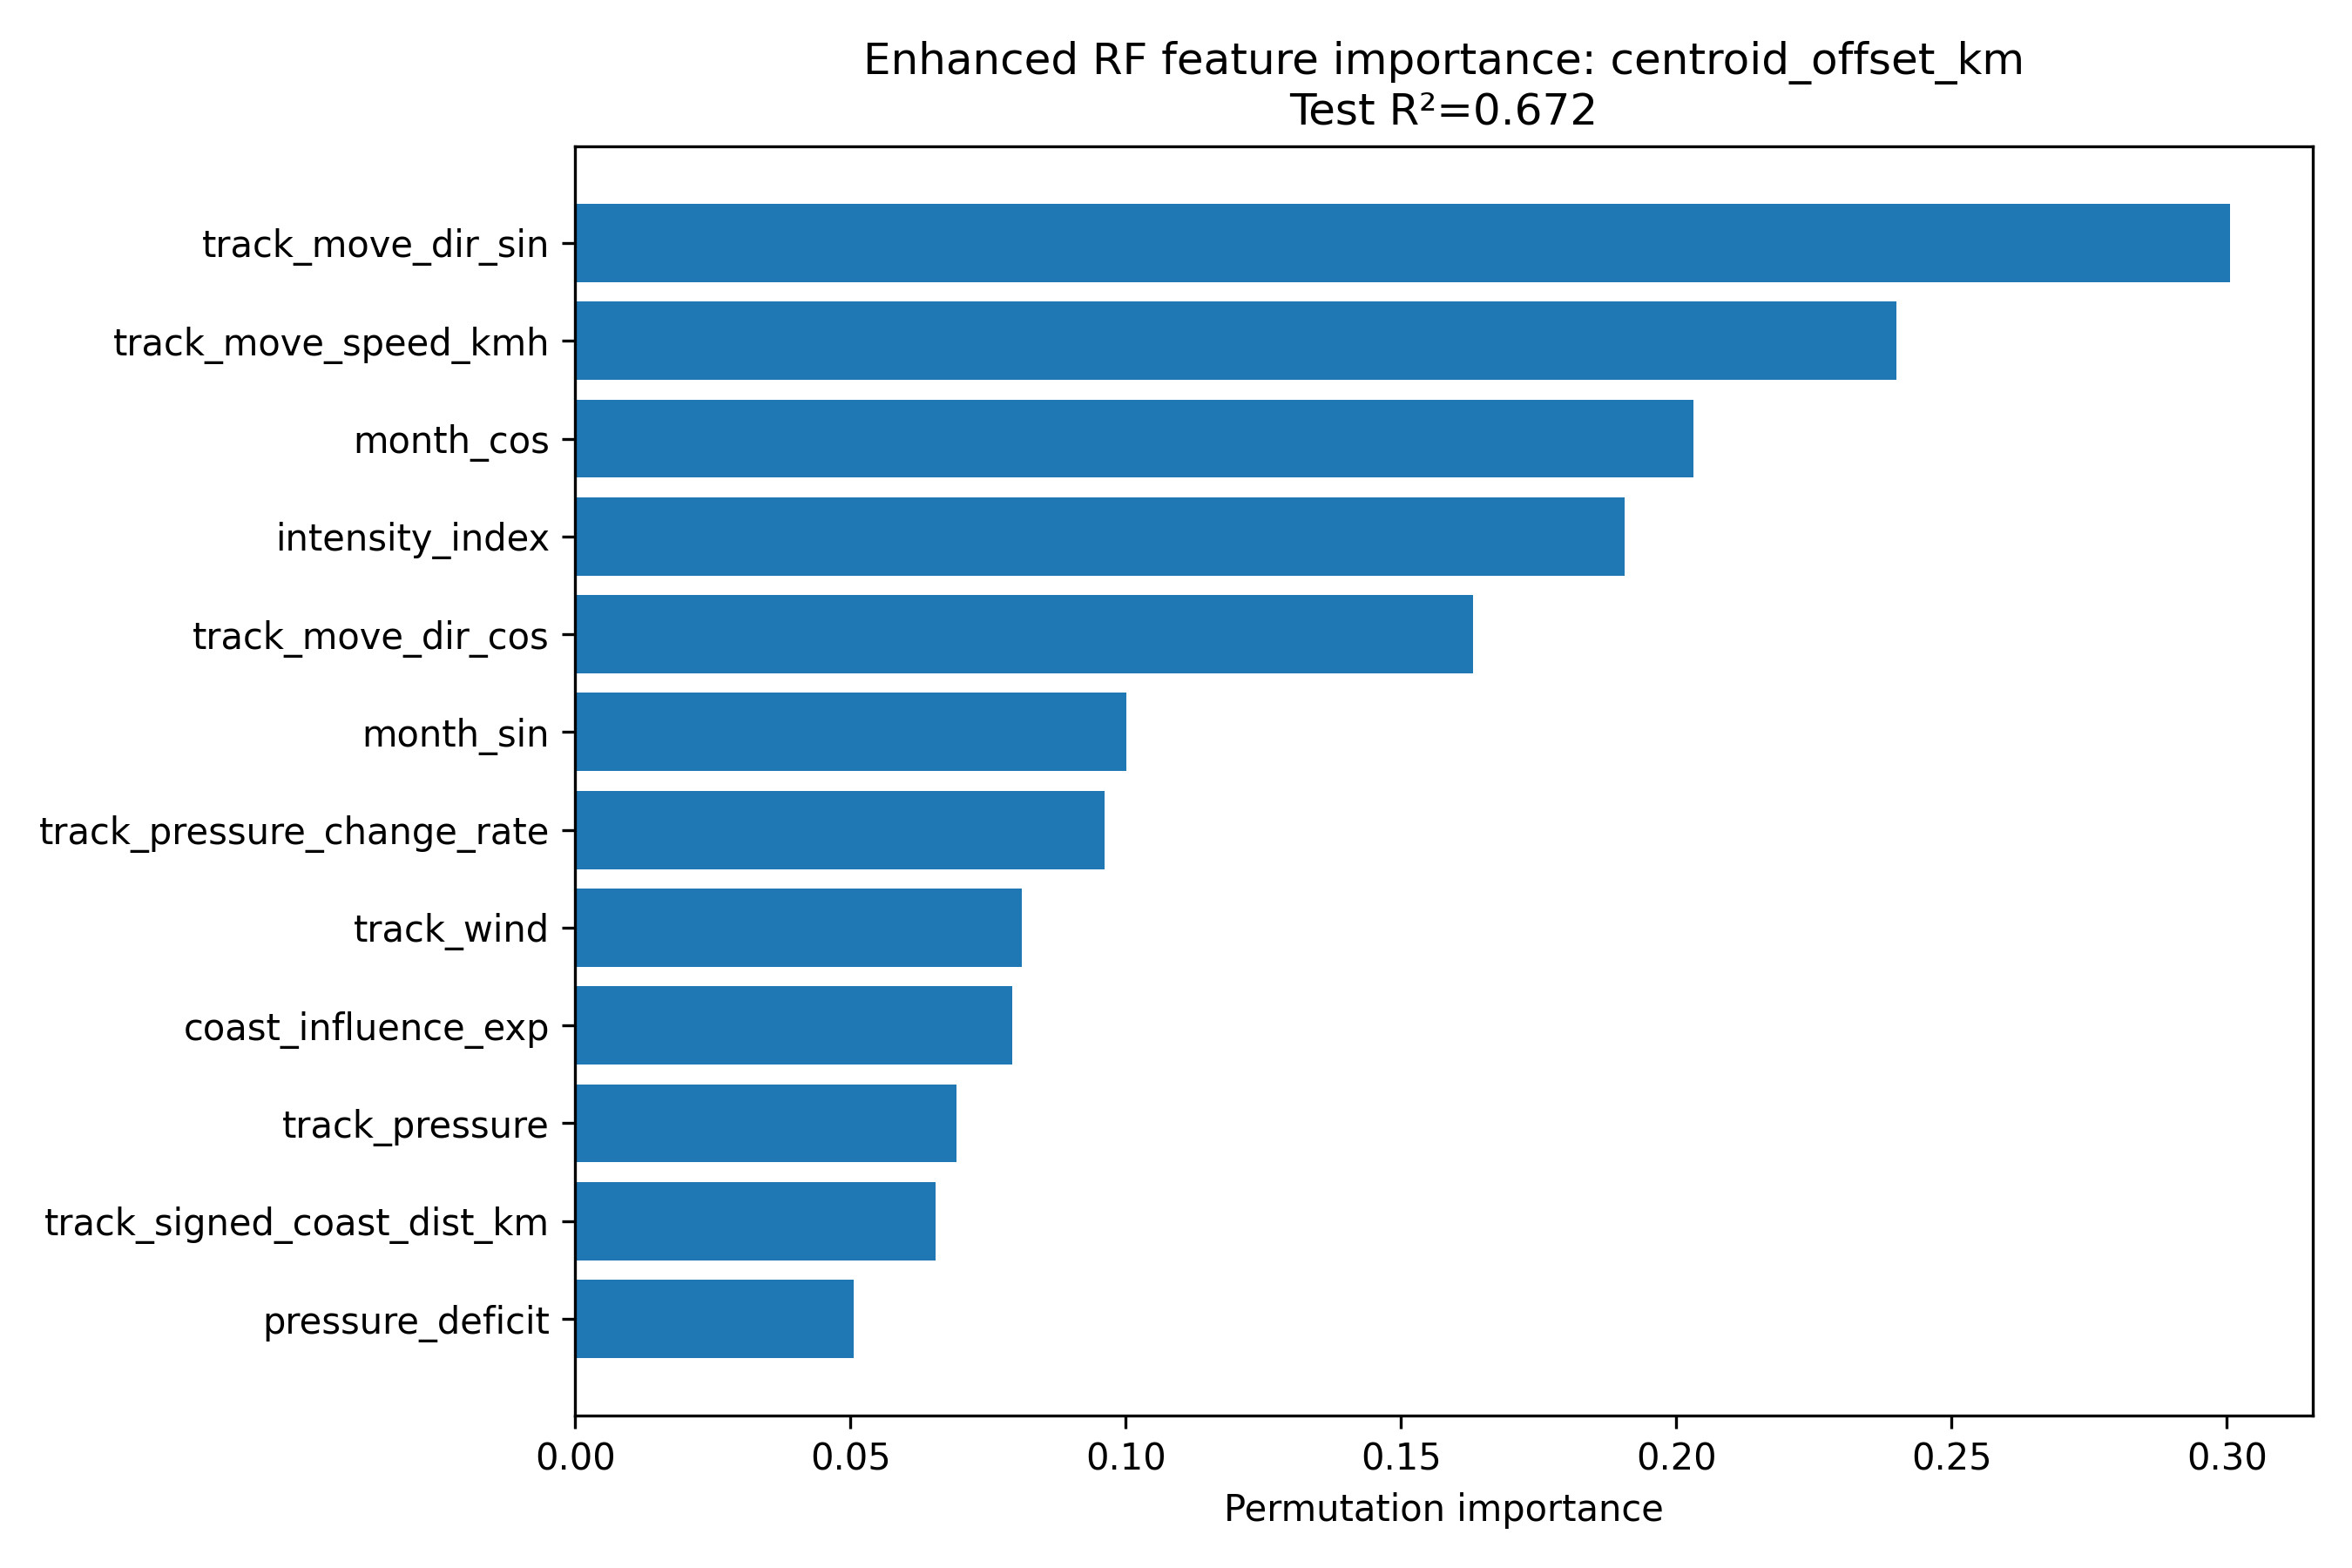
\includegraphics[width=0.78\textwidth]{07_enhanced_rf_importance_centroid_offset_km.png}
    \caption{降水质心偏移模型的随机森林特征重要性}
    \label{fig:rf_importance_centroid_problem1}
\end{figure}

\begin{figure}[htbp]
    \centering
    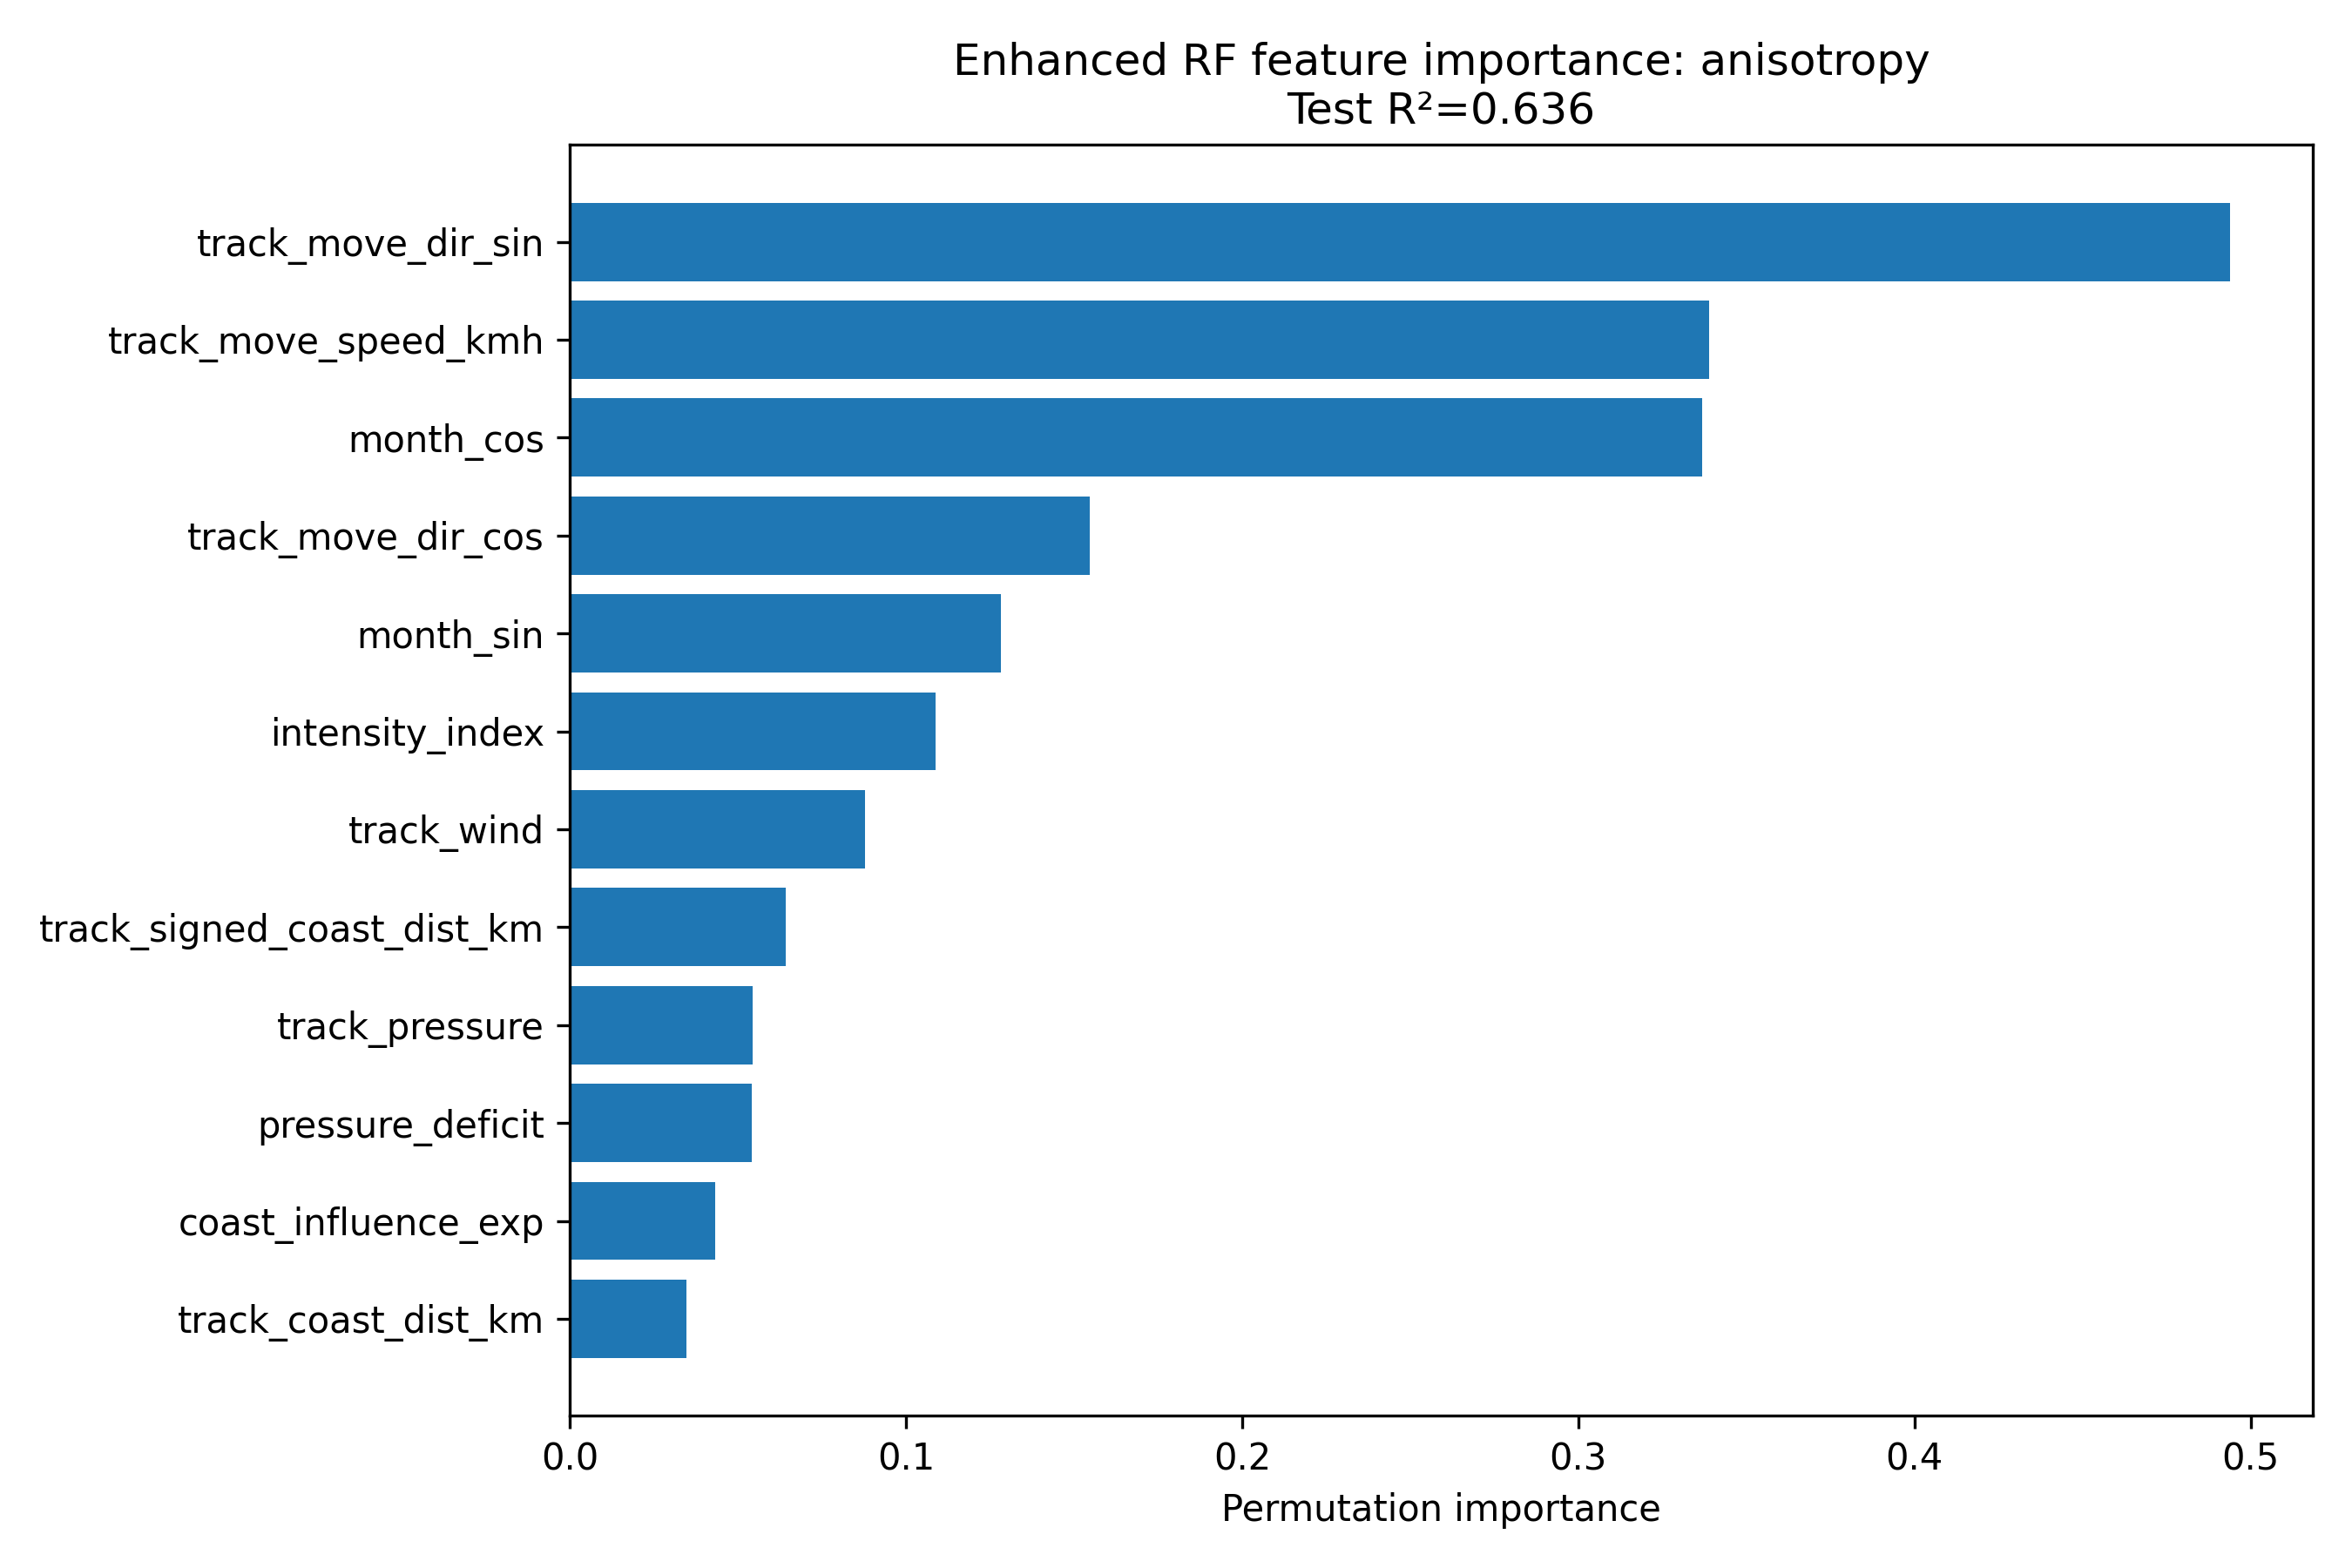
\includegraphics[width=0.78\textwidth]{07_enhanced_rf_importance_anisotropy.png}
    \caption{雨带各向异性模型的随机森林特征重要性}
    \label{fig:rf_importance_anisotropy_problem1}
\end{figure}

\subsubsection{固定地理方向下降水非对称性与台风演变的关系}

相关性结果显示，东西方向非对称性$asym\_EW$与移动方向正弦的Spearman相关系数为$0.395$，与气压变化率的相关系数为$0.184$，与风速变化率的相关系数为$-0.174$。南北方向非对称性$asym\_NS$与移动方向正弦的相关系数为$0.362$，与月份余弦的相关系数为$0.315$，与气压变化率的相关系数为$0.258$，与风速变化率的相关系数为$-0.245$。

这些结果表明，固定地理方向下的降水非对称性不是单纯由当前风速或中心气压决定，而与台风移动方向、增强或减弱过程以及季节背景共同相关。换言之，台风降水空间偏向不仅反映台风当前强度，也反映台风演变状态和背景环流条件。

图\ref{fig:centroid_motion_hist_problem1}展示了降水质心方向相对于台风移动方向的分布，用于辅助说明降水偏移与台风运动方向之间的联系。

\begin{figure}[htbp]
    \centering
    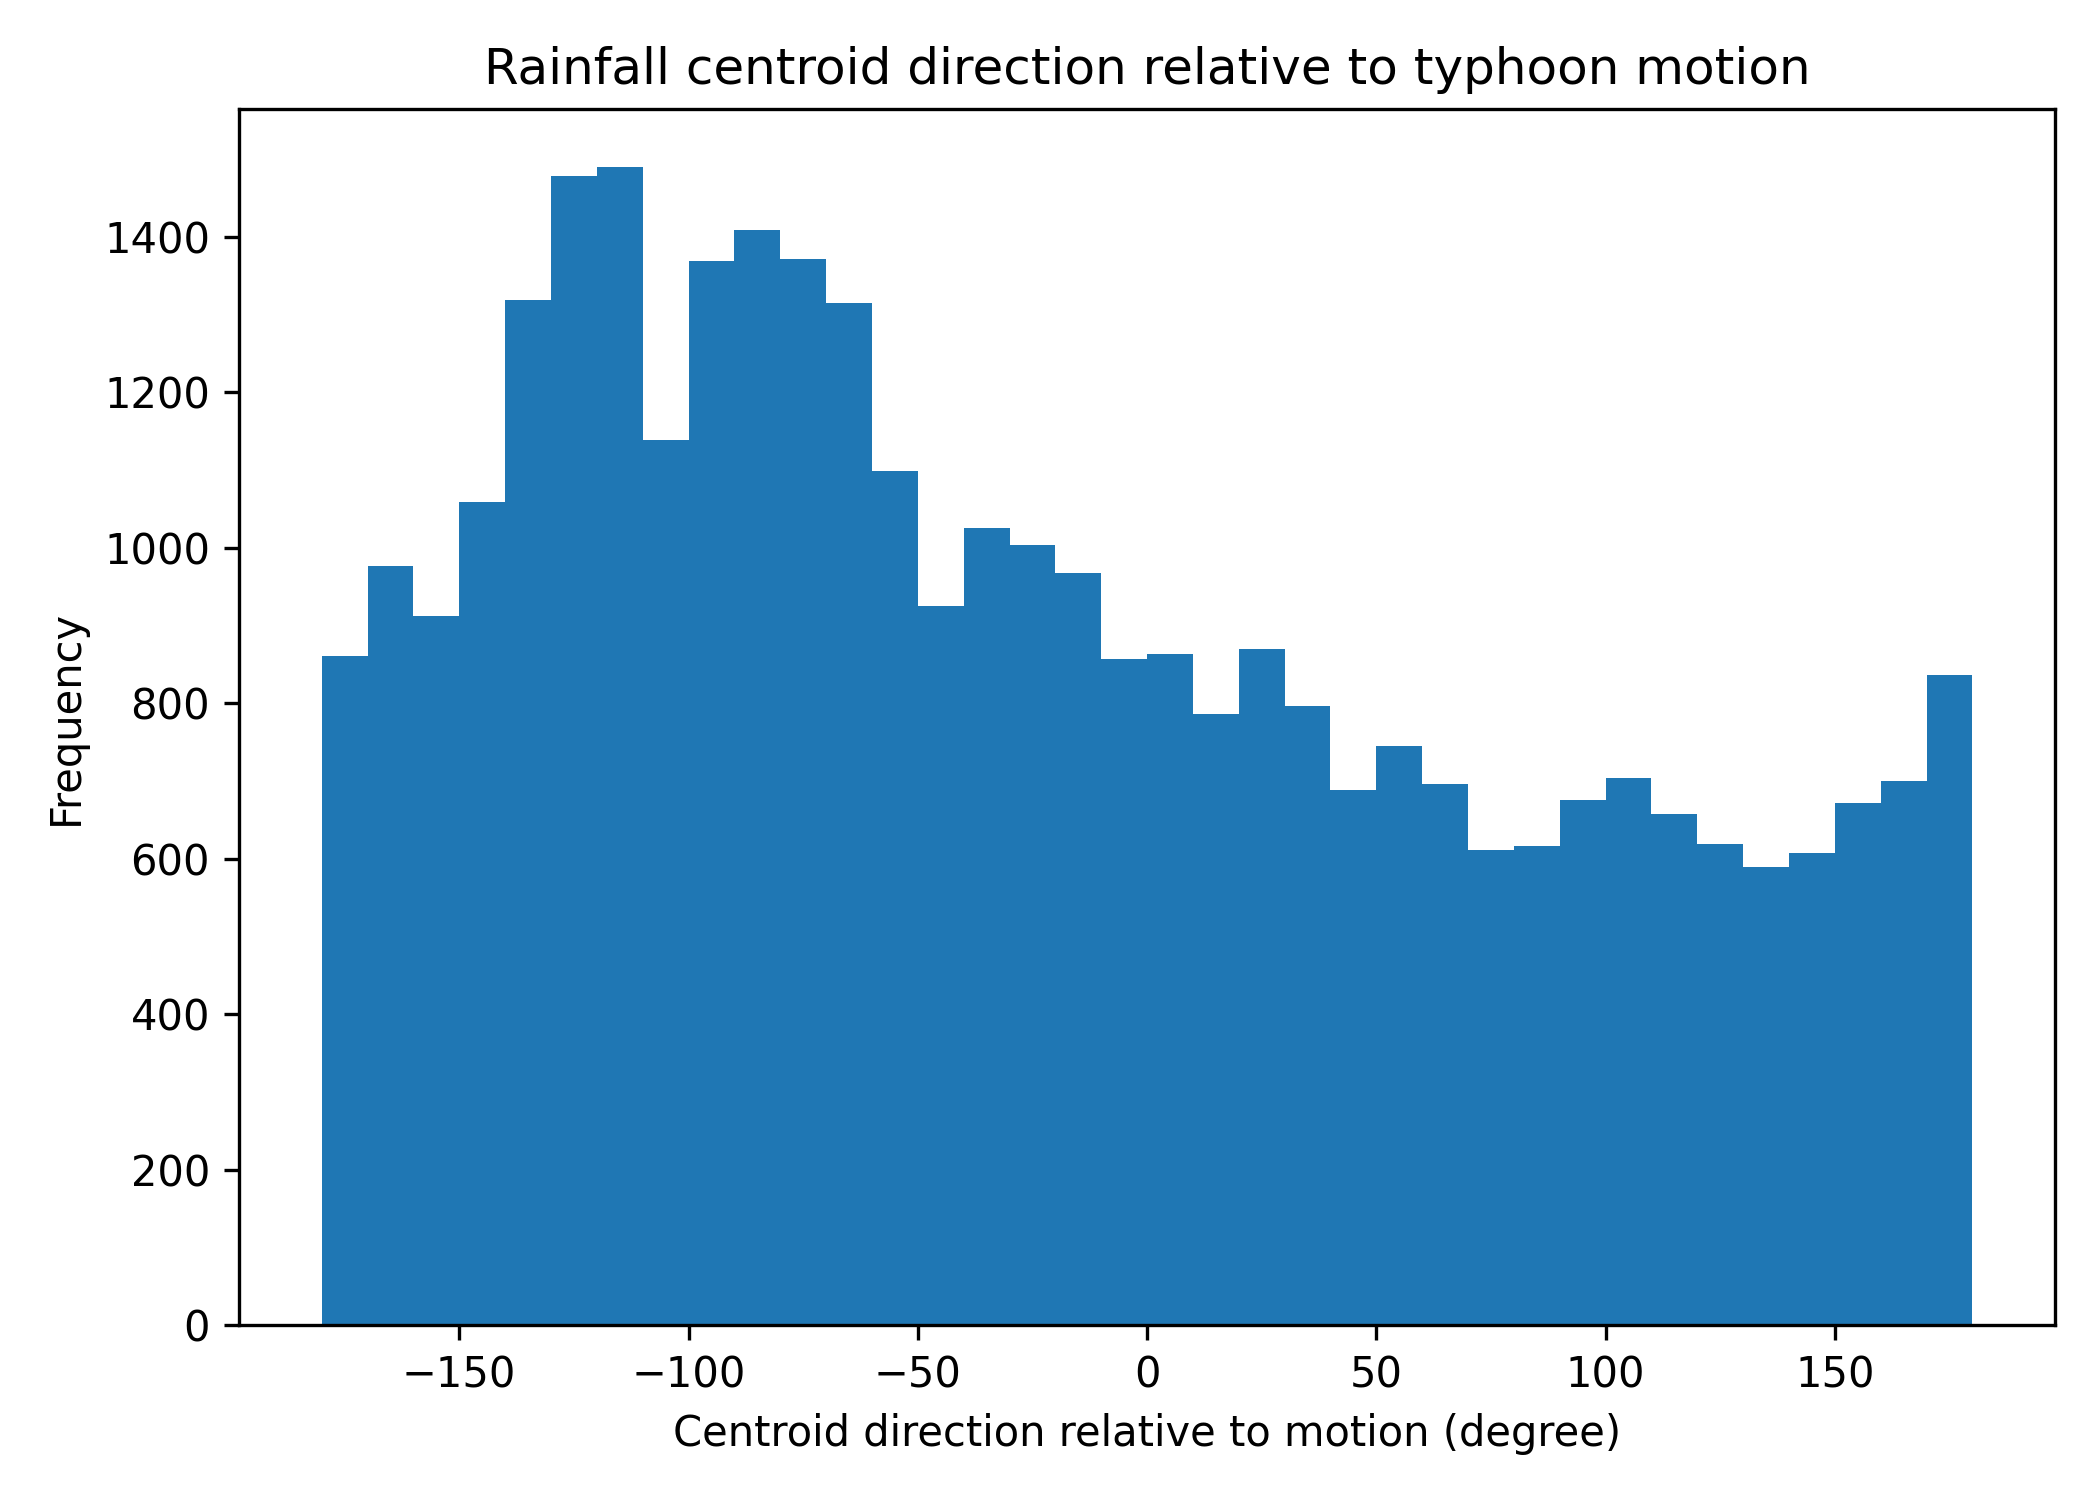
\includegraphics[width=0.72\textwidth]{06_centroid_relative_to_motion_hist.png}
    \caption{降水质心方向相对于台风移动方向的分布}
    \label{fig:centroid_motion_hist_problem1}
\end{figure}

\subsubsection{台风相对运动坐标系下的降水偏向特征}

为进一步检验降水分布是否相对于台风移动方向存在系统性偏向，本文基于逐格旋转后的台风相对运动坐标系，统计了前后、左右及四象限降水比例。结果显示，历史样本中降水整体更偏向台风移动前方和左侧。所有有效样本中，前方降水比例均值为$54.1\%$，后方为$45.9\%$；左侧降水比例均值为$55.0\%$，右侧为$45.0\%$。对应地，前后非对称性$A_{FB}$的均值和中位数分别为$0.083$和$0.056$，左右非对称性$A_{LR}$的均值和中位数分别为$0.100$和$0.138$。

\begin{figure}[htbp]
    \centering
    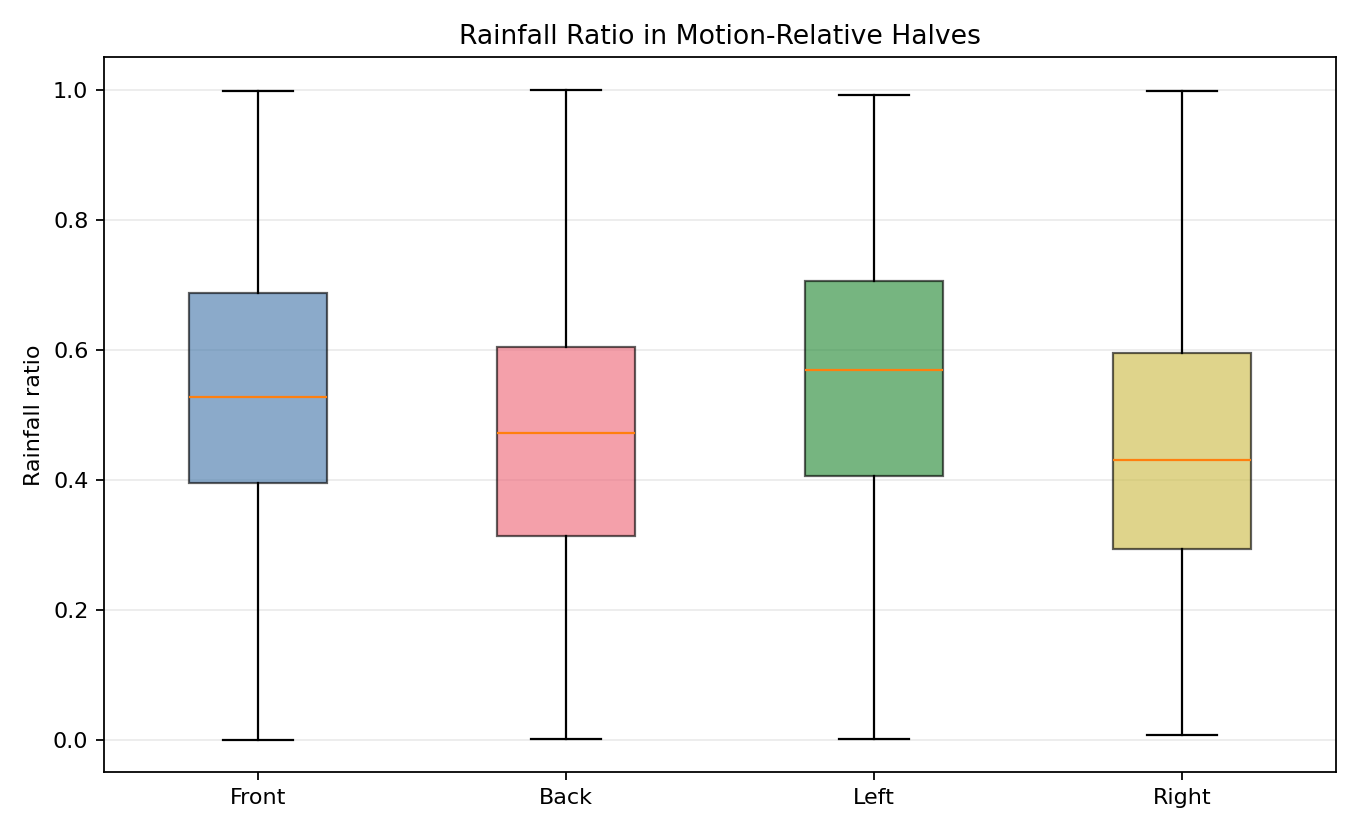
\includegraphics[width=0.78\textwidth]{motion_front_back_left_right_boxplot.png}
    \caption{台风相对运动坐标系下前后、左右降水比例分布}
    \label{fig:motion_fb_lr_ratio_problem1}
\end{figure}

进一步考察四象限降水比例可发现，平均和中位数最大的均为前左象限。四象限平均比例分别为：前左象限$30.2\%$、前右象限$24.0\%$、后左象限$24.8\%$、后右象限$21.0\%$。这说明台风降水并不是在台风中心周围均匀分布，而是相对于移动方向存在明显的前侧和左侧偏向。

\begin{figure}[htbp]
    \centering
    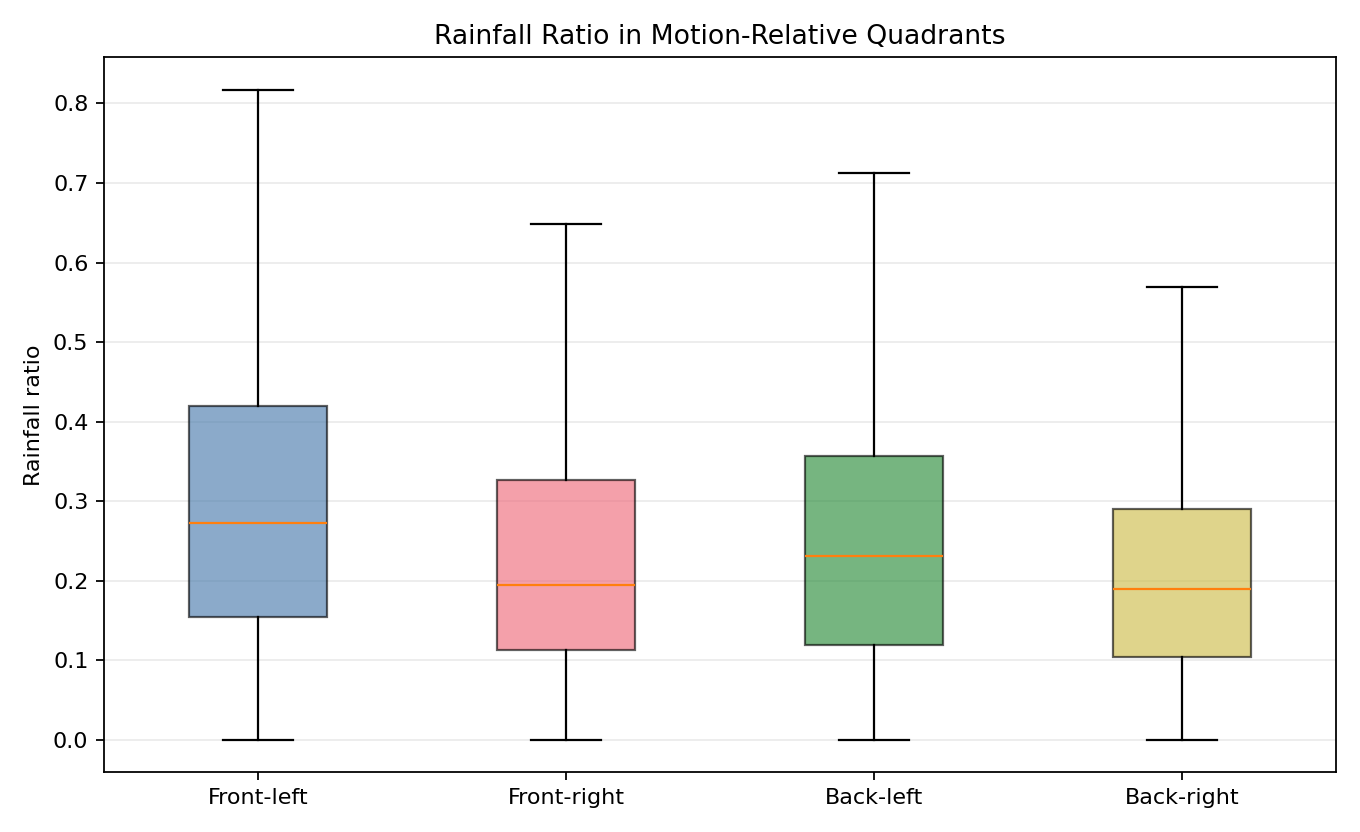
\includegraphics[width=0.78\textwidth]{motion_quadrant_ratio_boxplot.png}
    \caption{台风相对运动坐标系下四象限降水比例分布}
    \label{fig:motion_quadrant_ratio_problem1}
\end{figure}

从强降水面积看，$10\ \mathrm{mm/hr}$以上强降水面积在台风前方和左侧也更大。其中，前方强降水面积中位数为$17158.9\ \mathrm{km^2}$，后方为$11962.6\ \mathrm{km^2}$；左侧强降水面积中位数为$17761.9\ \mathrm{km^2}$，右侧为$11591.7\ \mathrm{km^2}$。这进一步表明，台风运动方向不仅影响降水总量分布，也会影响强降水区域的位置。

\begin{figure}[htbp]
    \centering
    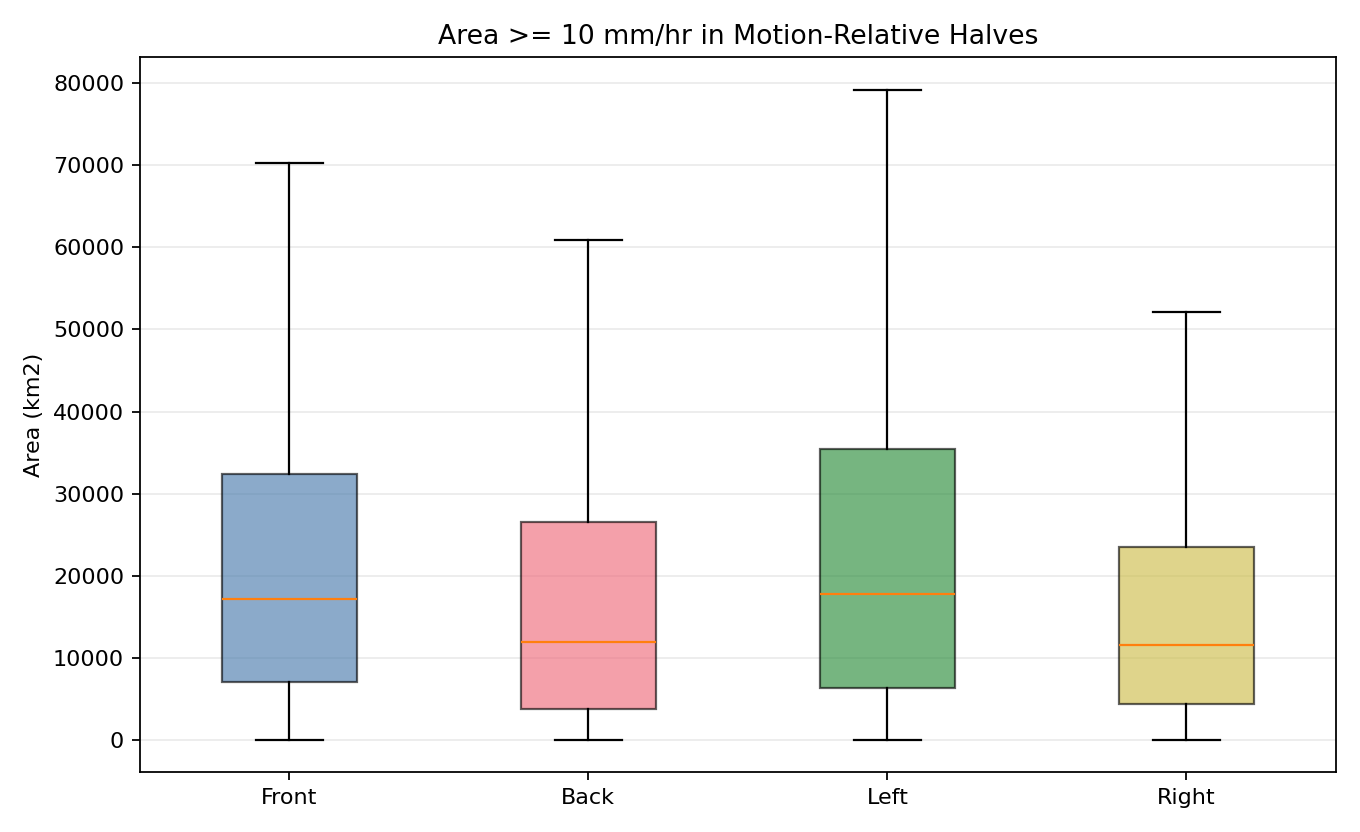
\includegraphics[width=0.78\textwidth]{motion_area10_boxplot.png}
    \caption{台风相对运动坐标系下$10\ \mathrm{mm/hr}$以上强降水面积分布}
    \label{fig:motion_area10_problem1}
\end{figure}

此外，雨带主轴相对于台风移动方向的夹角均值和中位数分别约为$44.9^\circ$和$44.8^\circ$，说明降水带通常并非严格沿台风移动方向伸展，而是与移动方向存在一定斜交角。这一结果表明，雨带结构受到台风移动方向、环境风场和水汽输送方向共同调制。

\begin{figure}[htbp]
    \centering
    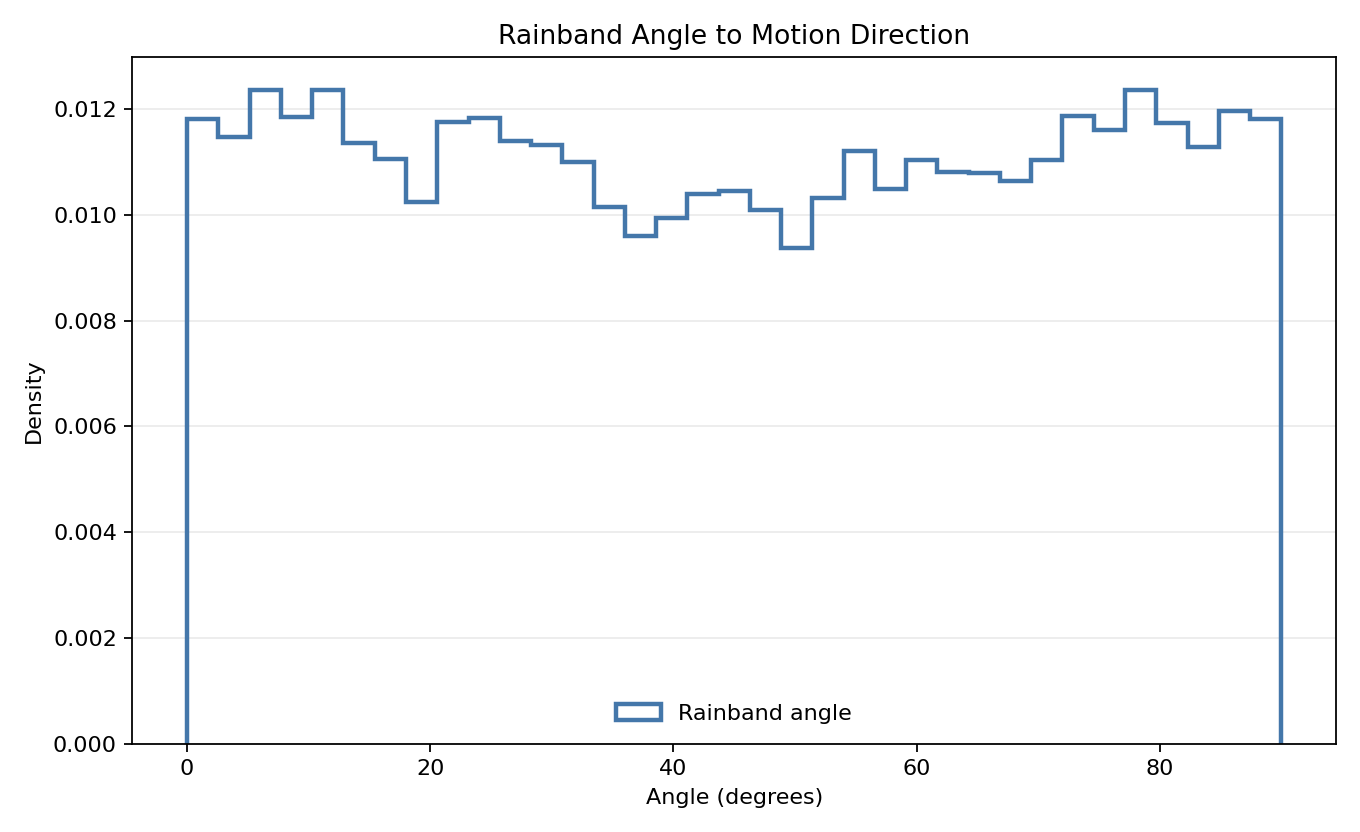
\includegraphics[width=0.72\textwidth]{rainband_angle_to_motion_hist.png}
    \caption{雨带主轴相对于台风移动方向的夹角分布}
    \label{fig:rainband_motion_angle_problem1}
\end{figure}

表\ref{tab:motion_relative_stats_problem1}汇总了台风相对运动坐标系下的主要降水结构指标。

\begin{table}[htbp]
    \centering
    \caption{台风相对运动坐标系下降水结构指标统计}
    \label{tab:motion_relative_stats_problem1}
    \begin{tabular}{lcc}
        \hline
        指标 & 均值 & 中位数 \\
        \hline
        前方降水比例 & 0.541 & -- \\
        后方降水比例 & 0.459 & -- \\
        左侧降水比例 & 0.550 & -- \\
        右侧降水比例 & 0.450 & -- \\
        前后非对称性$A_{FB}$ & 0.083 & 0.056 \\
        左右非对称性$A_{LR}$ & 0.100 & 0.138 \\
        前左象限比例 & 0.302 & -- \\
        前右象限比例 & 0.240 & -- \\
        后左象限比例 & 0.248 & -- \\
        后右象限比例 & 0.210 & -- \\
        雨带相对运动方向夹角 & $44.9^\circ$ & $44.8^\circ$ \\
        \hline
    \end{tabular}
\end{table}

\subsubsection{季节背景与海陆因素的调制作用}

从随机森林重要性看，月份周期变量在多个目标变量中具有较高贡献。例如，$month\_cos$在$rain\_p95$、$rain\_area\_10\_km^2$、$centroid\_offset$和$anisotropy$模型中均排名靠前。这说明台风降水结构不仅受台风自身路径和强度影响，还受到季节背景环流和水汽供应条件的调制。不同月份西太平洋水汽输送、季风背景和副热带高压位置存在差异，这些因素会改变台风降水带的组织形态和强降水范围。

海陆和距岸因素也在多个模型中具有一定贡献。例如，$track\_signed\_coast\_dist\_km$在强降水等效半径、降水质心偏移和雨带各向异性模型中均进入前十；近岸影响指数$coast\_influence\_exp$也对降水质心偏移具有一定贡献。这说明海陆热力差异、陆面摩擦和地形抬升会调制台风降水空间分布。但与台风强度、移动方向和季节背景相比，海陆因素更多体现为调制因子，而非唯一主控因子。

\subsection{主要影响因素综合排序}

为了进一步比较不同目标变量的主控因子，本文整理随机森林置换重要性排名前五的变量，如表\ref{tab:rf_top_factors_problem1}所示。

\begin{table}[htbp]
    \centering
    \caption{不同降水分布特征的主要影响因素}
    \label{tab:rf_top_factors_problem1}
    \begin{tabular}{p{0.25\textwidth}p{0.62\textwidth}c}
        \hline
        响应变量 & 随机森林重要性前五变量 & 测试集$R^2$ \\
        \hline
        $rain\_max$ & 移动方向正弦、最大风速、移动速度、月份余弦、气压亏损 & 0.406 \\
        $rain\_p95$ & 移动方向正弦、月份余弦、综合强度指数、移动方向余弦、移动速度 & 0.648 \\
        $rain\_area\_10\_km^2$ & 移动方向正弦、最大风速、月份余弦、气压亏损、移动方向余弦 & 0.584 \\
        强降水等效半径 & 最大风速、移动方向正弦、月份余弦、有符号距岸距离、中心气压 & 0.642 \\
        降水质心偏移 & 移动方向正弦、移动速度、月份余弦、综合强度指数、移动方向余弦 & 0.672 \\
        雨带各向异性 & 移动方向正弦、移动速度、月份余弦、移动方向余弦、月份正弦 & 0.636 \\
        \hline
    \end{tabular}
\end{table}

由表\ref{tab:rf_top_factors_problem1}可知，移动方向正弦在所有主要目标变量中均排名靠前，说明台风降水分布对台风路径方向具有显著依赖。强度相关变量主要控制降水强度和强降水范围；移动速度和移动方向主要控制降水质心偏移与雨带形态；月份周期变量在多个目标变量中均有贡献，表明季节背景不可忽略；距岸距离对强降水等效半径和雨带结构具有一定调制作用。进一步在台风相对运动坐标系下计算前后、左右和四象限降水比例后，可以发现历史台风降水总体偏向运动前方和左侧，这进一步说明降水非对称性并非固定的东西南北偏向，而是与台风动力过程和移动方向密切相关。

\subsection{模型检验与进一步讨论}

为检验模型是否仅仅拟合同一台风事件内部的连续演变，本文设置两种验证方式。第一种为普通随机划分，即随机抽取半小时时次样本进入训练集和测试集；第二种为按台风事件分组划分，即以$track\_event\_uid$为分组单位，保证同一场台风不会同时出现在训练集和测试集中。前者主要检验模型对同一台风过程内部降水演变规律的解释能力，后者则更接近对未知台风事件的外推检验。两种验证方式的结果如表\ref{tab:random_vs_group_validation_problem1}所示。

\begin{table}[htbp]
    \centering
    \caption{普通随机划分与按台风事件分组划分的模型验证结果对比}
    \label{tab:random_vs_group_validation_problem1}
    \small
    \begin{tabular}{lrrrr}
        \hline
        指标 & 随机划分$R^2$ & 按台风分组$R^2$ & $R^2$下降 & MAE增幅/\% \\
        \hline
        最大降水强度 & 0.417 & -0.072 & 0.488 & 47.2 \\
        95分位降水强度 & 0.649 & 0.036 & 0.613 & 86.3 \\
        强降水面积 & 0.586 & -0.015 & 0.601 & 75.3 \\
        强降水等效半径 & 0.645 & 0.014 & 0.631 & 83.4 \\
        降水中心偏移距离 & 0.674 & -0.117 & 0.791 & 88.5 \\
        雨带各向异性 & 0.640 & -0.032 & 0.671 & 72.4 \\
        \hline
    \end{tabular}
\end{table}

由表\ref{tab:random_vs_group_validation_problem1}可见，在普通随机划分下，增强随机森林模型对95分位降水强度、强降水面积、强降水等效半径、降水中心偏移距离和雨带各向异性均具有较高解释能力，测试集$R^2$大多在0.58以上。这说明路径、强度、移动方向、季节背景和海陆因素能够较好刻画同一台风过程内部的降水结构演变。

然而，在按台风事件分组划分后，测试集$R^2$明显下降，其中多个目标变量的$R^2$接近0或为负，MAE也显著增加。这表明当测试集为模型从未见过的台风事件时，仅依赖路径、强度、近岸和时间背景变量难以稳定外推逐时降水结构。换言之，不同台风事件之间存在显著个体差异，台风降水还受到水汽输送、垂直风切变、背景环流、海温和地形抬升等未显式引入变量的影响。

该检验结果具有重要意义：问题一中的随机森林模型更适合用于解释历史台风过程中路径、强度和环境因素对降水分布的影响规律，而不宜直接作为问题二中KONG-REY和MAN-YI的逐格降水生成模型。因此，在后续问题二中，本文不采用简单监督回归直接预测目标台风降水场，而采用“相似历史时次筛选—台风相对坐标下降水模板迁移—强度、极端分位数与近岸因子校准”的生成思路。同时，由于问题一结果表明降水结构具有明显的台风相对运动方向偏向，后续模板迁移将在台风相对运动坐标系下进行，以避免直接在经纬度坐标中比较不同路径方向台风导致的结构错位。

需要特别说明的是，问题一中提取的降水结构特征变量，如
$\mathrm{rain\_p95}$、$\mathrm{rain\_area\_10\_km^2}$、$\mathrm{centroid\_offset}$、$\mathrm{anisotropy}$，
以及前后向、左右向降水比例等，均由GPM降水场计算得到。然而，由于台风KONG-REY和MAN-YI在GPM数据集中不存在对应的降水记录，上述降水结构变量在问题二中无法作为目标台风的输入特征使用。因此，这些变量仅用于历史样本的输出指标描述、生成结果的校准目标以及模型合理性的检验依据。问题二的模型输入仅选取目标台风可直接获取或可由路径数据派生的变量，包括路径特征（位置、移动速度与方向）、强度特征（气压、风速）、时间季节特征，以及环境特征（海陆分布、近岸距离等）。

综上，模型检验表明：本文所建问题一模型能够较好解释同一台风过程内部的降水时空演变规律，并能识别影响降水强度、范围、质心偏移和雨带形态的主要因素；但对于完全未知的台风事件，单纯依靠路径和强度变量进行逐时外推存在明显局限。因此，问题一模型在全文中的定位是“关系解释与特征筛选模型”，其结论为问题二中相似样本筛选、降水模板迁移和生成结果校准提供依据。


\subsection{问题一结论}

综合以上分析，得到如下结论：

\begin{enumerate}
    \item 台风强度是影响降水强度和强降水范围的主控因子。中心气压越低、气压亏损越大、最大风速越强，P95降水强度和强降水面积越大。
    \item 台风移动方向和移动速度显著影响降水空间结构。移动方向正弦和余弦特征在多个模型中排名靠前，说明降水质心偏移、非对称性和雨带形态均具有明显路径方向依赖。
    \item 在台风相对运动坐标系下，降水总体偏向移动前方和左侧。前左象限为平均降水比例最大的区域，且$10\ \mathrm{mm/hr}$以上强降水面积也主要集中在前方和左侧，说明台风降水非对称性与台风移动方向密切相关。
    \item 台风增强或减弱过程会改变降水非对称性。风速变化率和气压变化率与东西、南北非对称性存在较明显相关，说明降水偏向不仅由当前强度决定，还与台风演变趋势有关。
    \item 季节背景是不可忽略的调制因子。月份周期变量在多个模型中具有较高重要性，说明水汽供应和背景环流条件会影响台风降水强度、范围和雨带形态。
    \item 海陆与距岸因素对降水结构具有调制作用。距岸距离和近岸影响指数对强降水范围、降水质心偏移和雨带各向异性具有一定贡献，但其作用通常弱于强度、移动方向和季节背景。
\end{enumerate}

\section{问题二模型的建立与求解}

问题二要求在 KONG-REY 和 MAN-YI 两场台风没有 GPM 降水记录的条件下，依据历史台风的“路径--强度--环境--降水”关系生成其可能的半小时降水时空分布。因此，本问不是普通的标量预测问题，而是一个条件降水场生成问题。本文将生成过程分解为七个环节：历史半小时样本库构建、目标台风安全输入构造、历史相似时次检索、台风相对坐标模板迁移、EOF/PCA 大尺度结构修正、极端分位数校准和历史台风伪缺失验证。最终以极端校准后的降水场作为 KONG-REY 与 MAN-YI 的可能降水分布结果。

\subsection{建模思路与安全输入说明}

由于 KONG-REY 和 MAN-YI 在 GPM 降水数据集中没有真实降水记录，模型输入必须严格限定为目标台风在生成时可获得的信息，包括路径、强度、移动、时间和海陆环境特征。本文将由历史 GPM 降水场计算得到的降水指标仅作为历史标签、模板校准目标和验证指标，而不作为目标台风输入，以避免数据泄漏。

对任一目标半小时时刻 $t$，构造安全输入向量
\begin{equation}
\boldsymbol{X}_t=
\left[
\varphi_t,\lambda_t,WND_t,PRES_t,I_t,U_t,
\sin \alpha_t,\cos \alpha_t,
\Delta WND_t,\Delta PRES_t,
L_t,d_t,
\sin m_t,\cos m_t,p_t
\right],
\end{equation}
其中，$\varphi_t,\lambda_t$ 分别为台风中心纬度和经度，$WND_t$ 为最大风速字段，$PRES_t$ 为中心最低气压，$I_t$ 为强度等级，$U_t$ 为移动速度，$\alpha_t$ 为移动方向，$\Delta WND_t,\Delta PRES_t$ 为强度变化率，$L_t$ 为是否登陆或陆地标记，$d_t$ 为距岸距离，$m_t$ 为月份，$p_t$ 为生命周期进程。由于路径数据中 OWD 字段缺失，本文不使用 OWD。

历史半小时样本库共包含 $32842$ 个历史时次、$88$ 个字段，每行对应一个历史台风的一个半小时时刻。问题一中完成路径匹配的 GPM 半小时时次数为 $33420$；问题二构建历史模板库时，为避免目标台风降水信息泄漏，将 2024 年目标台风名称或目标时间窗对应的 $578$ 个 GPM 半小时时次从历史库中排除，剩余样本全部成功入库，因此最终得到 $32842$ 个可用于相似检索和模板迁移的历史半小时时次。目标台风安全输入表共包含 $974$ 个半小时时刻，其中 KONG-REY 包含 $421$ 个时刻，时间范围为 2024-10-24 18:00:00 至 2024-11-02 12:00:00；MAN-YI 包含 $553$ 个时刻，时间范围为 2024-11-08 12:00:00 至 2024-11-20 00:00:00。

需要特别说明的是，以下由 GPM 降水场计算得到的字段均不参与目标台风输入和相似检索：
\begin{equation}
\texttt{rain\_*},\quad
\texttt{centroid\_*},\quad
\texttt{quad\_*},\quad
\texttt{anisotropy},\quad
\texttt{rain\_radius\_*},\quad
\texttt{rain\_band\_width}.
\end{equation}
这些字段只用于历史样本描述、极端分位数校准和伪缺失验证。由于本轮数据中 \texttt{landfrac/elev/terrain} 类变量全缺失，实际检索时主要使用 \texttt{is\_land}、\texttt{signed\_coast\_dist\_km} 和 \texttt{coast\_dist\_km} 表征海陆环境。

\subsection{历史相似样本检索模型}

\subsubsection{安全特征标准化}

对每个目标时刻 $t$，本文从历史样本库中检索与其路径、强度、移动、季节和海陆环境最相似的历史半小时时次。所有连续变量均使用历史库均值与标准差进行标准化：
\begin{equation}
z_j(x)=\frac{x-\mu_j}{\sigma_j+\varepsilon},
\end{equation}
其中 $\mu_j,\sigma_j$ 分别为历史库中特征 $j$ 的均值和标准差，$\varepsilon$ 为防止除零的小常数。移动方向采用 $\sin \alpha$ 和 $\cos \alpha$ 表示，避免角度循环造成的距离误差。

\subsubsection{分量距离与总距离}

本文将相似距离分解为六个部分：
\begin{align}
D_{\mathrm{track}} &= \operatorname{mean}\left[
\Delta z(\varphi)^2,\Delta z(\lambda)^2
\right],\\
D_{\mathrm{intensity}} &= \operatorname{mean}\left[
\Delta z(WND)^2,\Delta z(PRES)^2,\Delta z(I)^2
\right],\\
D_{\mathrm{motion}} &= \operatorname{mean}\left[
\Delta z(U)^2,\Delta z(\sin\alpha)^2,\Delta z(\cos\alpha)^2,
\Delta z(\Delta WND)^2,\Delta z(\Delta PRES)^2
\right],\\
D_{\mathrm{env}} &= \operatorname{mean}\left[
\Delta z(L)^2,\Delta z(d)^2
\right],\\
D_{\mathrm{time}} &= \operatorname{mean}\left[
\Delta z(\sin m)^2,\Delta z(\cos m)^2
\right],\\
D_{\mathrm{life}} &= \Delta z(p)^2.
\end{align}
总距离定义为
\begin{equation}
D(t,s)=
1.0D_{\mathrm{track}}
+1.5D_{\mathrm{intensity}}
+1.2D_{\mathrm{motion}}
+1.2D_{\mathrm{env}}
+0.8D_{\mathrm{time}}
+0.8D_{\mathrm{life}},
\end{equation}
其中 $s$ 表示历史候选时次。若某类特征整体缺失，则自动跳过该特征，并对该分量按实际可用特征数取平均，避免某一类变量因字段数较多而天然占据更高权重。

上述距离分量权重并非任意设定，而是依据问题一中变量解释结果和台风降水物理含义确定。问题一的结果表明，强度变量（WND、PRES）对 $R_{95}$、$R_{99}$ 以及强降水面积具有稳定影响，因此本文对强度分量赋予较高权重 $1.5$；移动速度和移动方向直接影响降水质心偏移、前后/左右非对称性和雨带各向异性，因此移动分量权重设为 $1.2$，略高于单纯路径位置分量；近岸距离和是否登陆等海陆环境变量会改变台风降水的空间范围和雨带形态，因此环境分量同样设为 $1.2$；月份变量主要反映背景水汽条件和季节环流差异，作为辅助筛选因素，权重设为 $0.8$；生命周期进程用于避免将台风初生阶段、成熟阶段和减弱阶段错误匹配，也作为辅助约束，权重设为 $0.8$。由此，本文相似距离既强调强度和移动结构对降水场的主导作用，又保留季节和生命周期对历史样本匹配的修正作用。进一步地，表 \ref{tab:p2_sensitivity_result} 的敏感性分析表明，关键参数扰动下模型性能未出现明显突变，说明该权重设置具有一定鲁棒性。

对每个目标时刻，选取距离最小的 $K=20$ 个历史时次作为相似样本。为避免相似样本被某一场历史台风垄断，设置同一历史事件在单个目标时刻的 Top-$K$ 中最多出现 $3$ 次。最终每个目标时刻的 Top-$K$ 中唯一历史台风事件数均值为 $7.165$，最小值为 $7$，说明相似模板来源具有一定多样性。

\subsubsection{相似权重}

对选出的 Top-$K$ 历史样本，采用 softmax 距离权重：
\begin{equation}
\omega_j(t)=
\frac{\exp[-D(t,s_j)/\tau_t]}
{\sum_{k=1}^{K}\exp[-D(t,s_k)/\tau_t]},
\end{equation}
其中 $\tau_t$ 取该目标时刻 Top-$K$ 距离的中位数。最终得到 $974\times 20=19480$ 条目标--历史相似样本匹配记录，每个目标时刻均有 $20$ 个历史相似样本，且权重和为 $1$。相似距离的中位数为 $1.156$，$95\%$ 分位数为 $2.345$。Top-$K$ 历史样本中不包含 KONG-REY、MAN-YI 及其目标时间窗样本。

\subsection{\texorpdfstring{storm-relative}{storm-relative} 模板迁移生成模型}

\subsubsection{台风相对运动坐标系}

直接在经纬度坐标下比较不同台风的降水场会混淆移动方向差异。为统一不同台风的雨带结构，本文将历史 GPM 降水场转换到台风相对运动坐标系。设台风中心为 $(\lambda_c,\varphi_c)$，原始相对坐标中的 $x$ 表示向东距离，$y$ 表示向北距离：
\begin{equation}
x=111.32\cos(\varphi_c)(\lambda-\lambda_c),\qquad
y=111.32(\varphi-\varphi_c).
\end{equation}
设 $\alpha$ 为台风移动方向角，$0^\circ$ 表示正北，$90^\circ$ 表示正东。定义
\begin{equation}
x_f=x\sin\alpha+y\cos\alpha,\qquad
y_l=-x\cos\alpha+y\sin\alpha,
\end{equation}
其中 $x_f>0$ 表示台风移动前方，$y_l>0$ 表示移动方向左侧。本文采用统一相对坐标网格：
\begin{equation}
x_f,y_l\in[-1000,1000]\ \mathrm{km},\qquad
201\times 201.
\end{equation}

\subsubsection{Top-$K$ 模板加权生成}

对每个目标时刻 $t$，读取其 Top-$K$ 历史样本的 GPM 降水场 $R_{s_j}$，重采样到上述台风相对运动坐标网格。为减弱极端值对加权平均的影响，并保证雨场非负，本文在 $\log(1+R)$ 空间进行模板迁移：
\begin{equation}
G_t^{(0)}(x_f,y_l)
=
\sum_{j=1}^{K}\omega_j(t)\log\left[1+R_{s_j}(x_f,y_l)\right],
\end{equation}
\begin{equation}
R_t^{(0)}(x_f,y_l)
=
\exp\left(G_t^{(0)}(x_f,y_l)\right)-1.
\end{equation}
这里 $R_t^{(0)}$ 为初始生成场，单位为 \(\mathrm{mm/hr}\)。若计算半小时累计量，则使用 $0.5R_t^{(0)}$。

初始场共生成 $974$ 个半小时时次，数组维度为 $(974,201,201)$，没有 NaN、Inf、负值或全零场。其最大格点降水 $R_{\max}$ 的中位数、$95\%$ 分位数和最大值分别为 $8.178$、$23.329$ 和 $29.443\ \mathrm{mm/hr}$。但初始场相对于 Top-$K$ 历史样本加权最大值的比值中位数仅为 $0.184$，表明 $\log(1+R)$ 加权平均虽能较好保留大尺度雨区形态，但会明显平滑局地极端降水。因此后续需要引入极端分位数校准。

\subsection{EOF/PCA 大尺度结构修正}

\subsubsection{EOF/PCA 空间模态分解}

为增强生成雨场的大尺度结构稳定性和可解释性，本文进一步对历史相似模板进行 EOF/PCA 分解。选取目标相关的唯一 Top-$K$ 历史模板作为训练集，共 $2166$ 个历史相似降水模板。对每个模板取
\begin{equation}
G_s(x_f,y_l)=\log\left[1+R_s(x_f,y_l)\right],
\end{equation}
并在 $\log(1+R)$ 空间进行 PCA 分解：
\begin{equation}
G_s(x_f,y_l)
\approx
\mu(x_f,y_l)+
\sum_{k=1}^{K_{\mathrm{EOF}}}a_{k,s}\phi_k(x_f,y_l),
\end{equation}
其中 $\mu$ 为历史平均场，$\phi_k$ 为第 $k$ 个 EOF 空间模态，$a_{k,s}$ 为对应系数。本文取 $K_{\mathrm{EOF}}=20$。前五个 EOF 模态的解释率分别为
\[
0.1037,\quad 0.0850,\quad 0.0516,\quad 0.0447,\quad 0.0304,
\]
20 个 EOF 模态累计解释率为 $0.5007$。这说明 EOF/PCA 模态主要刻画台风降水的大尺度空间结构，而不试图完全还原局地极端雨强。

\subsubsection{目标初始场投影与 EOF 重构}

对目标台风的初始场 $R_t^{(0)}$，令
\begin{equation}
G_t^{(0)}=\log\left(1+R_t^{(0)}\right).
\end{equation}
将其投影到 EOF 空间，得到目标 EOF 系数：
\begin{equation}
\hat a_{k,t}
=
\left\langle
G_t^{(0)}-\mu,\phi_k
\right\rangle.
\end{equation}
由此得到 EOF 重构场：
\begin{equation}
G_t^{\mathrm{EOF}}
=
\mu+\sum_{k=1}^{K_{\mathrm{EOF}}}\hat a_{k,t}\phi_k,
\end{equation}
\begin{equation}
R_t^{\mathrm{EOF}}
=
\exp\left(G_t^{\mathrm{EOF}}\right)-1.
\end{equation}

由于 EOF/PCA 重构也可能削弱局地极端降水，本文不直接以 $R_t^{\mathrm{EOF}}$ 作为生成结果，而采用保守融合：
\begin{equation}
R_t^{\mathrm{blend}}
=
(1-\beta)R_t^{(0)}+\beta R_t^{\mathrm{EOF}},
\qquad \beta=0.3.
\end{equation}
其中 $R_t^{\mathrm{blend}}$ 为大尺度结构修正场。结果表明，$R_t^{\mathrm{blend}}$ 与 $R_t^{(0)}$ 的空间相关系数中位数为 $0.995$，$95\%$ 分位数为 $0.998$，说明 EOF/PCA 修正没有破坏初始模板场的主要结构。$R_t^{\mathrm{blend}}$ 相对于初始场最大雨强的比值中位数为 $0.884$，说明 $\beta=0.3$ 的融合方式较为保守。

\subsection{极端分位数校准}

\subsubsection{校准与验证目标构造}

由上一节可知，模板加权和 EOF/PCA 修正均可能削弱局地极端降水。为使生成结果更符合历史相似台风的极端分布，本文以 Top-$K$ 历史样本的 P95 和 P99 作为直接校准目标，同时计算 $A_{10}$ 和 $A_{20}$ 作为强降水面积合理性的辅助检验指标。由于强降水面积与雨场空间结构密切相关，若直接强制匹配面积，可能破坏模板迁移得到的雨带形态，因此本文不对 $A_{10}$ 和 $A_{20}$ 做硬约束，而在校准后检验其误差变化。对每个目标时刻 $t$，计算：
\begin{align}
T_{95,t} &= \sum_{j=1}^{K}\omega_j(t)Q_{0.95}(R_{s_j}),\\
T_{99,t} &= \sum_{j=1}^{K}\omega_j(t)Q_{0.99}(R_{s_j}),\\
T_{\max,t} &= \sum_{j=1}^{K}\omega_j(t)\max(R_{s_j}),\\
T_{A10,t} &= \sum_{j=1}^{K}\omega_j(t)A_{10}(R_{s_j}),\\
T_{A20,t} &= \sum_{j=1}^{K}\omega_j(t)A_{20}(R_{s_j}),
\end{align}
其中 $Q_{0.95}$ 和 $Q_{0.99}$ 分别表示 $95\%$ 和 $99\%$ 分位数，$A_{10},A_{20}$ 分别表示降水强度超过 $10\ \mathrm{mm/hr}$ 和 $20\ \mathrm{mm/hr}$ 的面积。$T_{95,t}$ 和 $T_{99,t}$ 用于尾部增强的直接分位数校准，$T_{\max,t}$ 用于约束极端尾部的合理量级，$T_{A10,t}$ 和 $T_{A20,t}$ 则作为强降水面积验证目标。为降低个别异常历史样本影响，对 Top-$K$ 历史极端指标先进行温和 winsorize 处理，再计算加权目标。

\subsubsection{尾部增强校准}

本文不采用简单全场乘法校准，因为整体放大会同时放大弱降水区，导致雨区面积虚高。设结构底图为 $R_t^{\mathrm{blend}}$，其分位数为 $q_{90},q_{95},q_{99}$。本文采用分段尾部增强函数：
\begin{equation}
w_{\mathrm{tail}}(r)
=
\mathrm{clip}
\left(
\frac{r-q_{90}}{q_{99}-q_{90}+\varepsilon},0,1
\right),
\end{equation}
对中高雨强区进行 P95 校准：
\begin{equation}
R_1
=
R_t^{\mathrm{blend}}
\left[
1+w_{\mathrm{tail}}(R_t^{\mathrm{blend}})
\left(
\frac{T_{95,t}}{q_{95}+\varepsilon}-1
\right)
\right].
\end{equation}
随后对 $R_1\ge Q_{0.99}(R_1)$ 的极端尾部进行进一步增强，使 P99 和最大雨强接近历史相似目标。最终得到校准场 $R_t^{\mathrm{cal}}$。校准过程中设置非负约束和物理上限：
\begin{equation}
0\le R_t^{\mathrm{cal}}\le
\min\left(120,\ 1.25\max_{j\in\mathrm{Top}K}\max(R_{s_j})\right).
\end{equation}
本次生成中没有出现物理上限截断。

\subsubsection{校准效果}

校准前后极端指标对比如表 \ref{tab:p2_calibration_effect} 所示。可以看出，校准前的 blended 场最大雨强明显偏低；校准后，P95 和 P99 与历史相似样本给出的目标分布基本一致，最大格点雨强也提升到合理量级。

\begin{table}[H]
\centering
\caption{极端分位数校准前后指标对比}
\label{tab:p2_calibration_effect}
\resizebox{\textwidth}{!}{
\begin{tabular}{lccc}
\toprule
指标 & 目标值 P50/P95/max & blended 场 P50/P95/max & calibrated 场 P50/P95/max \\
\midrule
$R_{\max}$ / mm$\cdot$h$^{-1}$ 
& 44.781 / 54.918 / 59.325
& 7.186 / 21.554 / 26.553
& 35.931 / 49.728 / 54.405 \\
$R_{95}$ / mm$\cdot$h$^{-1}$ 
& 2.728 / 4.053 / 4.993
& -- 
& 2.722 / 4.053 / 4.993 \\
$R_{99}$ / mm$\cdot$h$^{-1}$ 
& 9.926 / 14.242 / 17.141
& -- 
& 9.041 / 14.238 / 17.141 \\
\bottomrule
\end{tabular}}
\end{table}

校准后 $R_{95}$ 和 $R_{99}$ 相对于目标值的比值中位数均为 $1.000$，说明极端分位数目标得到了有效匹配；$R_{\max}$ 相对于目标值的比值中位数为 $0.790$，说明本文没有强行将单格点最大值完全贴合目标。由于单格点最大雨强具有较强不稳定性，本文优先校准 P95 和 P99 等稳定极端分位数指标，并以 $A_{10}$、$A_{20}$ 强降水面积作为校准后合理性的辅助检验指标，以避免产生不合理的孤立极端点或破坏模板迁移得到的雨带形态。校准场与 blended 场的空间相关系数中位数为 $0.948$，$95\%$ 分位数为 $0.991$，说明尾部增强主要作用于强降水区域，没有破坏大尺度空间结构。

\subsection{伪缺失验证}

\subsubsection{验证设计}

由于 KONG-REY 和 MAN-YI 没有真实 GPM 降水场，无法直接检验其生成结果。为验证模型可靠性，本文设计历史台风伪缺失实验：从历史样本库中选取 $8$ 场有真实 GPM 降水记录的台风，逐一假设其降水场未知，仅保留路径、强度、移动、时间和海陆环境安全特征；生成时从历史库中删除该台风自身所有样本，再执行相似检索、模板迁移、EOF/PCA 修正和极端校准；最后将生成场与真实 GPM 降水场在同一台风相对坐标系下比较。

验证共包含 $640$ 个历史半小时时次。对每个时次，分别评估三种模型版本：
\begin{enumerate}
    \item initial：Top-$K$ 相似模板加权初始场；
    \item blend：EOF/PCA blended 结构修正场；
    \item calibrated：极端分位数校准场。
\end{enumerate}
验证过程中，Top-$K$ 检索不使用验证事件自身样本，且不使用任何由验证台风真实降水计算得到的 \texttt{rain\_*} 或空间结构指标。

\subsubsection{评价指标}

格点评价指标包括：
\begin{align}
RMSE &= \sqrt{\frac{1}{n}\sum_{i=1}^{n}(\hat R_i-R_i)^2},\\
MAE &= \frac{1}{n}\sum_{i=1}^{n}|\hat R_i-R_i|,\\
Bias &= \frac{1}{n}\sum_{i=1}^{n}(\hat R_i-R_i),
\end{align}
并计算预测场与真实场的 Pearson 相关系数。极端指标包括 $R_{95}$、$R_{99}$、$R_{\max}$、$A_{10}$ 和 $A_{20}$ 的绝对误差与相对误差。强降水识别能力采用阈值分类指标：
\begin{align}
CSI &= \frac{H}{H+M+F+\varepsilon},\\
POD &= \frac{H}{H+M+\varepsilon},\\
FAR &= \frac{F}{H+F+\varepsilon},\\
F1 &= \frac{2H}{2H+F+M+\varepsilon},
\end{align}
其中 $H$ 为命中格点数，$M$ 为漏报格点数，$F$ 为虚警格点数。本文重点报告 $10\ \mathrm{mm/hr}$ 阈值下的 CSI10 和 F1\_10。

\subsubsection{验证结果}

伪缺失验证结果如表 \ref{tab:p2_pseudo_validation} 所示。blend 场相较 initial 场略微改善 RMSE 与空间相关系数，说明 EOF/PCA 低维修正主要提升了大尺度结构稳定性。calibrated 场显著降低 P95、P99、Rmax 和强降水面积误差，并提高强降水识别能力，但 RMSE 和相关系数略有下降。

\begin{table}[H]
\centering
\caption{历史台风伪缺失验证结果}
\label{tab:p2_pseudo_validation}
\resizebox{\textwidth}{!}{
\begin{tabular}{lcccccccccc}
\toprule
模型版本 & RMSE & MAE & Corr & P95误差 & P99误差 & Rmax误差 & area10误差 & area20误差 & CSI10 & F1\_10 \\
\midrule
initial & 2.5367 & 0.8741 & 0.3664 & 3.2110 & 9.7756 & 36.6279 & 62371.1 & 19825.9 & 0.0230 & 0.0390 \\
blend & 2.5330 & 0.8679 & 0.3806 & 3.2608 & 9.8537 & 37.7123 & 62807.3 & 19847.7 & 0.0203 & 0.0340 \\
calibrated & 2.6815 & 0.9607 & 0.3531 & 1.9351 & 5.9228 & 19.0788 & 39214.4 & 16833.6 & 0.1097 & 0.1773 \\
\bottomrule
\end{tabular}}
\end{table}

相较 initial 场，calibrated 场使 P95 误差降低 $39.73\%$，P99 误差降低 $39.41\%$，$10\ \mathrm{mm/hr}$ 强降水面积误差降低 $37.13\%$，CSI10 从 $0.0230$ 提升至 $0.1097$，F1\_10 从 $0.0390$ 提升至 $0.1773$。这说明本文模型能够显著改善极端降水强度和强降水区域识别能力。

需要指出的是，极端校准后 RMSE 和 Corr 略有下降。这是因为尾部增强提高了局地强降水强度，使其更符合历史相似台风的极端分布，但会牺牲部分全场均方误差表现。考虑到问题二重点关注极端降水的空间分布和持续时间，本文将 P95、P99、强降水面积和 CSI10 作为更重要的模型有效性评价指标。

\begin{figure}[H]
\centering
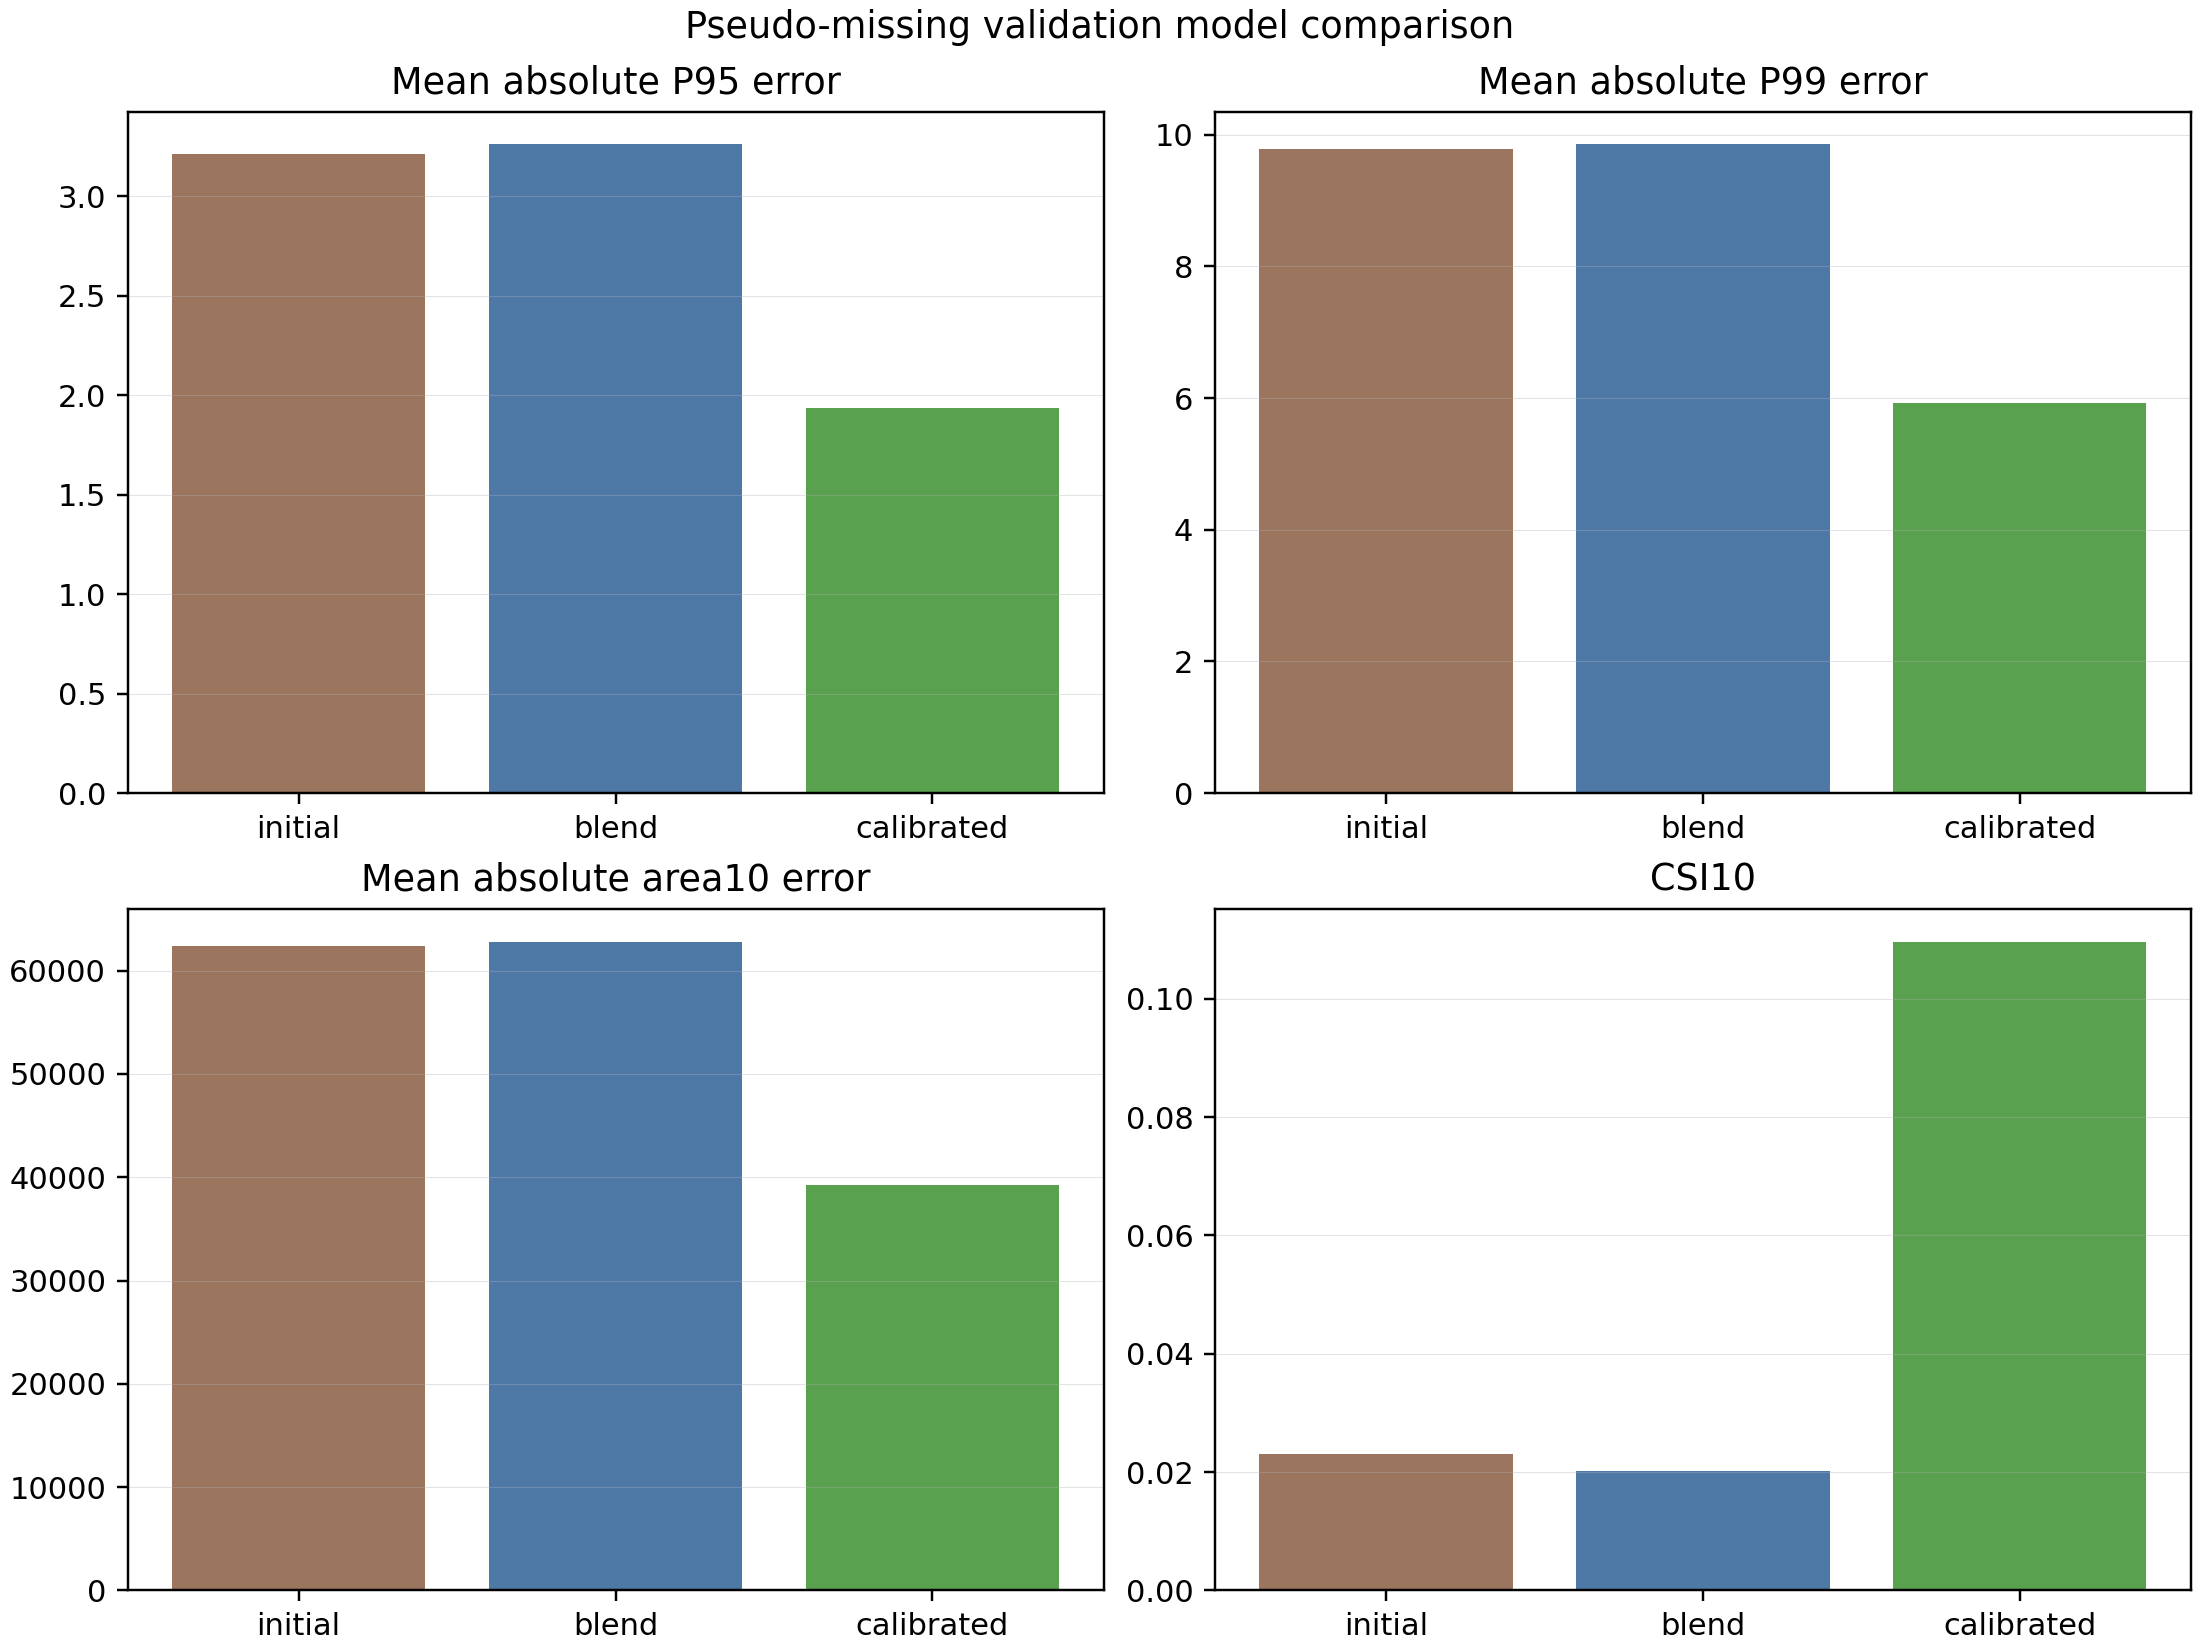
\includegraphics[width=0.85\textwidth]{outputs/figures/problem2_final_results/problem2_final_validation_model_comparison.png}
\caption{伪缺失验证中不同模型版本的极端降水评价指标对比}
\label{fig:p2_validation_comparison}
\end{figure}

\subsubsection{关键参数敏感性分析}

前文模型中包含若干经验性超参数，包括 Top-$K$ 相似样本数量、相似距离各分量权重以及 EOF/PCA 融合系数 $\beta$。为检验参数设置对生成结果的影响，本文基于历史台风伪缺失验证框架进一步开展关键参数敏感性分析。为保证不同设置之间可比，选取与伪缺失验证一致的 $8$ 个历史验证事件，每个事件抽取 $60$ 个半小时时次，共 $480$ 个有效验证时次。每组参数均重新执行相似检索、模板迁移、EOF/PCA 融合和极端分位数校准，并统计 calibrated 版本与真实 GPM 降水场之间的误差。

敏感性分析的参数设置如表 \ref{tab:p2_sensitivity_setting} 所示。其中基准设置为 $K=20$、强度权重 $1.5$、移动权重 $1.2$、环境权重 $1.2$、EOF/PCA 融合系数 $\beta=0.3$。S1 与 S2 分别用于检验相似样本数量减少和增加时的影响；S3--S5 用于检验主要距离权重扰动；S6 与 S7 用于检验 EOF/PCA 融合强度变化。

\begin{table}[H]
\centering
\caption{相似检索与结构融合参数敏感性设置}
\label{tab:p2_sensitivity_setting}
\resizebox{\textwidth}{!}{
\begin{tabular}{lcccccc}
\toprule
设置 & $K$ & 强度权重 & 移动权重 & 环境权重 & EOF融合系数$\beta$ & 目的 \\
\midrule
基准 & 20 & 1.5 & 1.2 & 1.2 & 0.3 & 当前模型设定 \\
S1 & 10 & 1.5 & 1.2 & 1.2 & 0.3 & 检验较少相似样本时的稳定性 \\
S2 & 30 & 1.5 & 1.2 & 1.2 & 0.3 & 检验更多相似样本是否引入噪声 \\
S3 & 20 & 1.2 & 1.2 & 1.2 & 0.3 & 检验强度权重下降的影响 \\
S4 & 20 & 1.5 & 1.5 & 1.2 & 0.3 & 检验移动特征权重上升的影响 \\
S5 & 20 & 1.5 & 1.2 & 1.5 & 0.3 & 检验海陆环境权重上升的影响 \\
S6 & 20 & 1.5 & 1.2 & 1.2 & 0.0 & 不使用 EOF/PCA 融合 \\
S7 & 20 & 1.5 & 1.2 & 1.2 & 0.5 & 提高 EOF/PCA 融合强度 \\
\bottomrule
\end{tabular}}
\end{table}

各参数设置下的主要验证指标如表 \ref{tab:p2_sensitivity_result} 所示。总体来看，不同参数设置下 P95 误差、P99 误差、强降水面积误差和 CSI10 均未出现突变，说明本文生成模型对关键超参数具有一定鲁棒性。

\begin{table}[H]
\centering
\caption{关键参数敏感性分析结果}
\label{tab:p2_sensitivity_result}
\resizebox{\textwidth}{!}{
\begin{tabular}{lccccccccc}
\toprule
设置 & RMSE & MAE & Corr & P95误差 & P99误差 & Rmax误差 & $A_{10}$误差 & CSI10 & F1\_10 \\
\midrule
基准 & 2.7355 & 0.9749 & 0.3614 & 1.9761 & 6.1577 & 19.7977 & 40352.9 & 0.1160 & 0.1867 \\
S1 & 2.8055 & 0.9977 & 0.3371 & 2.0271 & 5.7534 & 15.5196 & 40074.8 & 0.1108 & 0.1791 \\
S2 & 2.7219 & 0.9706 & 0.3658 & 1.9990 & 6.3977 & 21.6752 & 40733.1 & 0.1153 & 0.1857 \\
S3 & 2.7313 & 0.9746 & 0.3606 & 1.9817 & 6.1744 & 19.8931 & 40318.8 & 0.1157 & 0.1861 \\
S4 & 2.7328 & 0.9739 & 0.3630 & 1.9779 & 6.1738 & 19.7450 & 40338.3 & 0.1161 & 0.1866 \\
S5 & 2.7334 & 0.9744 & 0.3614 & 1.9887 & 6.1668 & 19.7821 & 40237.7 & 0.1153 & 0.1858 \\
S6 & 2.7620 & 0.9881 & 0.3492 & 1.9588 & 6.0119 & 17.8568 & 40232.9 & 0.1133 & 0.1830 \\
S7 & 2.7276 & 0.9687 & 0.3677 & 1.9967 & 6.2303 & 21.2688 & 40552.9 & 0.1176 & 0.1888 \\
\bottomrule
\end{tabular}}
\end{table}

由表 \ref{tab:p2_sensitivity_result} 可见，当 $K$ 从 $20$ 调整为 $10$ 或 $30$ 时，模型性能整体保持稳定。$K=10$ 时，P99 误差和 Rmax 误差有所下降，但 Corr 和 CSI10 略低于基准，说明较少相似样本可能更容易突出局地极端值，但也更容易受个别历史样本影响，空间结构稳定性略弱。$K=30$ 时，Corr 略有提高，但 P99 和 Rmax 误差增大，说明引入更多相似性较弱的历史样本可能平滑或扰动极端结构。因此，本文取 $K=20$，在历史模板多样性和样本相似性之间取得折中。

当强度权重由 $1.5$ 降至 $1.2$ 时，P95、P99 与 Rmax 误差均较基准略有增大或基本持平，说明强度变量对极端降水刻画具有必要作用，这与问题一中强度变量对 $R_{95}$、$R_{99}$ 和强降水面积影响稳定的结论一致。提高移动权重至 $1.5$ 后，Corr 略有提升，P95 误差基本不变，说明移动速度和移动方向主要影响雨带空间结构，而非单独决定极端强度。提高环境权重至 $1.5$ 后，强降水面积误差略有下降，但 CSI10 略降，说明近岸和海陆环境变量对强降水范围具有一定调制作用，但过高权重可能使样本匹配过度偏向地理环境相似性。

对 EOF/PCA 融合系数的敏感性结果显示，$\beta=0$ 时模型不使用 EOF/PCA 结构修正，P95、P99 与 Rmax 误差略低，但 Corr 和 CSI10 低于基准；$\beta=0.5$ 时 Corr、CSI10 和 F1\_10 略高，但 Rmax 误差有所增大。说明 EOF/PCA 融合可以提高大尺度结构稳定性和强降水识别能力，但过强的 EOF 约束可能进一步平滑局地极端峰值。综合极端误差、空间相关和强降水识别指标，$\beta=0.3$ 能在大尺度结构稳定性和局地极端保留之间取得较好平衡，因此作为本文最终设置。

综上，关键参数扰动下模型评价指标未发生方向性突变，表明本文相似检索--模板迁移--EOF/PCA 修正--极端校准的生成链条具有较好的参数鲁棒性。基准设置下虽然并非每一项指标均达到最优，但在 P95/P99 极端误差、强降水面积误差、CSI10 和空间相关性之间取得了较均衡的表现，适合作为后续 KONG-REY 与 MAN-YI 可能降水分布生成的最终参数组合。

\begin{figure}[H]
\centering
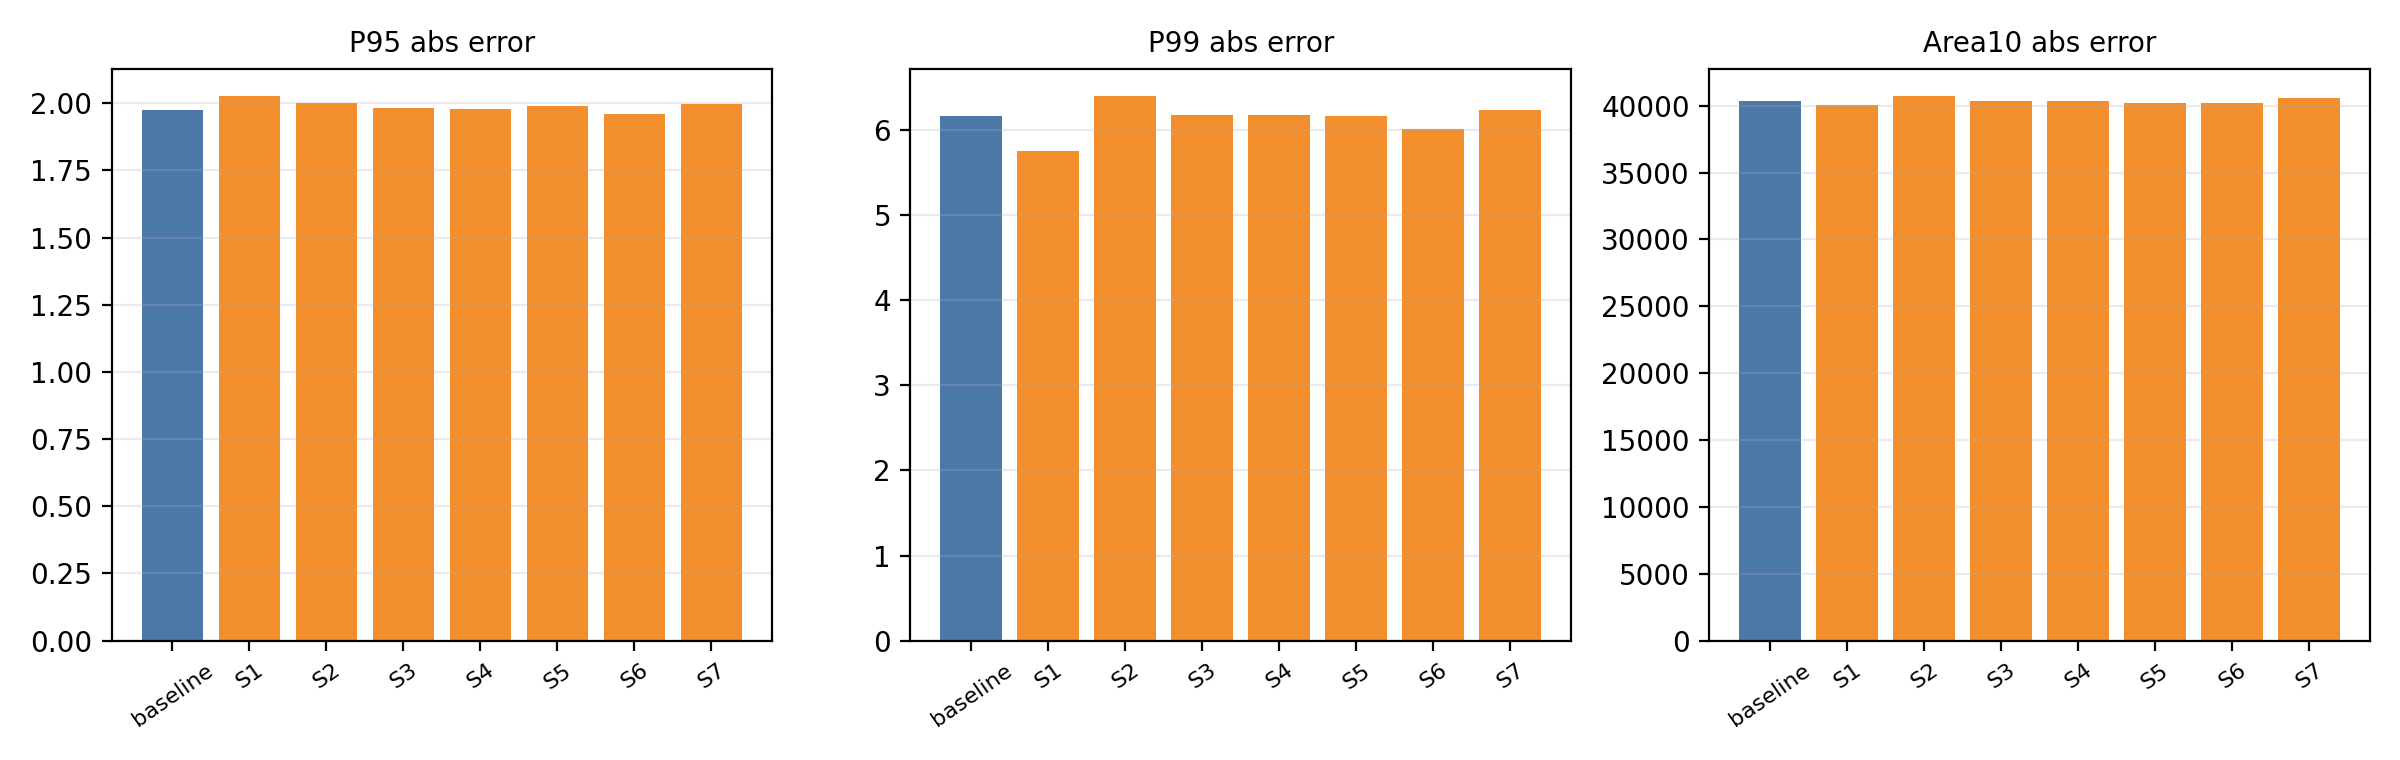
\includegraphics[width=0.9\textwidth]{outputs/figures/problem2_sensitivity_analysis/sensitivity_bar_extreme_errors.png}
\caption{不同参数设置下极端降水误差对比}
\label{fig:p2_sensitivity_extreme}
\end{figure}

\begin{figure}[H]
\centering
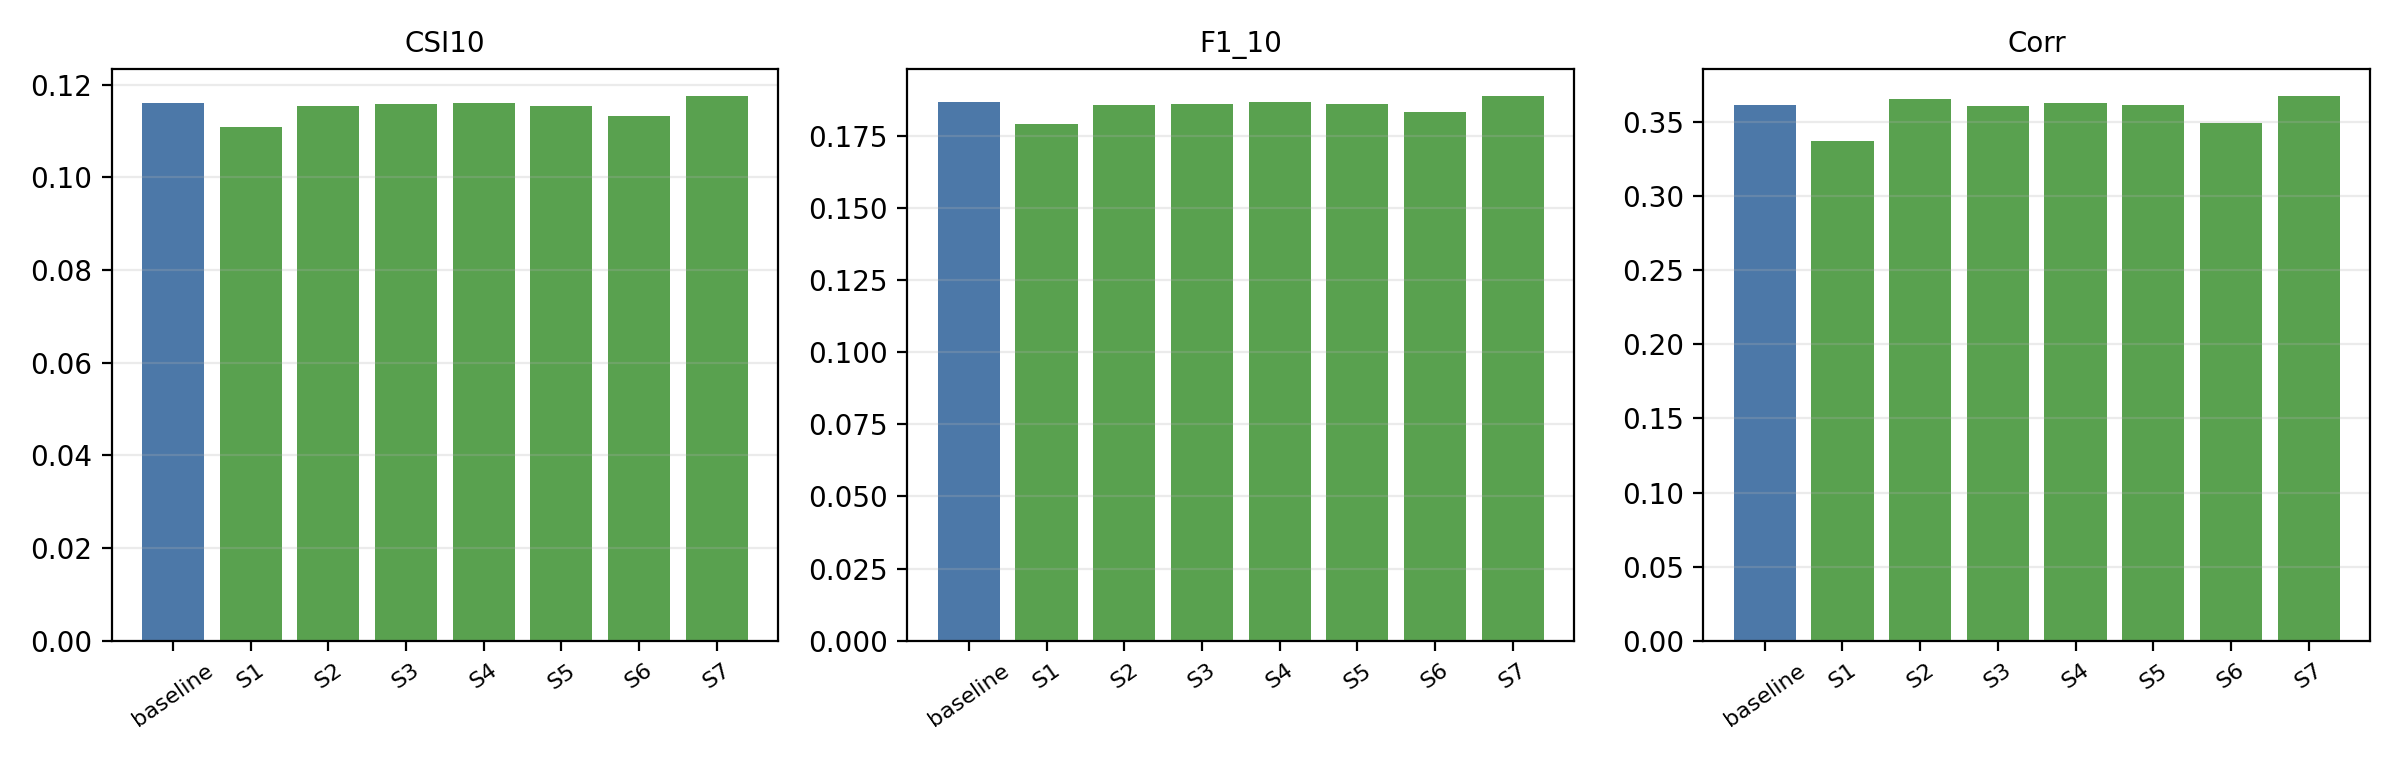
\includegraphics[width=0.9\textwidth]{outputs/figures/problem2_sensitivity_analysis/sensitivity_bar_skill_scores.png}
\caption{不同参数设置下空间相关与强降水识别指标对比}
\label{fig:p2_sensitivity_skill}
\end{figure}

\subsection{KONG-REY 与 MAN-YI 生成结果分析}

\subsubsection{最终结果说明}

基于 6.5 节得到的极端分位数校准场，本文得到 KONG-REY 和 MAN-YI 的最终半小时可能降水分布。需要强调的是，本结果为基于历史相似台风、路径强度条件和海陆环境生成的可能降水场，不是 GPM 真实观测。

表 \ref{tab:p2_final_summary_a} 和表 \ref{tab:p2_final_summary_b} 给出了两场台风的最终生成结果摘要。其中，表 \ref{tab:p2_final_summary_a} 侧重目标台风过程与 storm-relative 结构指标，表 \ref{tab:p2_final_summary_b} 侧重固定经纬度网格上的真实地理落区指标，从而区分降水结构随台风移动反复维持的持续性和真实地理位置经历强降水的累计时长。

\begingroup
\renewcommand{\thetable}{\thesection.\arabic{table}A}
\renewcommand{\theHtable}{\thetable}
\begin{table}[H]
\centering
\caption{目标台风过程与 storm-relative 结构指标}
\label{tab:p2_final_summary}
\label{tab:p2_final_summary_a}
\small
\setlength{\tabcolsep}{3pt}
\begin{tabular}{lcccccccc}
\toprule
台风 
& \makecell{过程\\时长/h}
& \makecell{WND最大值\\/(m/s)}
& \makecell{PRES最小值\\/hPa}
& \makecell{最大P95\\/(mm/h)}
& \makecell{最大P99\\/(mm/h)}
& \makecell{最大Rmax\\/(mm/h)}
& \makecell{最大$A_{10}$\\/km$^2$}
& \makecell{相对坐标\\$D_{10}^{\max}$/h} \\
\midrule
KONG-REY 
& 210.5 
& 60.0 
& 920.0 
& 3.8809 
& 16.8213 
& 53.7328 
& 87800.0 
& 146.0 \\
MAN-YI 
& 276.5 
& 62.0 
& 920.0 
& 4.9931 
& 17.1411 
& 54.4054 
& 115500.0 
& 196.0 \\
\bottomrule
\end{tabular}
\end{table}

\addtocounter{table}{-1}
\renewcommand{\thetable}{\thesection.\arabic{table}B}
\renewcommand{\theHtable}{\thetable}
\begin{table}[H]
\centering
\caption{真实地理坐标落区指标}
\label{tab:p2_final_summary_b}
\small
\setlength{\tabcolsep}{4pt}
\begin{tabularx}{\textwidth}{lcccc>{\raggedright\arraybackslash}X}
\toprule
台风
& \makecell{地理最大\\累计降水/mm}
& \makecell{地理\\$D_{10}^{\max}$/h}
& \makecell{$P_{\mathrm{geo}}\ge100$ mm\\面积/km$^2$}
& \makecell{$D_{10,\mathrm{geo}}\ge3$ h\\面积/km$^2$}
& 主要特征 \\
\midrule
KONG-REY
& 722.047
& 27.0
& $1.229\times 10^6$
& $8.055\times 10^5$
& \makecell[l]{局地累计峰值更高；\\固定地理单点持续时间略长} \\
MAN-YI
& 533.592
& 23.5
& $2.071\times 10^6$
& $1.307\times 10^6$
& \makecell[l]{累计雨区和持续强降水\\覆盖范围更广} \\
\bottomrule
\end{tabularx}
\end{table}
\endgroup

需要说明的是，表中“相对坐标$D_{10}^{\max}$”是在台风相对运动坐标系下统计得到的强降水持续结构指标，表示某一相对台风中心方位在台风生命史中反复处于强降水区的累计时长；“地理$D_{10}^{\max}$”则是在固定经纬度网格上统计得到的强降水持续时间，表示某一真实地理位置经历 $10\ \mathrm{mm/hr}$ 及以上强降水的累计时长。二者刻画对象不同，前者用于解释降水结构，后者用于刻画真实地理落区。

KONG-REY 的生成过程持续 $210.5$ h，最大风速为 $60.0$，最低气压为 $920.0$。其生成降水场中，最大格点雨强达到 $53.733\ \mathrm{mm/hr}$，发生于 2024-10-26 23:00:00；最大 P95 降水强度为 $3.881\ \mathrm{mm/hr}$，最大 P99 降水强度为 $16.821\ \mathrm{mm/hr}$，二者均发生于 2024-10-30 09:00:00；$10\ \mathrm{mm/hr}$ 以上强降水面积峰值为 $87800\ \mathrm{km^2}$，也发生于 2024-10-30 09:00:00。其累计降水体量代理值为 $4.930\times 10^8\ \mathrm{mm\cdot km^2}$。

MAN-YI 的生成过程持续 $276.5$ h，最大风速为 $62.0$，最低气压为 $920.0$。其最大格点雨强为 $54.405\ \mathrm{mm/hr}$，发生于 2024-11-14 10:30:00；最大 P95 为 $4.993\ \mathrm{mm/hr}$，发生于 2024-11-14 03:30:00；最大 P99 为 $17.141\ \mathrm{mm/hr}$，发生于 2024-11-14 04:30:00；$10\ \mathrm{mm/hr}$ 以上强降水面积峰值达到 $115500\ \mathrm{km^2}$，发生于 2024-11-14 04:00:00。其累计降水体量代理值为 $6.865\times 10^8\ \mathrm{mm\cdot km^2}$。

\subsubsection{两场台风对比}

从极端降水强度看，MAN-YI 的最大 P95、最大 P99 和最大格点雨强均略高于 KONG-REY；从空间范围看，MAN-YI 的 $10\ \mathrm{mm/hr}$ 强降水面积峰值为 $115500\ \mathrm{km^2}$，明显高于 KONG-REY 的 $87800\ \mathrm{km^2}$；从台风相对坐标下的结构持续性看，MAN-YI 的相对坐标 $D_{10}^{\max}$ 为 $196.0$ h，高于 KONG-REY 的 $146.0$ h，说明其强降水结构在相对台风中心方位上维持更久。固定经纬度落区上，KONG-REY 的地理 $D_{10}^{\max}$ 为 $27.0$ h，略高于 MAN-YI 的 $23.5$ h；但 MAN-YI 的 $P_{\mathrm{cum}}\ge100\ \mathrm{mm}$ 面积和 $D_{10}\ge3\ \mathrm{h}$ 面积均更大，表明其真实地理影响范围更广。

两场台风的累计降水主导象限均为移动方向左前侧（front\_left），说明生成结果保持了台风降水相对于移动方向的非对称结构特征。这与问题一中发现的台风降水质心偏移、移动方向和非对称雨带之间的关系一致。

\begin{figure}[H]
\centering
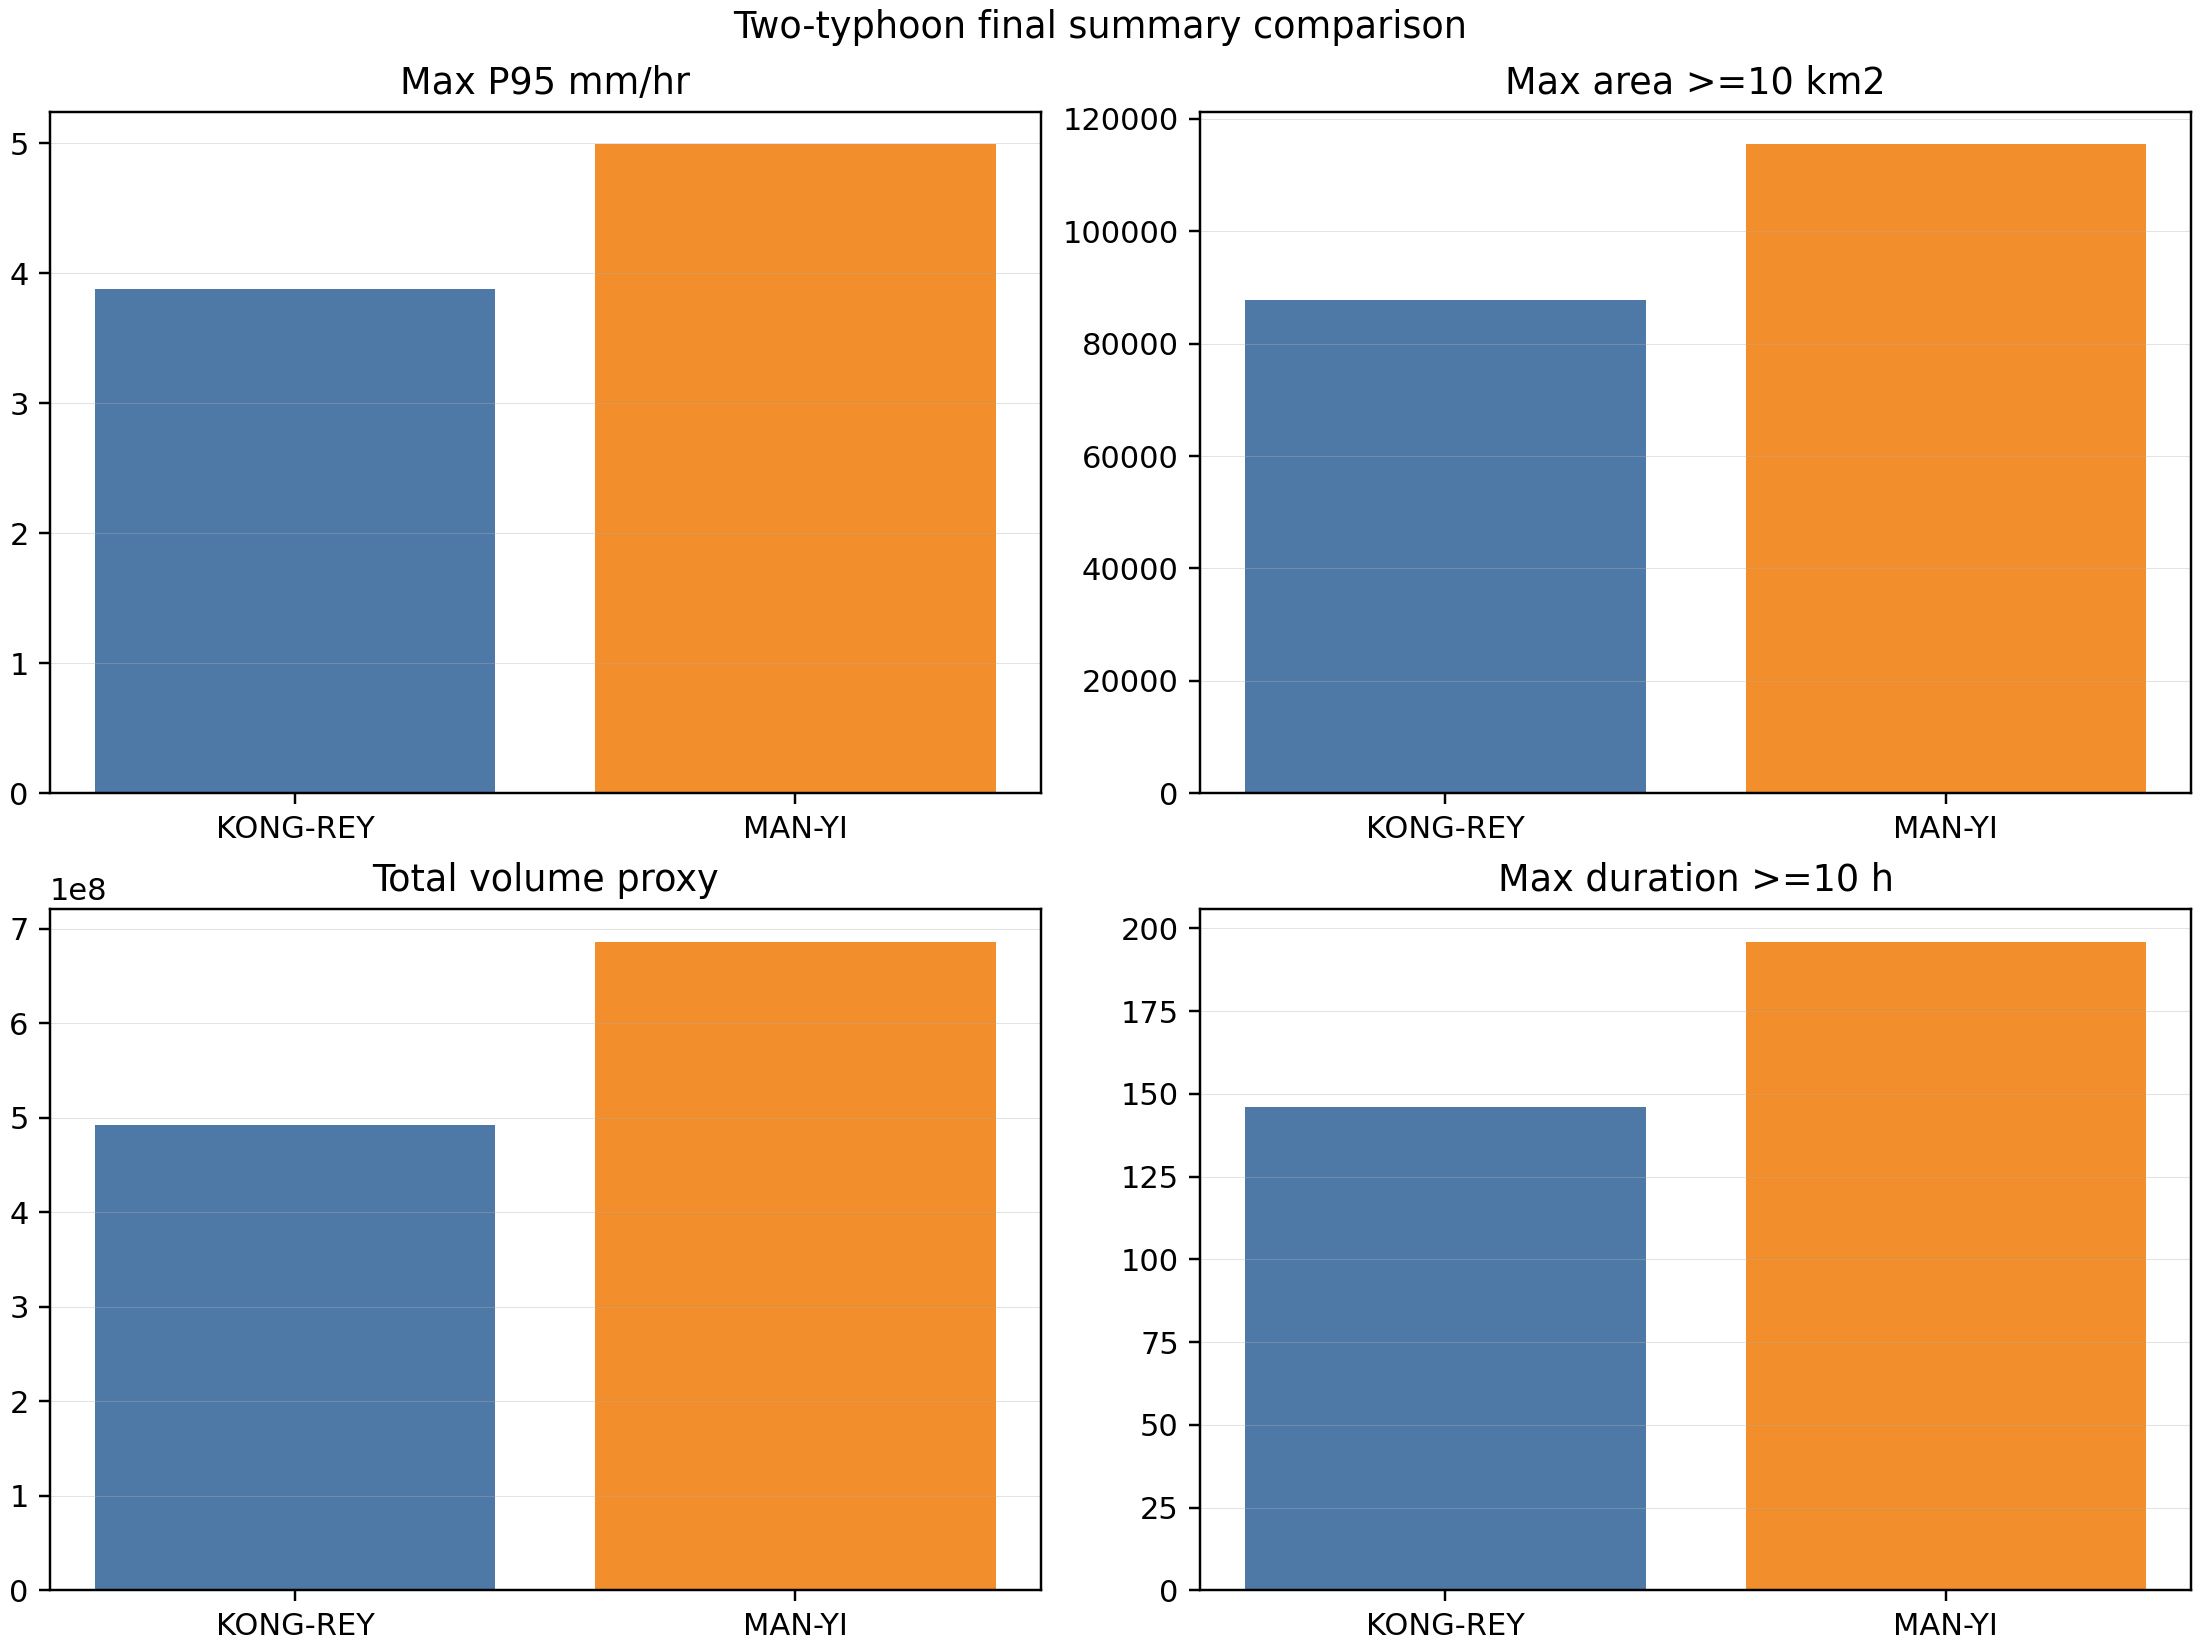
\includegraphics[width=0.95\textwidth]{outputs/figures/problem2_final_results/problem2_final_two_typhoons_summary_compare.png}
\caption{KONG-REY 与 MAN-YI 最终生成降水指标对比}
\label{fig:p2_two_typhoon_compare}
\end{figure}

\subsubsection{代表时刻降水场}

图 \ref{fig:p2_kongrey_fields} 和图 \ref{fig:p2_manyi_fields} 分别展示 KONG-REY 与 MAN-YI 的代表时刻台风相对坐标降水场。图中横轴为移动前方方向，纵轴为移动方向左侧。可以看出，两场台风在强度峰值和强降水面积峰值附近均形成较大范围的强降水区，且雨区相对于台风中心具有明显非对称性。

\begin{figure}[H]
\centering
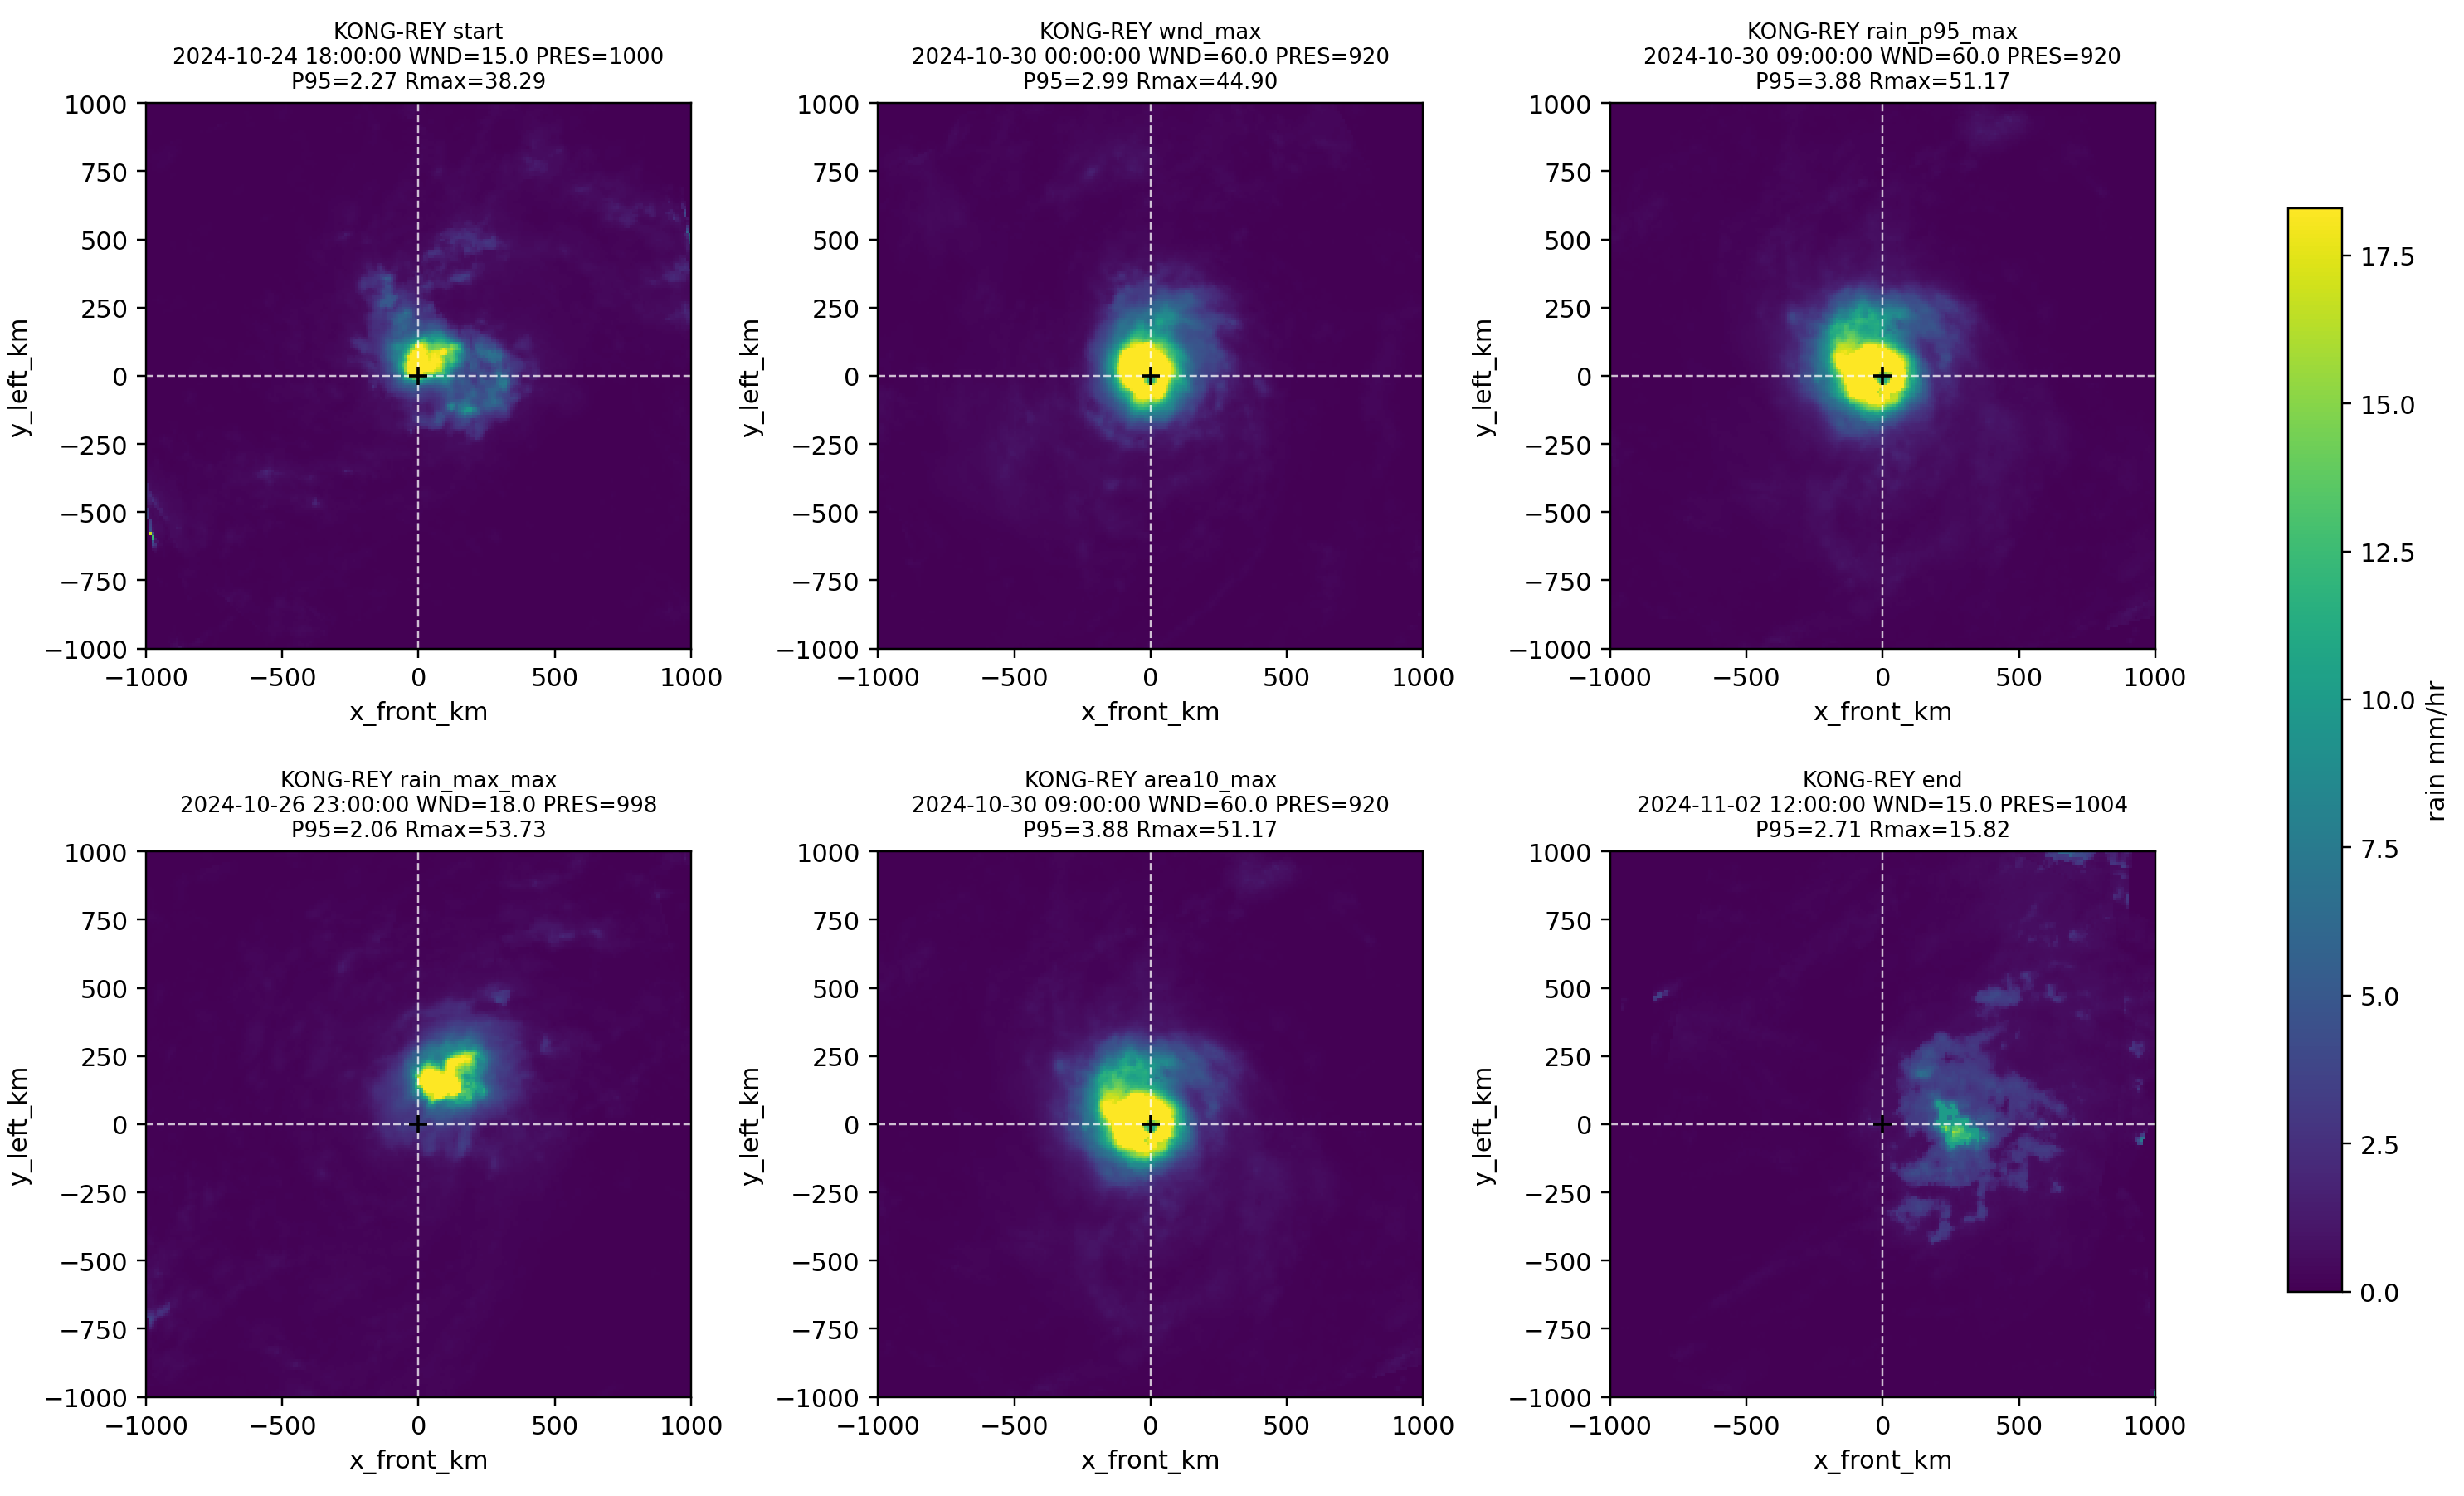
\includegraphics[width=0.95\textwidth]{outputs/figures/problem2_final_results/KONG_REY_final_representative_fields.png}
\caption{KONG-REY 代表时刻台风相对坐标降水场}
\label{fig:p2_kongrey_fields}
\end{figure}

\begin{figure}[H]
\centering
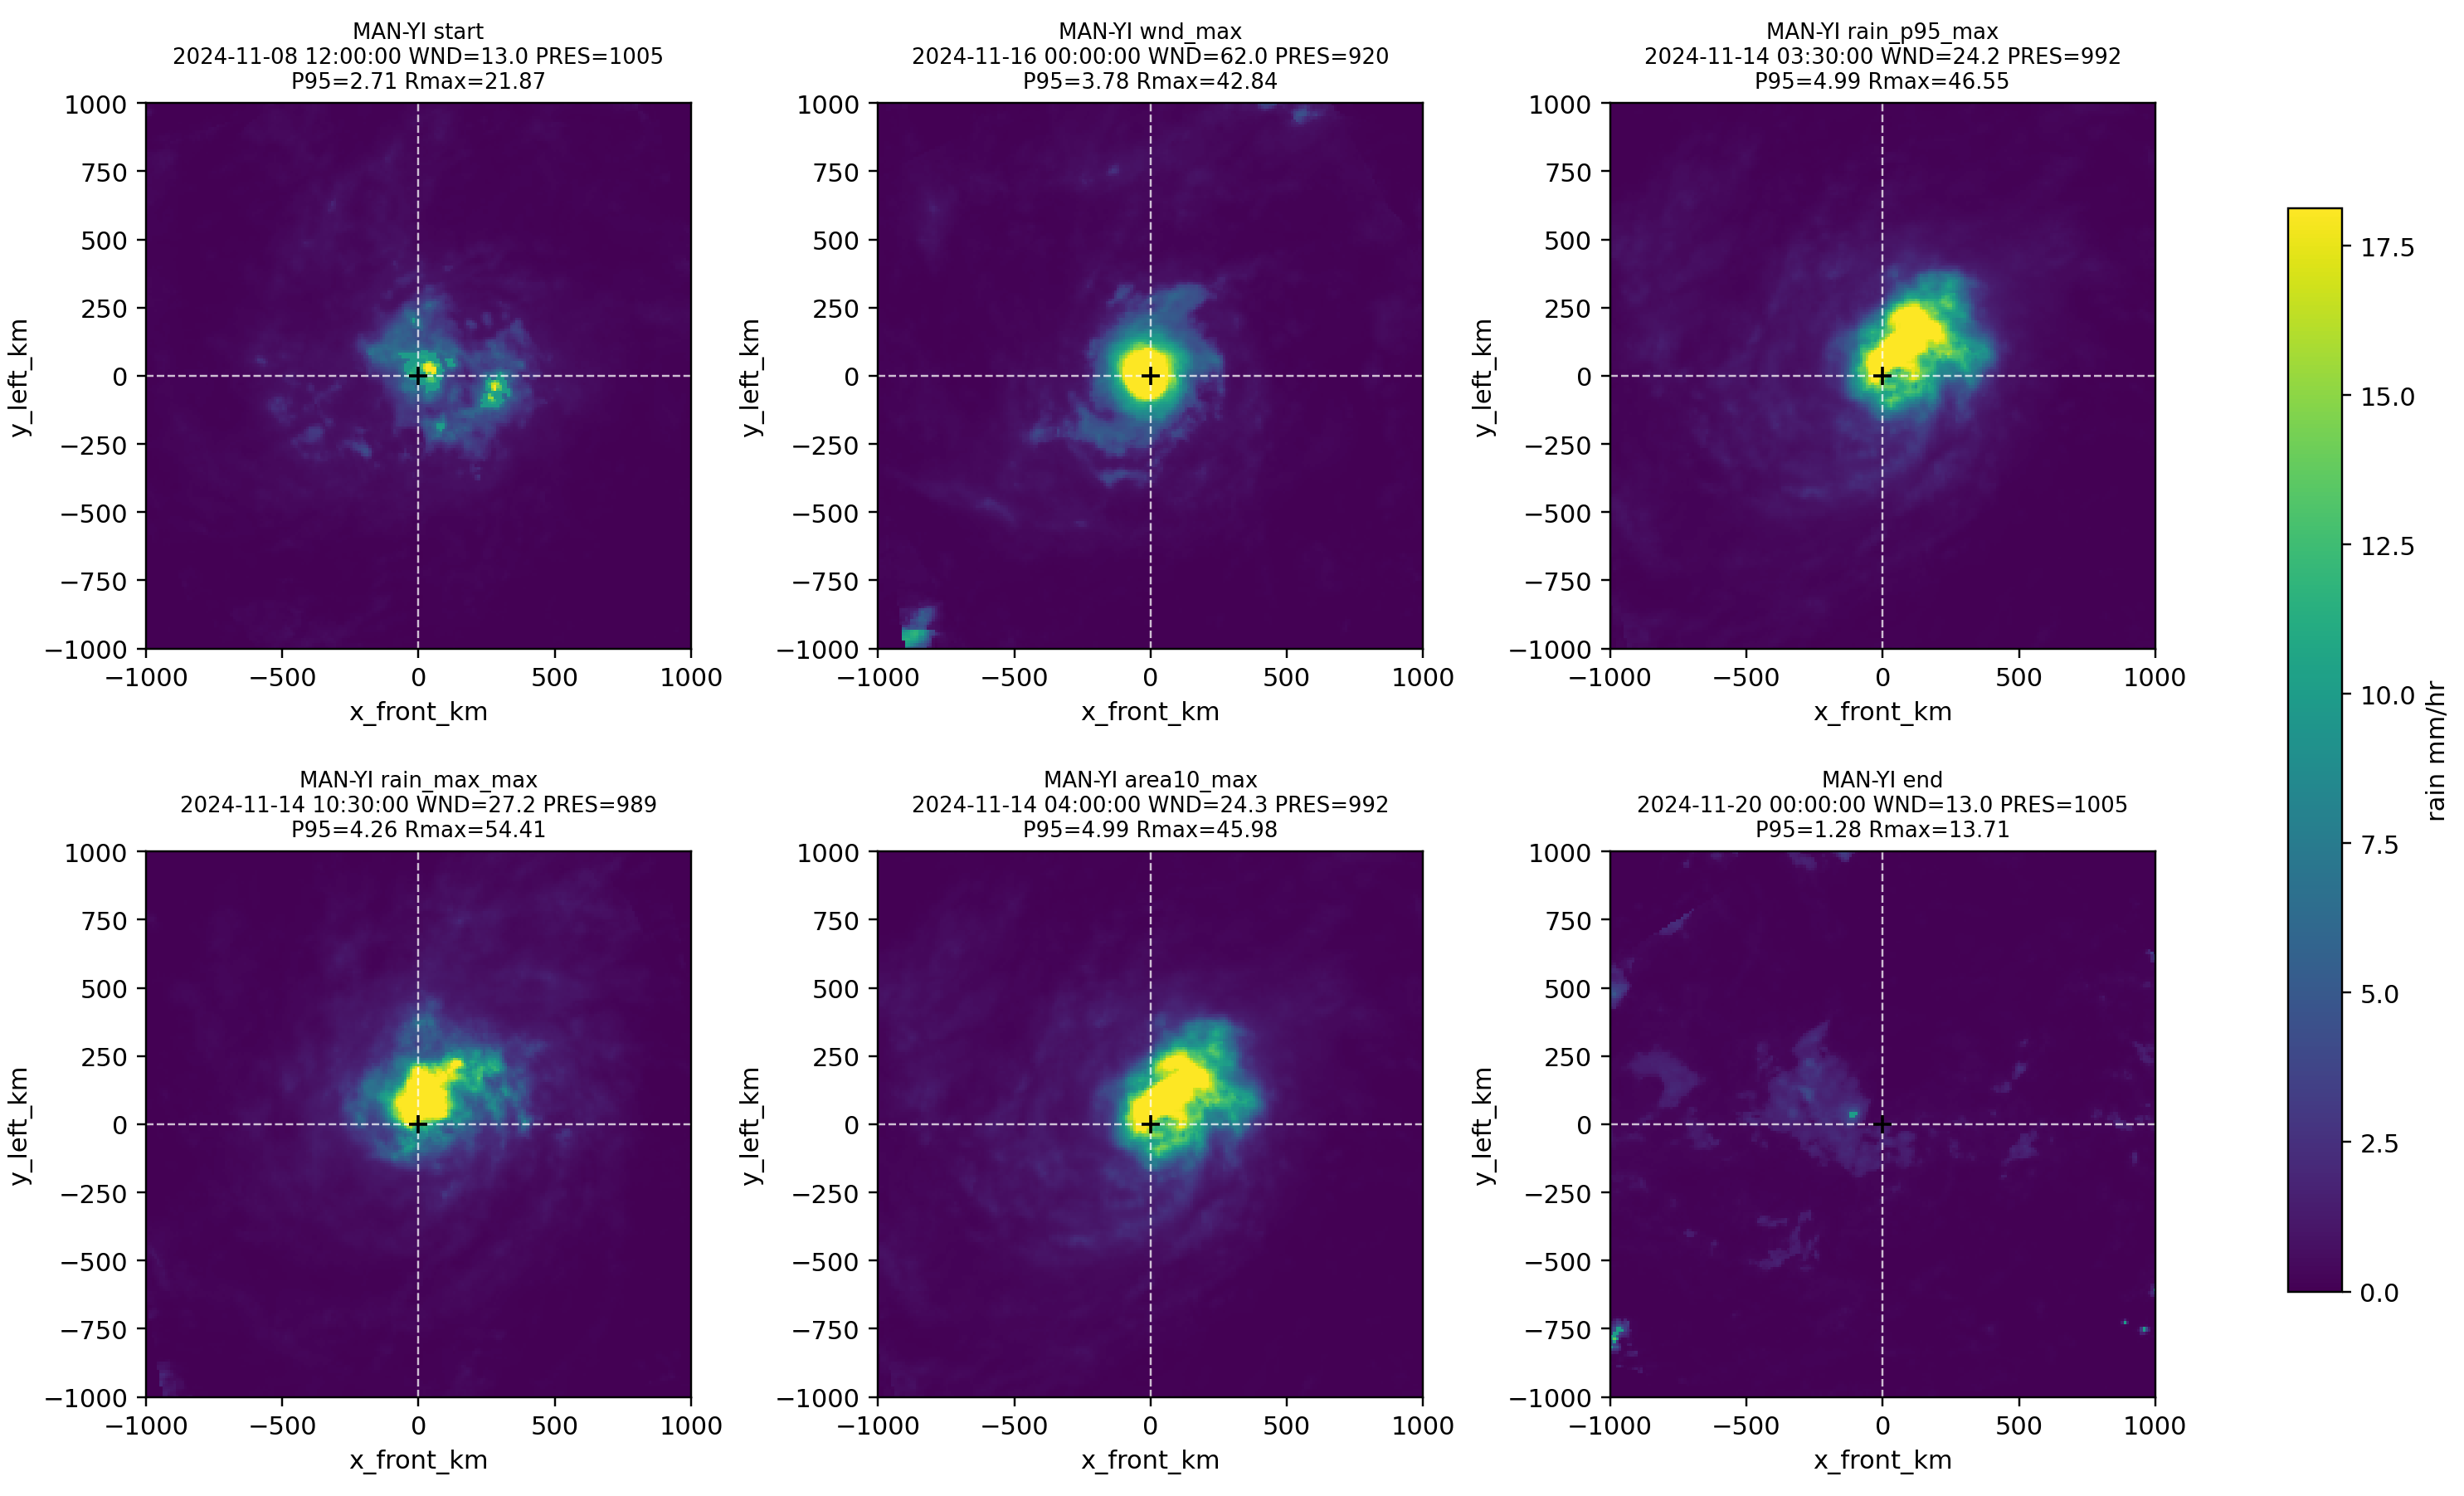
\includegraphics[width=0.95\textwidth]{outputs/figures/problem2_final_results/MAN_YI_final_representative_fields.png}
\caption{MAN-YI 代表时刻台风相对坐标降水场}
\label{fig:p2_manyi_fields}
\end{figure}

\subsubsection{累计降水、最大半小时降水与强降水持续时间}

本节给出的累计降水图、最大半小时降水图和强降水持续时间图均定位为 storm-relative 坐标下的结构解释图，而不是固定地理空间中的最终落区图。这些图是在台风相对运动坐标系下统计得到的，用于描述降水相对于台风中心及移动方向的结构特征，如主雨带位置、非对称性和持续性；它们不直接表示固定地理位置上的真实累计降水或持续时间。本文分别计算
\begin{equation}
P_{\mathrm{cum}}(x_f,y_l)
=
\sum_t 0.5R_t^{\mathrm{cal}}(x_f,y_l),
\end{equation}
\begin{equation}
R_{\max}^{\mathrm{grid}}(x_f,y_l)
=
\max_t R_t^{\mathrm{cal}}(x_f,y_l),
\end{equation}
\begin{equation}
D_{10}(x_f,y_l)
=
0.5\sum_t \mathbf{1}\left\{
R_t^{\mathrm{cal}}(x_f,y_l)\ge 10
\right\}.
\end{equation}
其中 $P_{\mathrm{cum}}$ 为半小时累计降水，$R_{\max}^{\mathrm{grid}}$ 为格点最大半小时降水强度，$D_{10}$ 为 $10\ \mathrm{mm/hr}$ 以上强降水持续时间指标。

\begin{figure}[H]
\centering
\begin{subfigure}{0.48\textwidth}
\centering
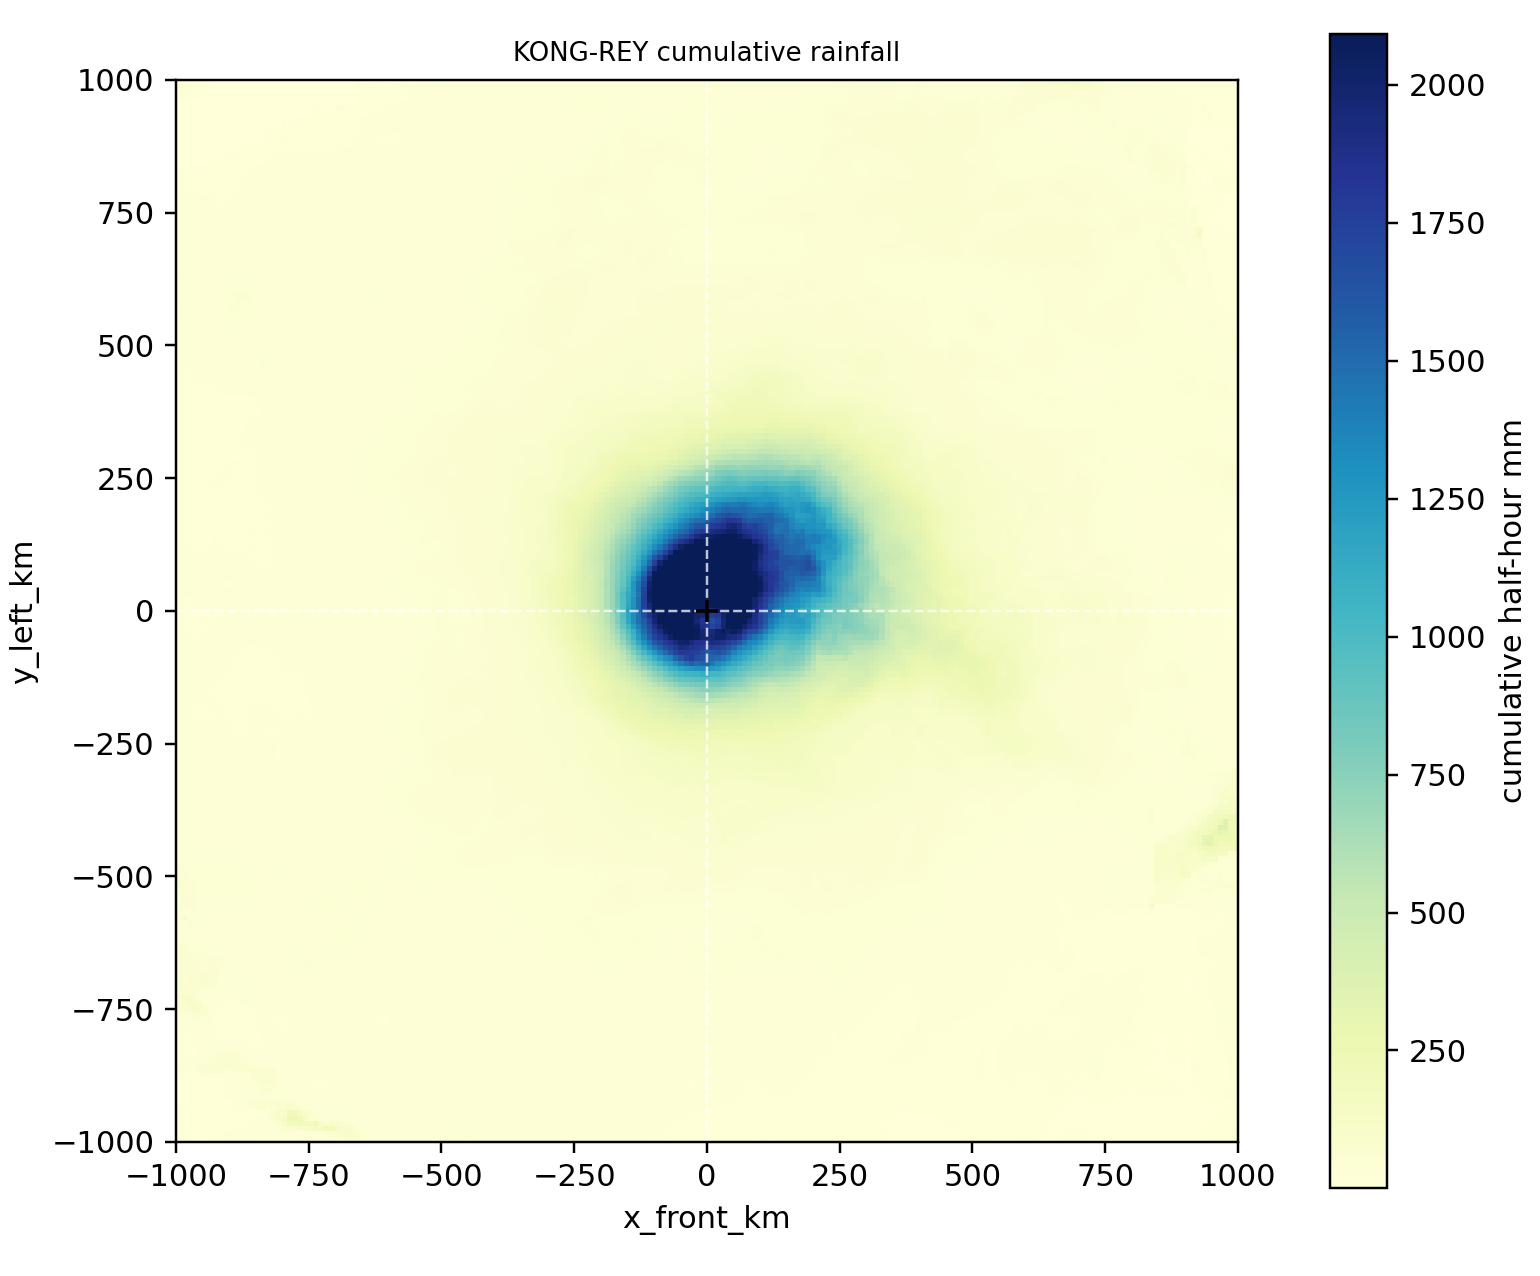
\includegraphics[width=\textwidth]{outputs/figures/problem2_final_results/KONG_REY_final_cumulative_rain_storm_relative.png}
\caption{KONG-REY storm-relative 累计降水结构}
\end{subfigure}
\begin{subfigure}{0.48\textwidth}
\centering
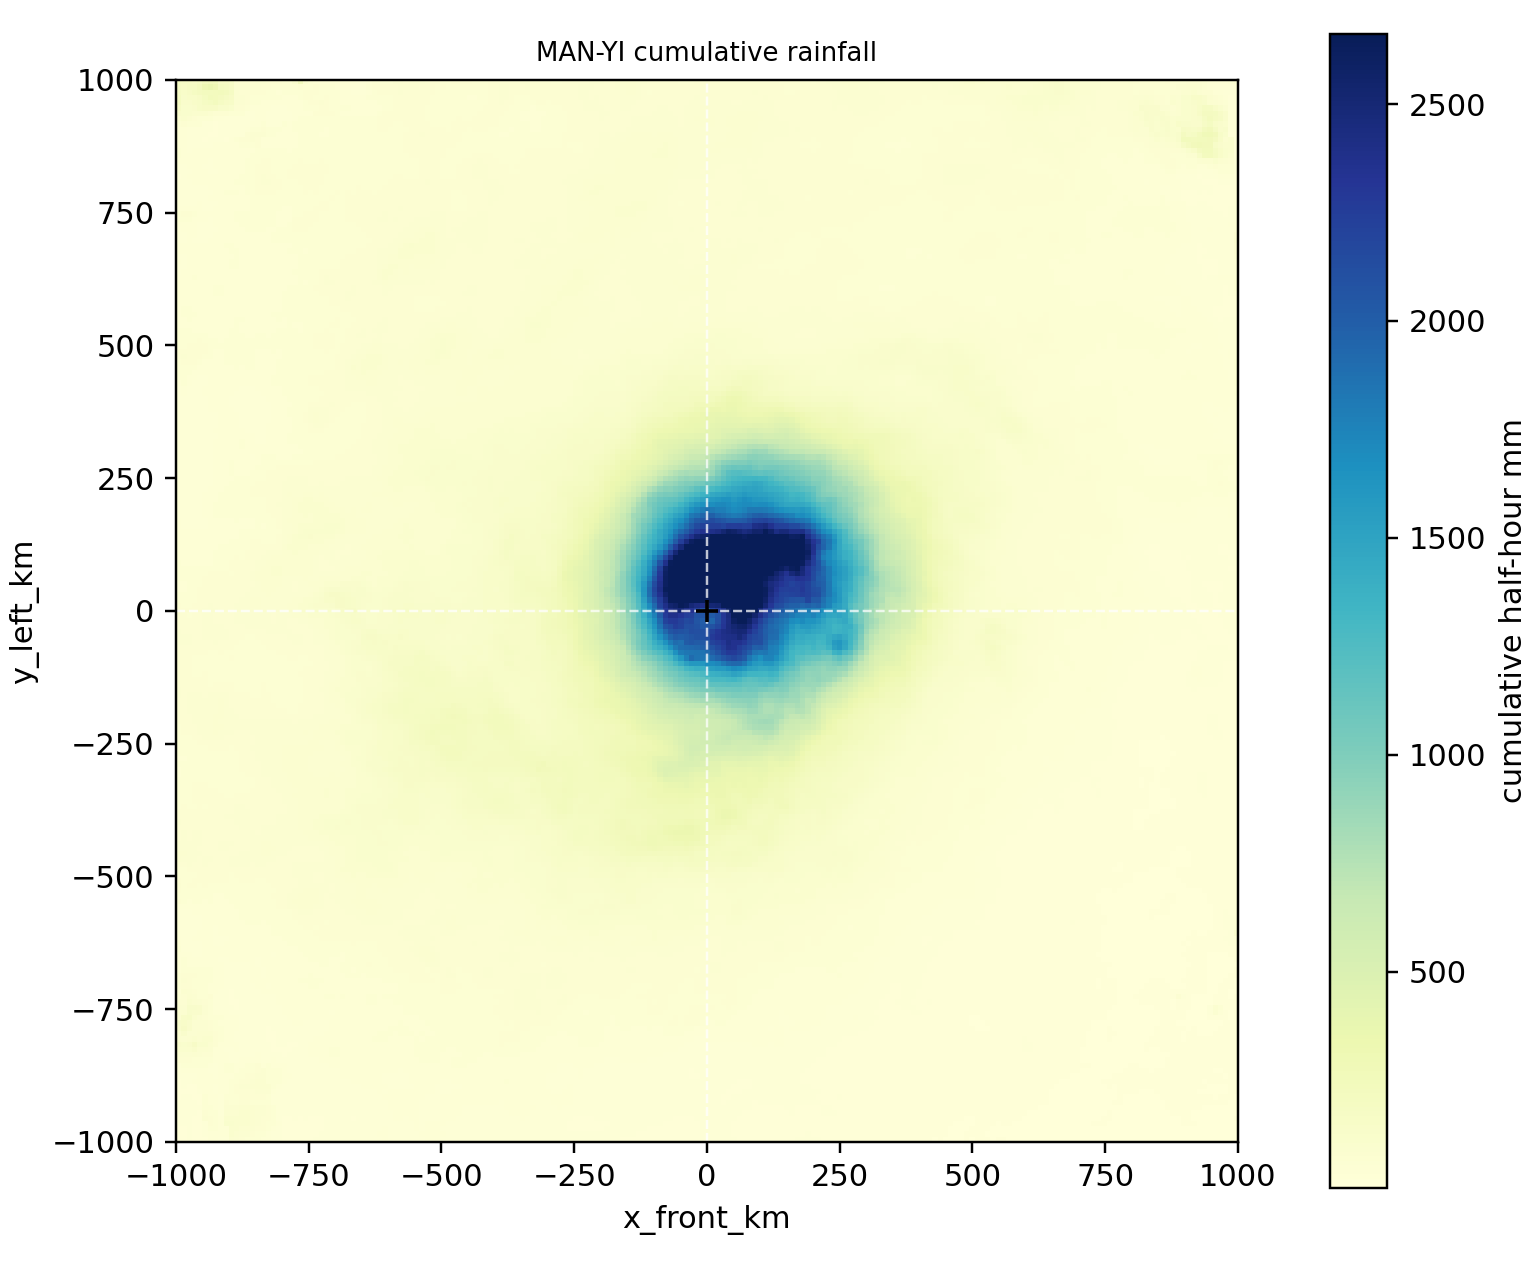
\includegraphics[width=\textwidth]{outputs/figures/problem2_final_results/MAN_YI_final_cumulative_rain_storm_relative.png}
\caption{MAN-YI storm-relative 累计降水结构}
\end{subfigure}
\caption{两场台风 storm-relative 累计降水结构解释图}
\label{fig:p2_cumulative_rain}
\end{figure}

\begin{figure}[H]
\centering
\begin{subfigure}{0.48\textwidth}
\centering
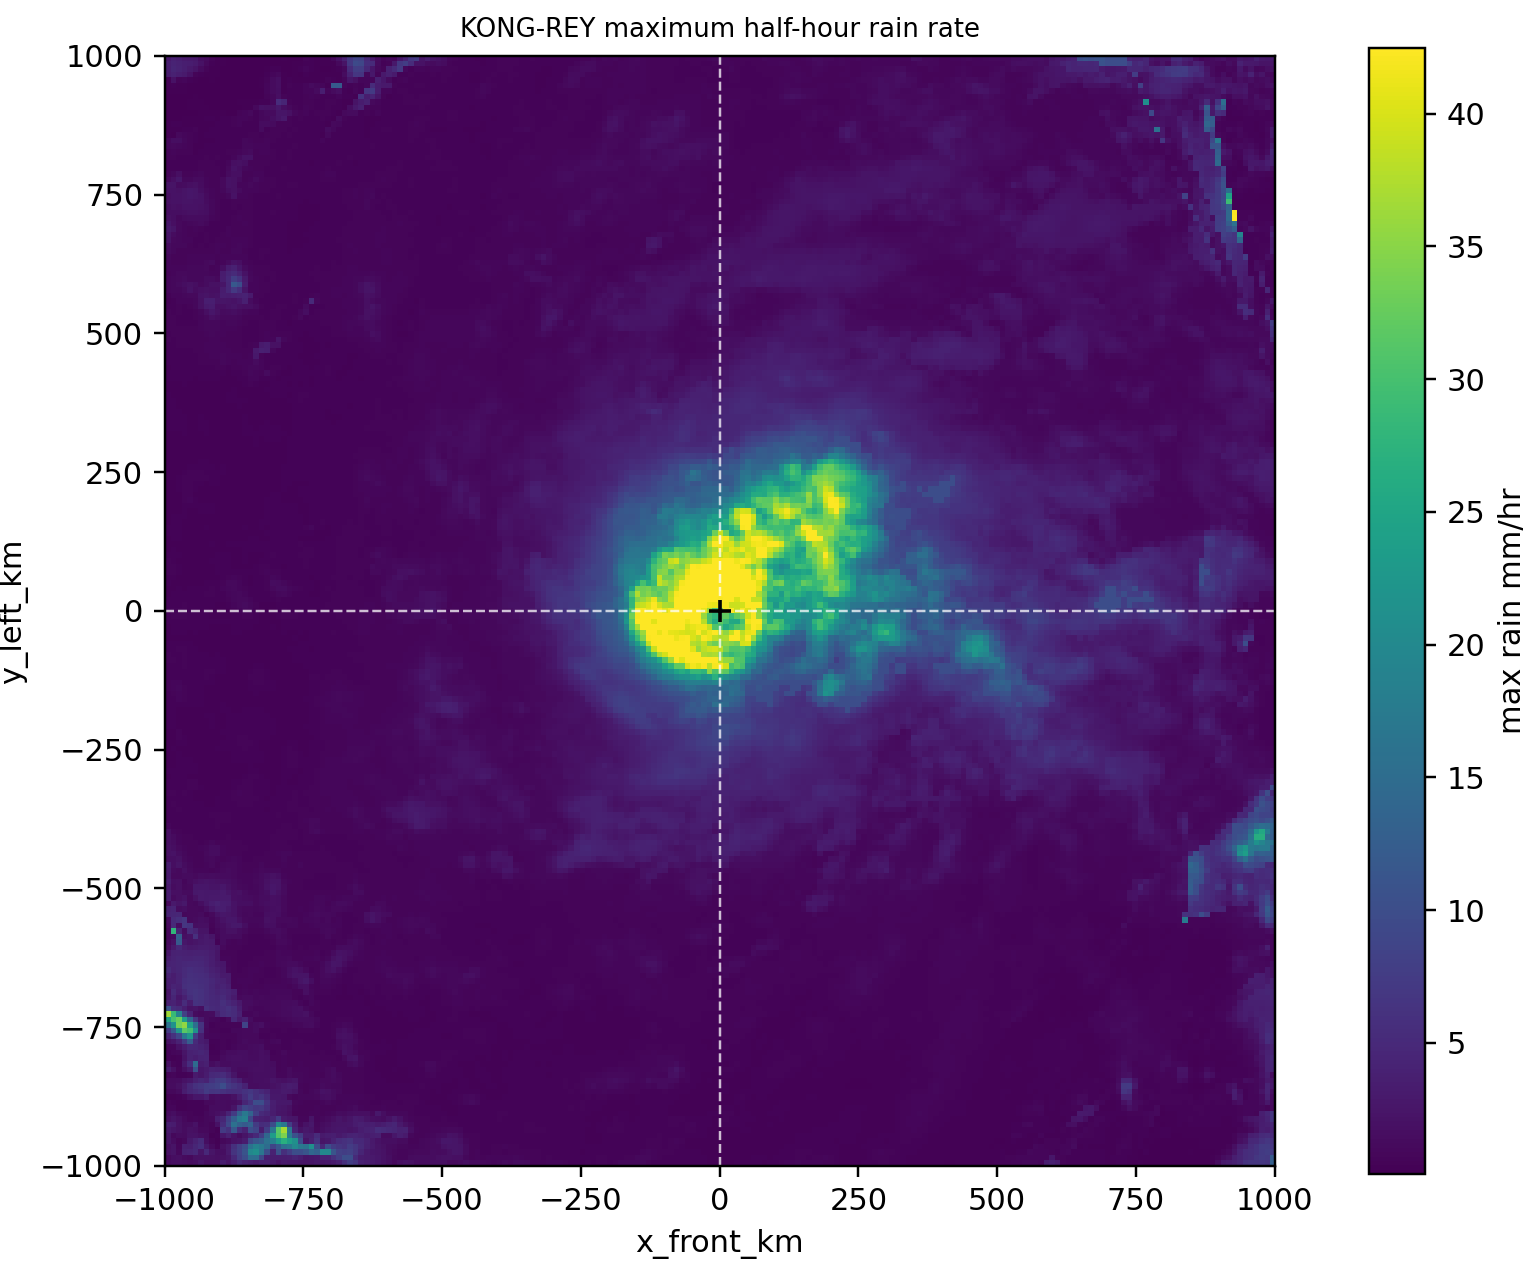
\includegraphics[width=\textwidth]{outputs/figures/problem2_final_results/KONG_REY_final_max_rain_storm_relative.png}
\caption{KONG-REY storm-relative 最大半小时降水结构}
\end{subfigure}
\begin{subfigure}{0.48\textwidth}
\centering
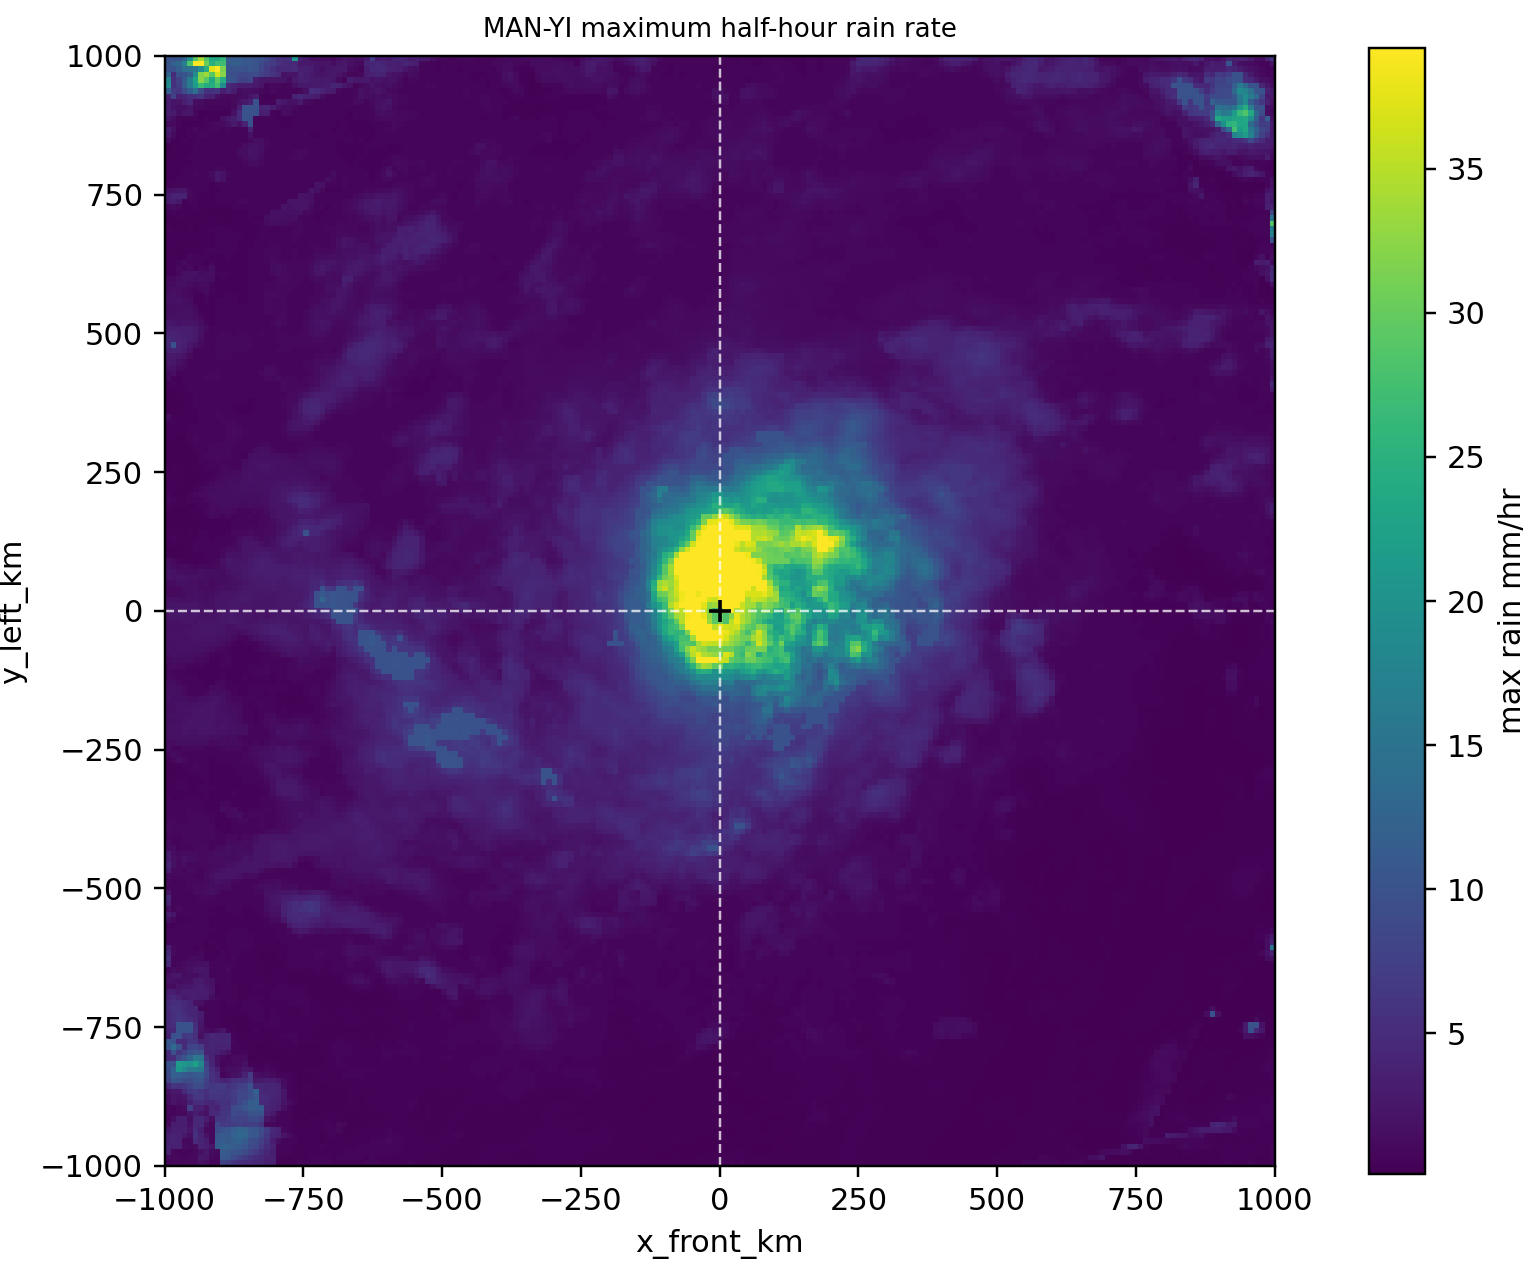
\includegraphics[width=\textwidth]{outputs/figures/problem2_final_results/MAN_YI_final_max_rain_storm_relative.png}
\caption{MAN-YI storm-relative 最大半小时降水结构}
\end{subfigure}
\caption{两场台风 storm-relative 最大半小时降水结构解释图}
\label{fig:p2_max_rain}
\end{figure}

\begin{figure}[H]
\centering
\begin{subfigure}{0.48\textwidth}
\centering
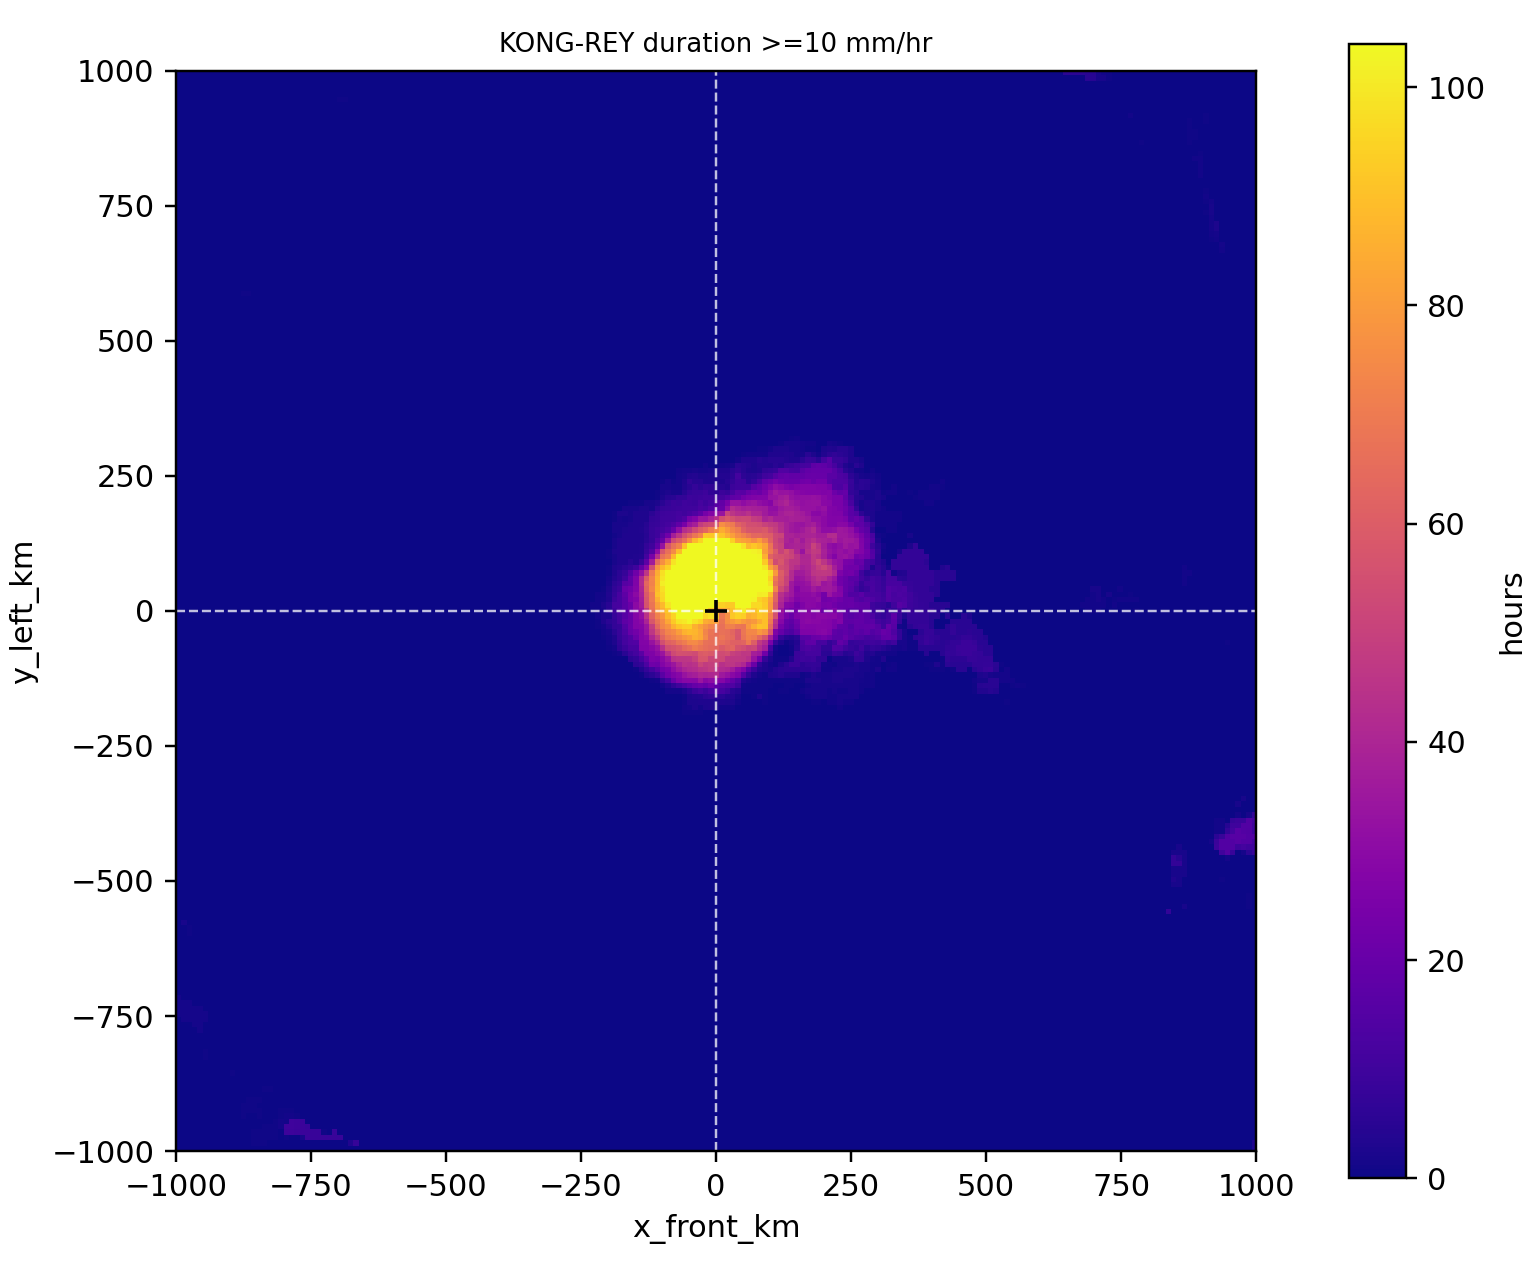
\includegraphics[width=\textwidth]{outputs/figures/problem2_final_results/KONG_REY_final_duration10_storm_relative.png}
\caption{KONG-REY storm-relative 强降水持续结构}
\end{subfigure}
\begin{subfigure}{0.48\textwidth}
\centering
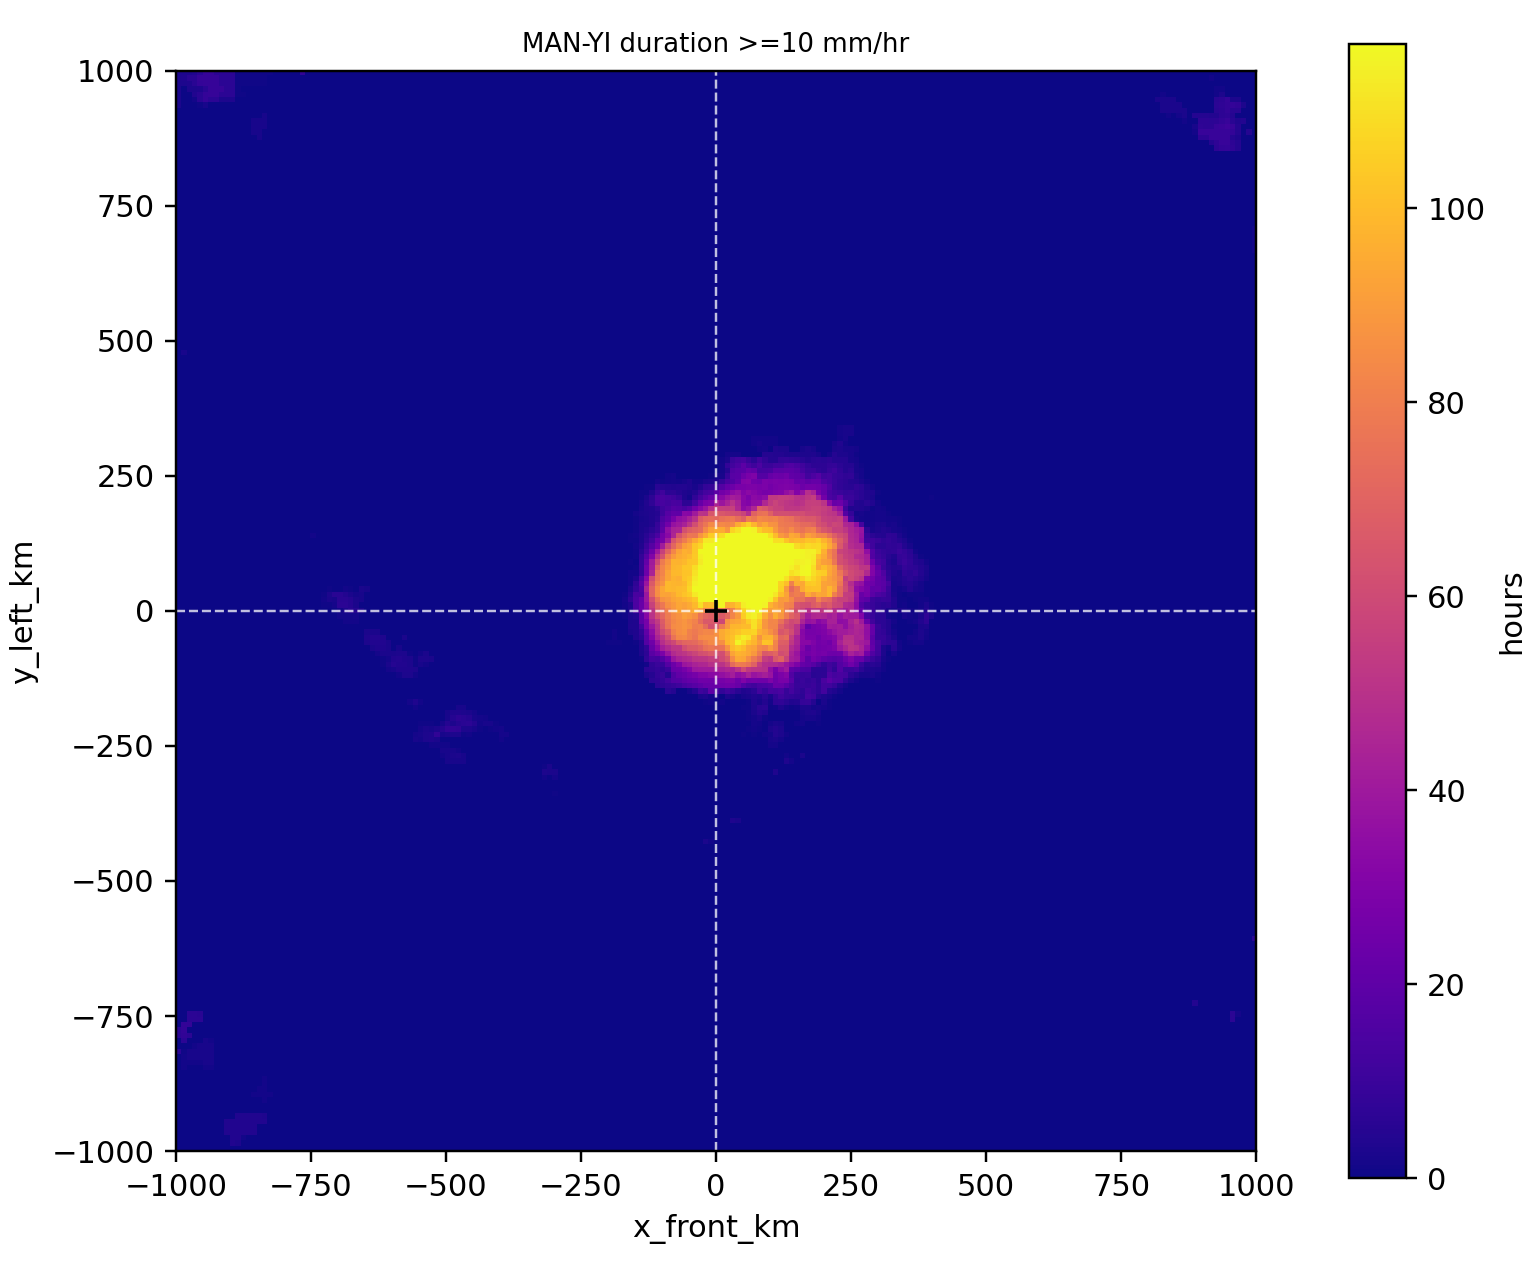
\includegraphics[width=\textwidth]{outputs/figures/problem2_final_results/MAN_YI_final_duration10_storm_relative.png}
\caption{MAN-YI storm-relative 强降水持续结构}
\end{subfigure}
\caption{$10\ \mathrm{mm/hr}$ 阈值下两场台风 storm-relative 强降水持续结构解释图}
\label{fig:p2_duration10}
\end{figure}

上述 storm-relative 图能够揭示台风降水结构相对于台风中心和移动方向的组织方式，但其坐标随台风中心移动而移动，并不对应固定地理位置上的降水累积。为进一步回答题目中“可能降水时空分布”的真实空间落区问题，下面将校准后的半小时降水场反投影到固定经纬度网格，计算地理累计降水和强降水持续时间。

\subsubsection{地理坐标下降水场反投影与真实落区分析}

前文给出的累计降水、最大半小时降水和强降水持续时间均是在台风相对运动坐标系下计算得到的，其主要作用是刻画降水相对于台风中心和移动方向的结构特征，例如主雨带所在象限、降水质心偏移、非对称性和雨带持续性等。该类结果有助于解释台风降水生成机理，但不能直接表示固定地理位置上的累计降水或强降水持续时间。

题目要求生成 KONG-REY 与 MAN-YI 的可能降水时空分布，因此仅给出 storm-relative 坐标下的结果是不充分的。为进一步得到真实经纬度意义下的降水落区，本文将极端分位数校准后的台风相对坐标降水场反投影到固定经纬度网格，计算地理累计降水、地理最大半小时降水和地理强降水持续时间。

设目标时刻 $t$ 的极端校准降水场为
\begin{equation}
R_t^{\mathrm{cal}}(x_f,y_l),
\end{equation}
其中 $x_f$ 表示沿台风移动方向前方的相对距离，$y_l$ 表示移动方向左侧的相对距离。记该时刻台风中心经纬度为 $(\lambda_{c,t},\phi_{c,t})$，移动方向角为 $\alpha_t$。根据台风相对运动坐标定义，可将相对坐标反变换到东西向和南北向距离：
\begin{equation}
x=x_f\sin\alpha_t-y_l\cos\alpha_t,
\qquad
y=x_f\cos\alpha_t+y_l\sin\alpha_t,
\end{equation}
其中 $x$ 表示东西向距离，$y$ 表示南北向距离，单位均为 km。

进一步将 $(x,y)$ 转换为经纬度坐标：
\begin{equation}
\lambda=\lambda_{c,t}
+\frac{x}{111.32\cos\phi_{c,t}},
\qquad
\phi=\phi_{c,t}
+\frac{y}{111.32}.
\end{equation}

实际计算时，为避免散点投影造成固定经纬度网格上的空洞，本文采用等价的反向采样方法。对固定地理网格上每个点 $(\lambda,\phi)$，先计算其相对于台风中心的东西向和南北向距离：
\begin{equation}
x=111.32\cos\phi_{c,t}(\lambda-\lambda_{c,t}),
\qquad
y=111.32(\phi-\phi_{c,t}),
\end{equation}
再转换为台风相对运动坐标：
\begin{equation}
x_f=x\sin\alpha_t+y\cos\alpha_t,
\qquad
y_l=-x\cos\alpha_t+y\sin\alpha_t.
\end{equation}
随后在 $R_t^{\mathrm{cal}}(x_f,y_l)$ 上进行双线性插值，得到固定经纬度网格上的半小时降水场
\begin{equation}
R_t^{\mathrm{geo}}(\lambda,\phi).
\end{equation}

在此基础上，定义真实地理坐标下的累计降水：
\begin{equation}
P_{\mathrm{geo}}(\lambda,\phi)
=
\sum_t 0.5 R_t^{\mathrm{geo}}(\lambda,\phi),
\end{equation}
其中 $0.5$ 为半小时累计因子，$P_{\mathrm{geo}}$ 的单位为 mm。

定义真实地理坐标下的最大半小时降水强度：
\begin{equation}
R_{\max,\mathrm{geo}}(\lambda,\phi)
=
\max_t R_t^{\mathrm{geo}}(\lambda,\phi).
\end{equation}

定义 $10\ \mathrm{mm/hr}$ 阈值下的地理强降水持续时间：
\begin{equation}
D_{10,\mathrm{geo}}(\lambda,\phi)
=
0.5\sum_t
\mathbf{1}
\left\{
R_t^{\mathrm{geo}}(\lambda,\phi)\ge 10
\right\},
\end{equation}
其中 $\mathbf{1}\{\cdot\}$ 为示性函数，$D_{10,\mathrm{geo}}$ 的单位为 h。该指标表示某一固定地理位置在整个台风过程中累计经历 $10\ \mathrm{mm/hr}$ 及以上强降水的总时长。

地理面积统计采用随纬度修正的经纬度网格面积。对于中心纬度为 $\phi$、分辨率为 $\Delta\lambda\times\Delta\phi$ 的网格单元，其面积近似为
\begin{equation}
A_{\mathrm{cell}}(\phi)
\approx
111.32^2\,\Delta\lambda\,\Delta\phi\,\cos\phi,
\end{equation}
单位为 km$^2$。因此，$P_{\mathrm{geo}}\ge100\ \mathrm{mm}$ 面积和 $D_{10,\mathrm{geo}}\ge3\ \mathrm{h}$ 面积均按满足阈值网格的 $A_{\mathrm{cell}}(\phi)$ 求和得到。

需要强调的是，$P_{\mathrm{geo}}(\lambda,\phi)$、$R_{\max,\mathrm{geo}}(\lambda,\phi)$ 和 $D_{10,\mathrm{geo}}(\lambda,\phi)$ 是用于回答真实地理空间落区的最终结果；而前文 storm-relative 坐标下的结果主要用于解释降水结构相对于台风中心和移动方向的组织形式。二者互为补充，不能相互替代。

本文以 $0.1^\circ$ 为经纬度网格分辨率，分别对 KONG-REY 与 MAN-YI 构建覆盖其路径及周边影响范围的固定地理网格。KONG-REY 的反投影网格范围为 $111.0^\circ\mathrm{E}$--$155.0^\circ\mathrm{E}$、$4.0^\circ\mathrm{N}$--$43.0^\circ\mathrm{N}$；MAN-YI 的反投影网格范围为 $103.0^\circ\mathrm{E}$--$172.0^\circ\mathrm{E}$、$2.0^\circ\mathrm{N}$--$27.0^\circ\mathrm{N}$。反投影后所有地理降水场均未出现 NaN、Inf、负值或全零异常。

图 \ref{fig:p2_geo_cum_rain} 给出了两场台风的真实地理累计降水分布。KONG-REY 的地理累计降水最大值为 $722.047\ \mathrm{mm}$，位于 $124.9^\circ\mathrm{E}$、$18.6^\circ\mathrm{N}$；MAN-YI 的地理累计降水最大值为 $533.592\ \mathrm{mm}$，位于 $153.2^\circ\mathrm{E}$、$13.9^\circ\mathrm{N}$。从局地累计峰值看，KONG-REY 更高。

\begin{figure}[H]
\centering
\begin{subfigure}{0.48\textwidth}
\centering
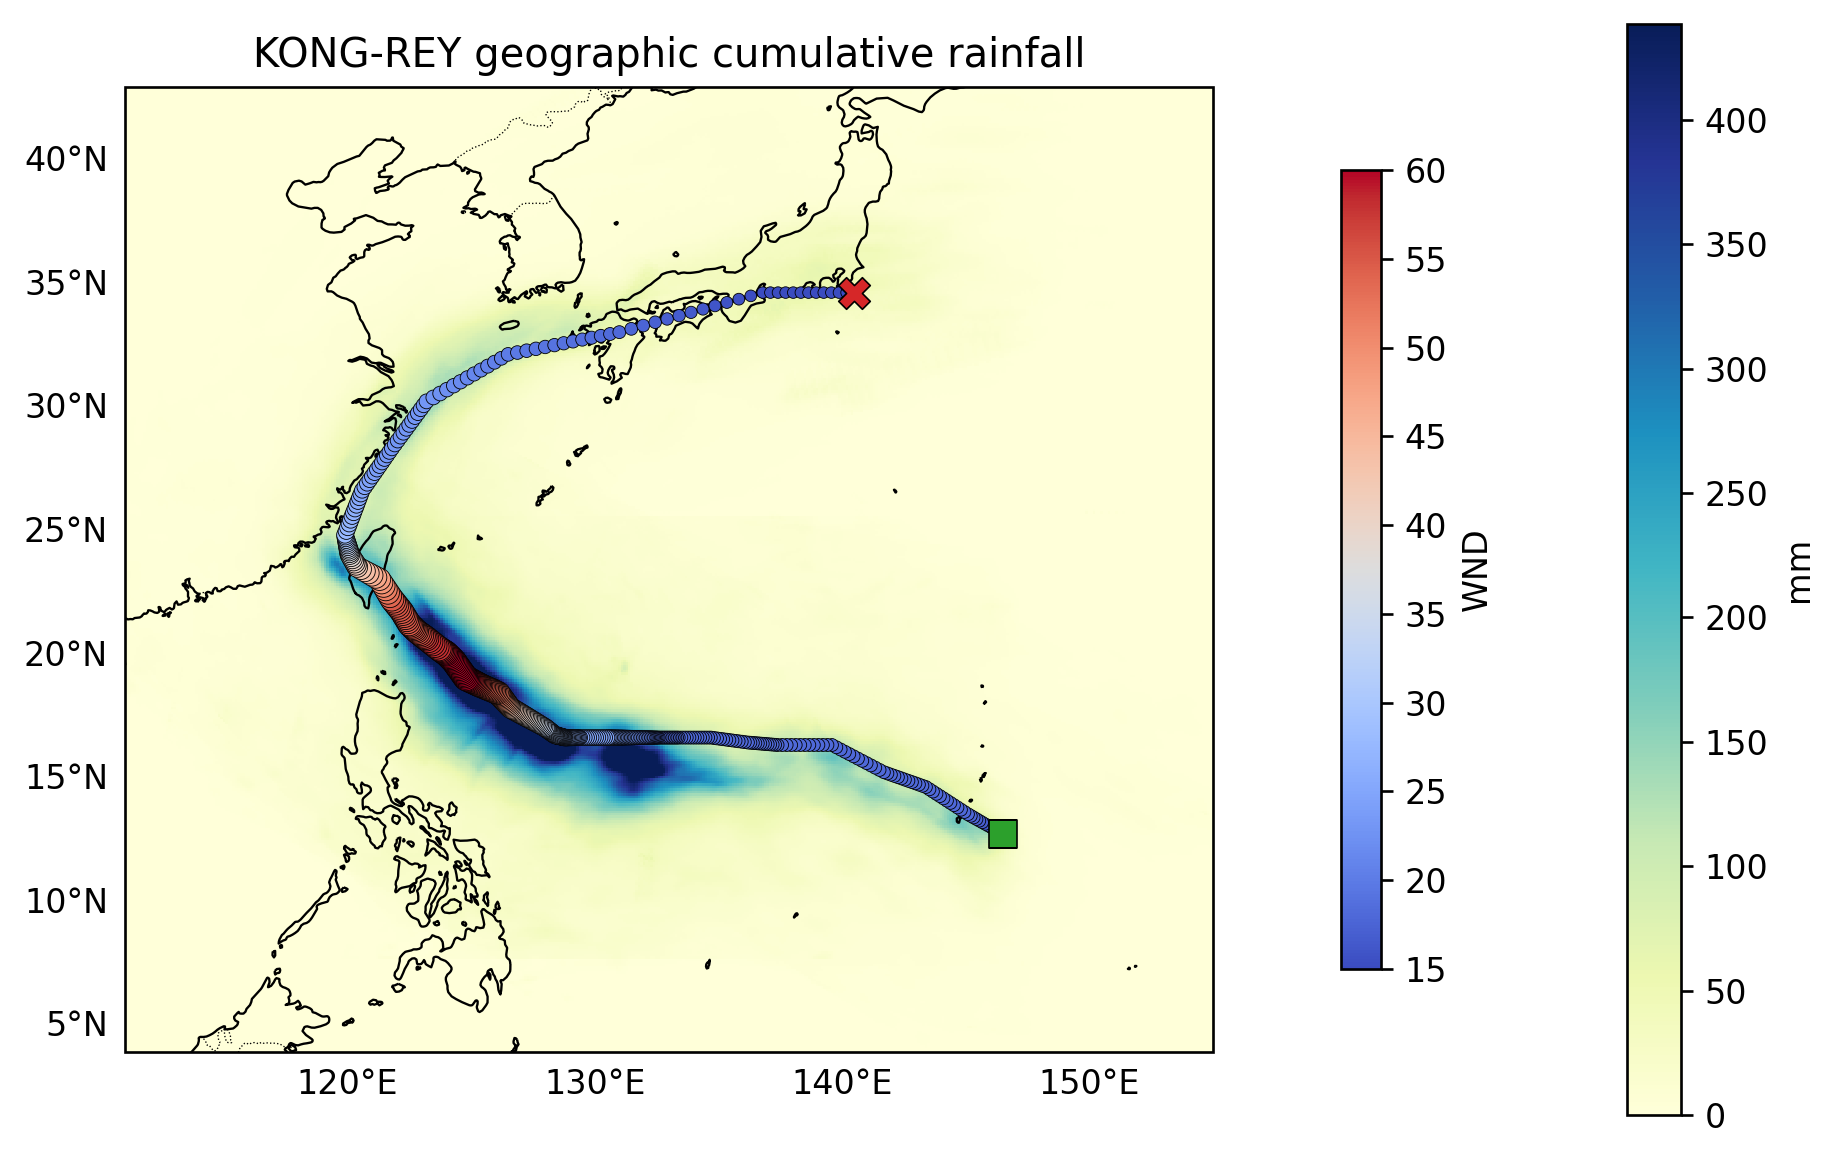
\includegraphics[width=\textwidth]{outputs/figures/problem2_geographic_results/KONG_REY_final_cumulative_rain_geographic.png}
\caption{KONG-REY 地理累计降水}
\end{subfigure}
\begin{subfigure}{0.48\textwidth}
\centering
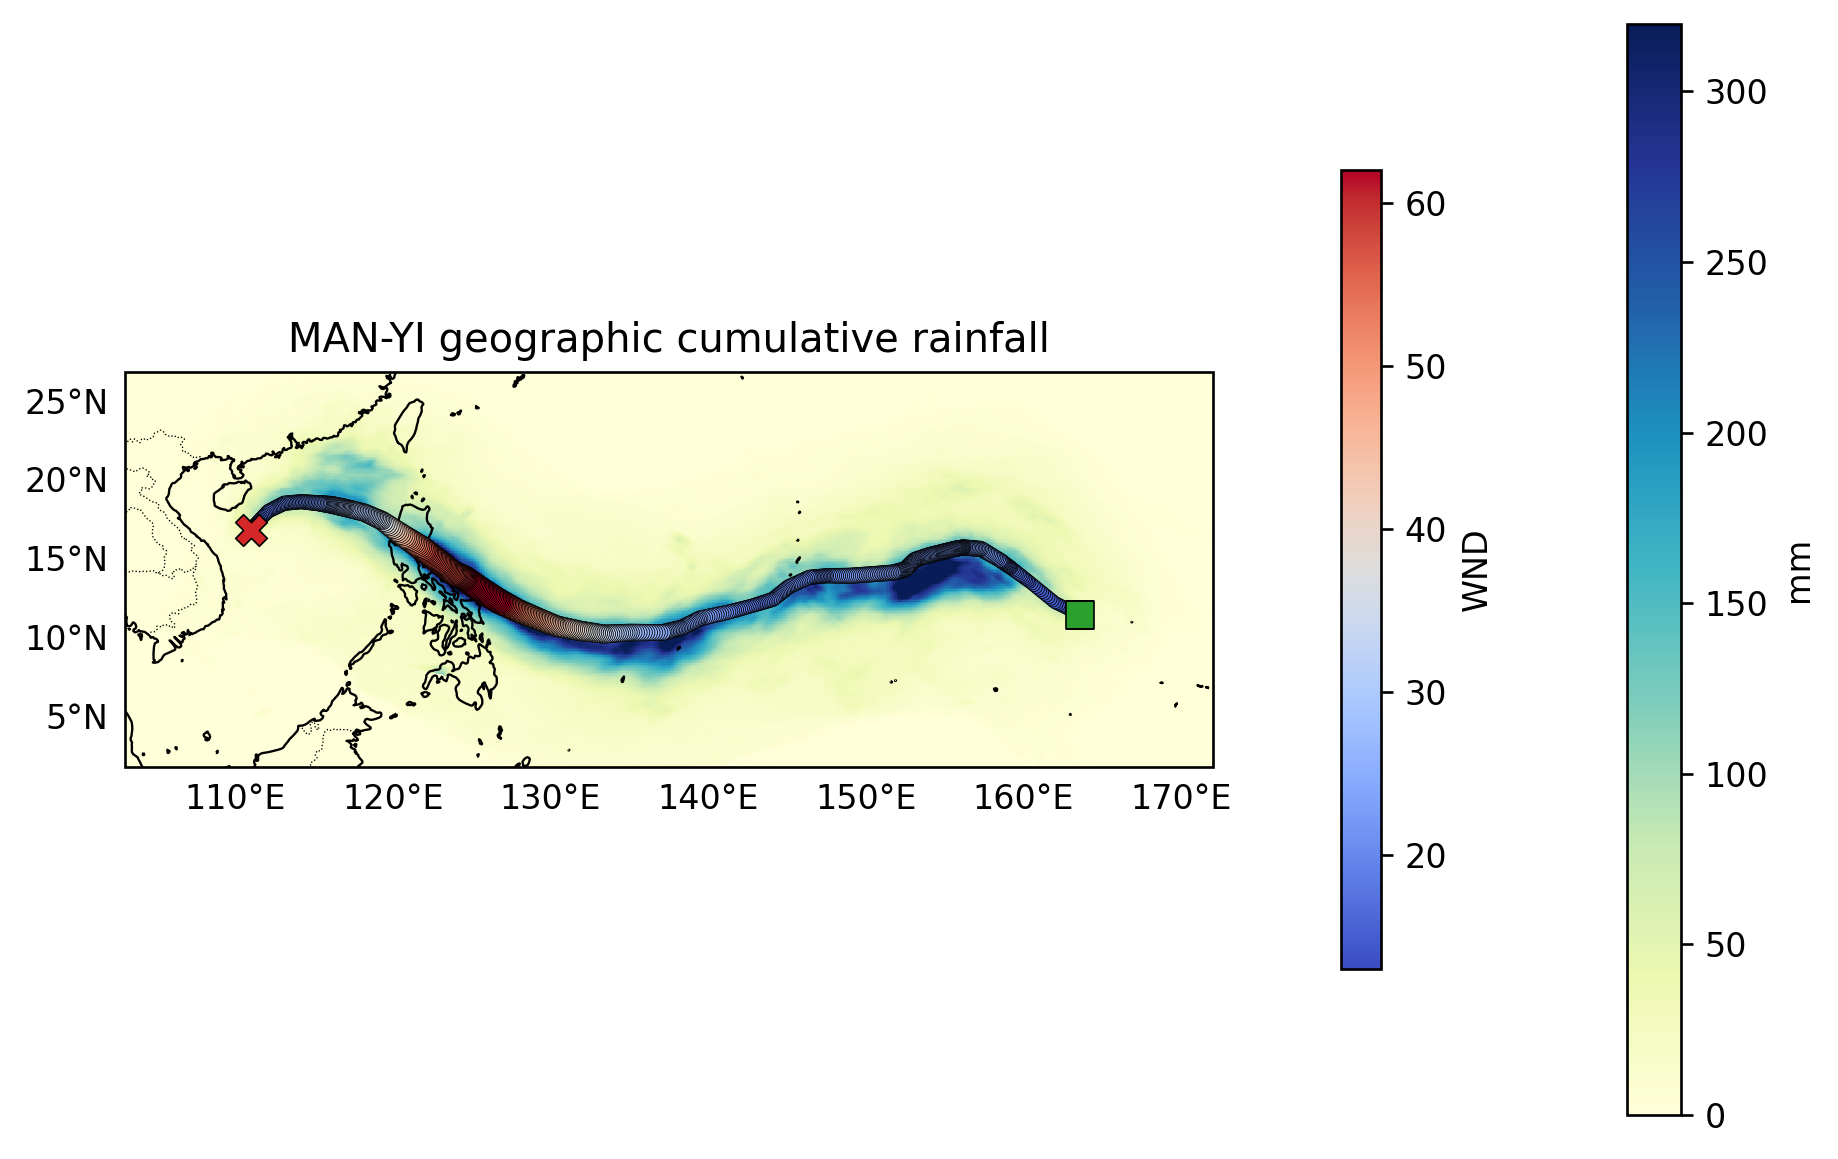
\includegraphics[width=\textwidth]{outputs/figures/problem2_geographic_results/MAN_YI_final_cumulative_rain_geographic.png}
\caption{MAN-YI 地理累计降水}
\end{subfigure}
\caption{两场台风真实地理坐标下的累计降水分布}
\label{fig:p2_geo_cum_rain}
\end{figure}

图 \ref{fig:p2_geo_max_rain} 展示了真实地理坐标下的最大半小时降水强度。KONG-REY 的最大地理半小时雨强为 $51.173\ \mathrm{mm/hr}$，发生于 2024-10-27 00:00:00，位置为 $132.2^\circ\mathrm{E}$、$15.2^\circ\mathrm{N}$；MAN-YI 的最大地理半小时雨强为 $53.529\ \mathrm{mm/hr}$，发生于 2024-11-14 10:00:00，位置为 $135.4^\circ\mathrm{E}$、$9.7^\circ\mathrm{N}$。从最大半小时雨强看，两场台风量级接近，MAN-YI 略高。

\begin{figure}[H]
\centering
\begin{subfigure}{0.48\textwidth}
\centering
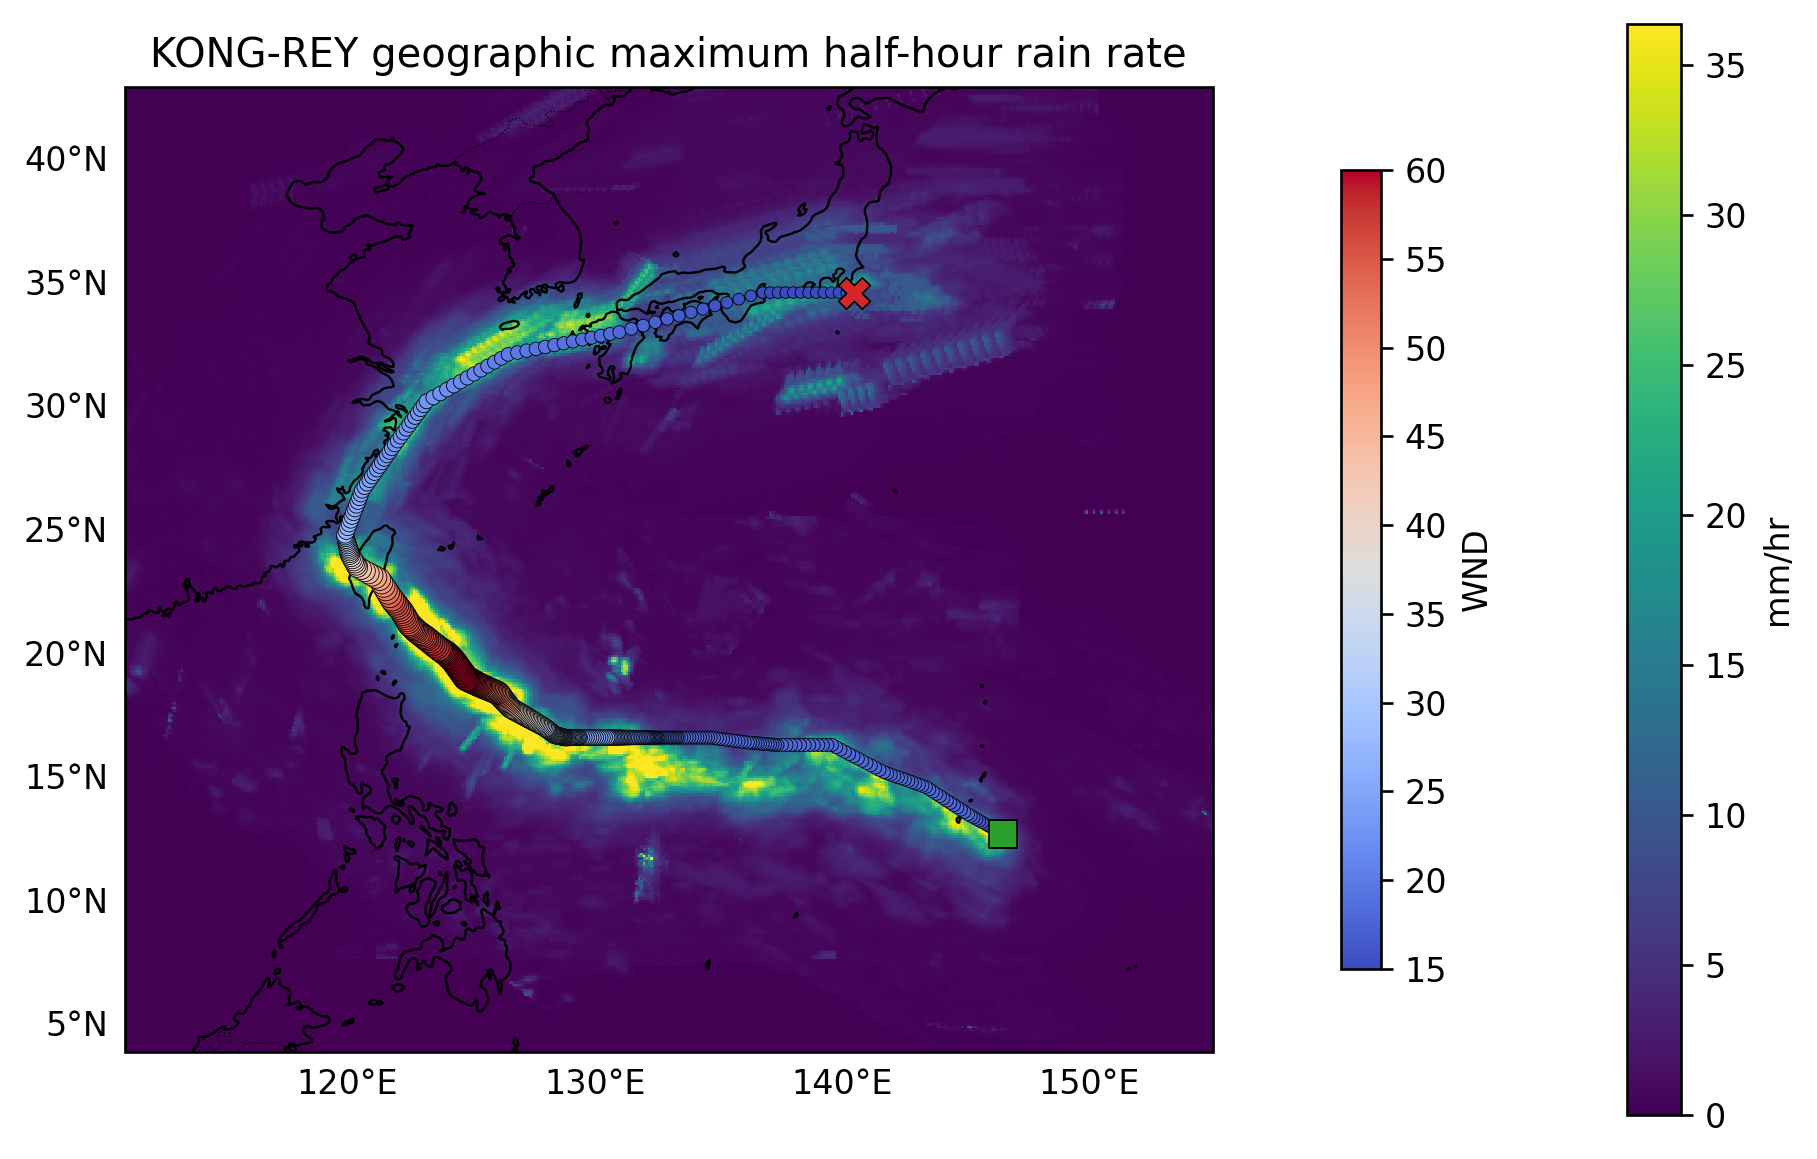
\includegraphics[width=\textwidth]{outputs/figures/problem2_geographic_results/KONG_REY_final_max_rain_geographic.png}
\caption{KONG-REY 地理最大半小时降水}
\end{subfigure}
\begin{subfigure}{0.48\textwidth}
\centering
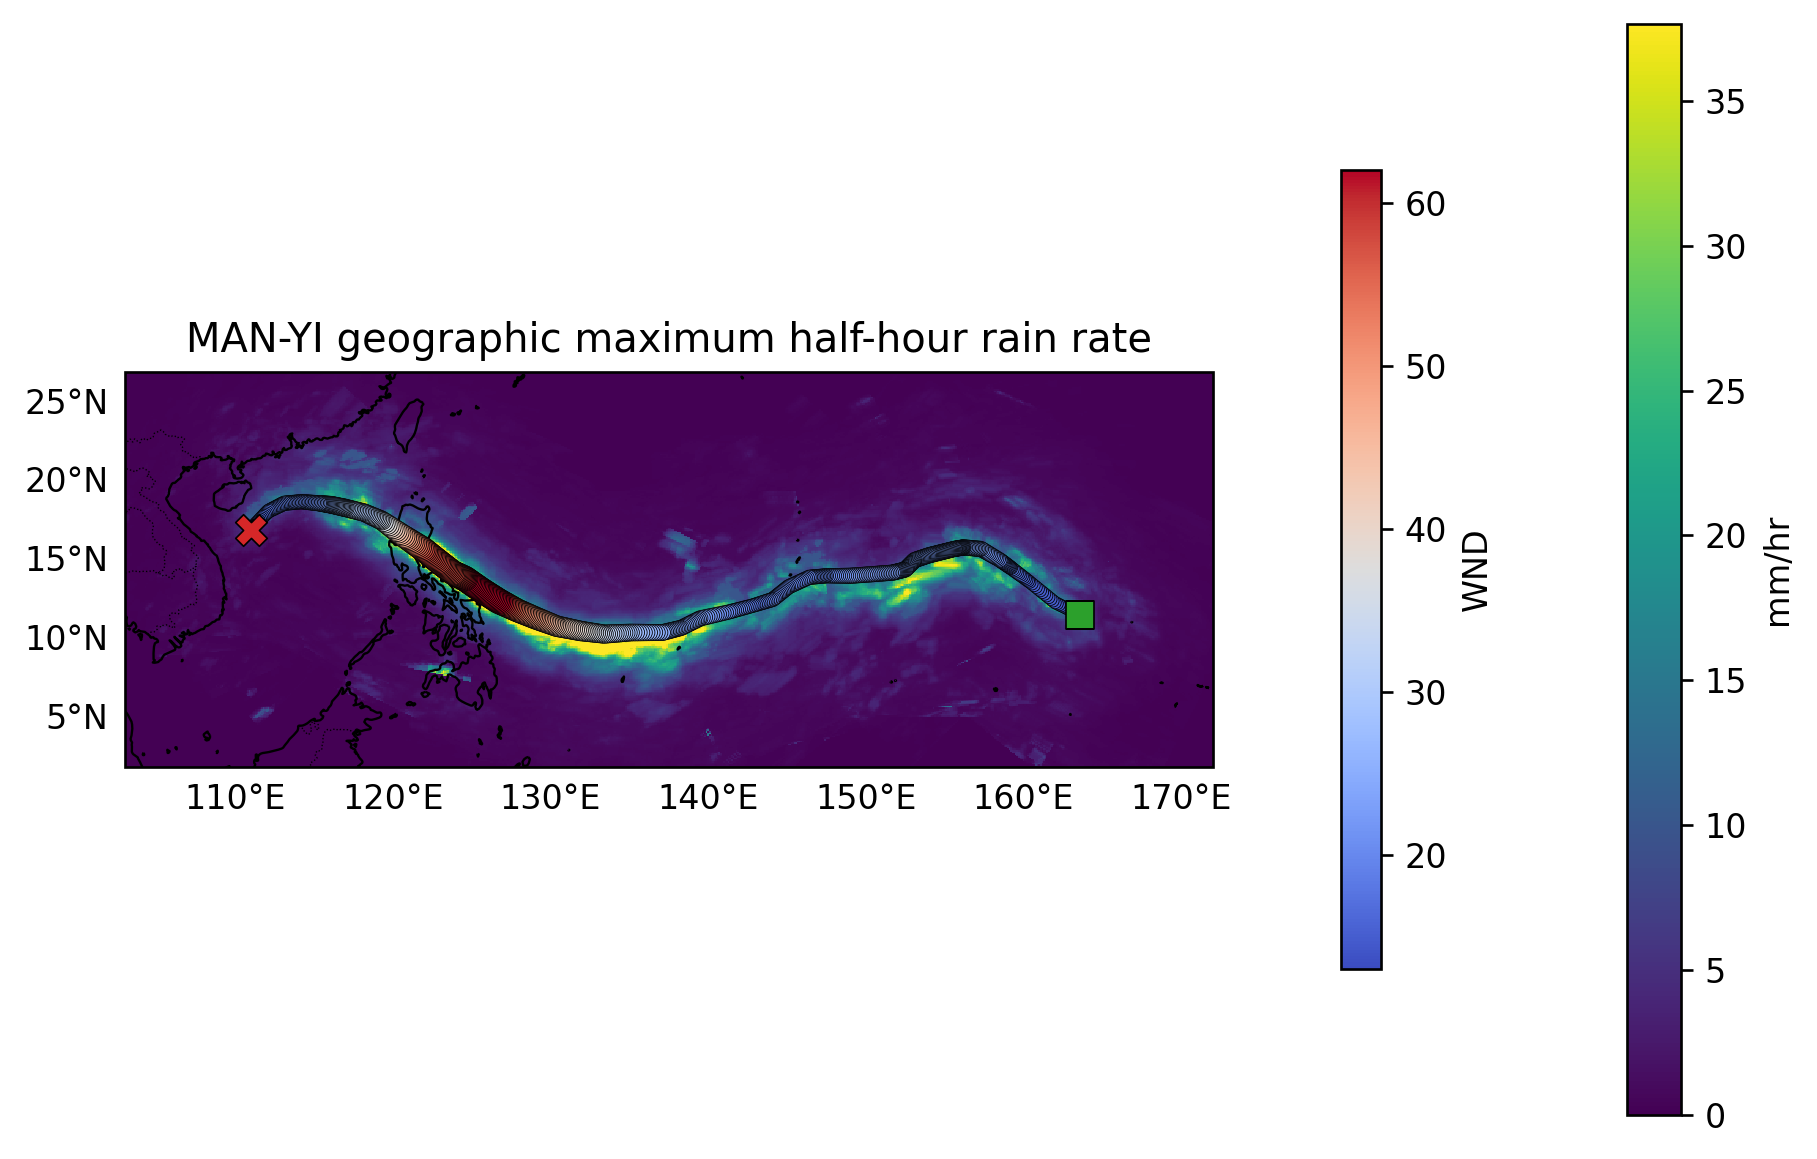
\includegraphics[width=\textwidth]{outputs/figures/problem2_geographic_results/MAN_YI_final_max_rain_geographic.png}
\caption{MAN-YI 地理最大半小时降水}
\end{subfigure}
\caption{两场台风真实地理坐标下的最大半小时降水强度分布}
\label{fig:p2_geo_max_rain}
\end{figure}

图 \ref{fig:p2_geo_duration10} 给出了 $10\ \mathrm{mm/hr}$ 阈值下的地理强降水持续时间分布。KONG-REY 的固定地理位置最大强降水持续时间为 $27.0\ \mathrm{h}$，位置为 $131.1^\circ\mathrm{E}$、$15.5^\circ\mathrm{N}$；MAN-YI 的固定地理位置最大强降水持续时间为 $23.5\ \mathrm{h}$，位置为 $153.1^\circ\mathrm{E}$、$13.8^\circ\mathrm{N}$。从单点最大持续时间看，KONG-REY 略高；但从影响范围看，MAN-YI 的 $D_{10,\mathrm{geo}}\ge3\ \mathrm{h}$ 面积达到 $1.307\times 10^6\ \mathrm{km^2}$，高于 KONG-REY 的 $8.055\times 10^5\ \mathrm{km^2}$，说明 MAN-YI 的强降水持续影响范围更广。

\begin{figure}[H]
\centering
\begin{subfigure}{0.48\textwidth}
\centering
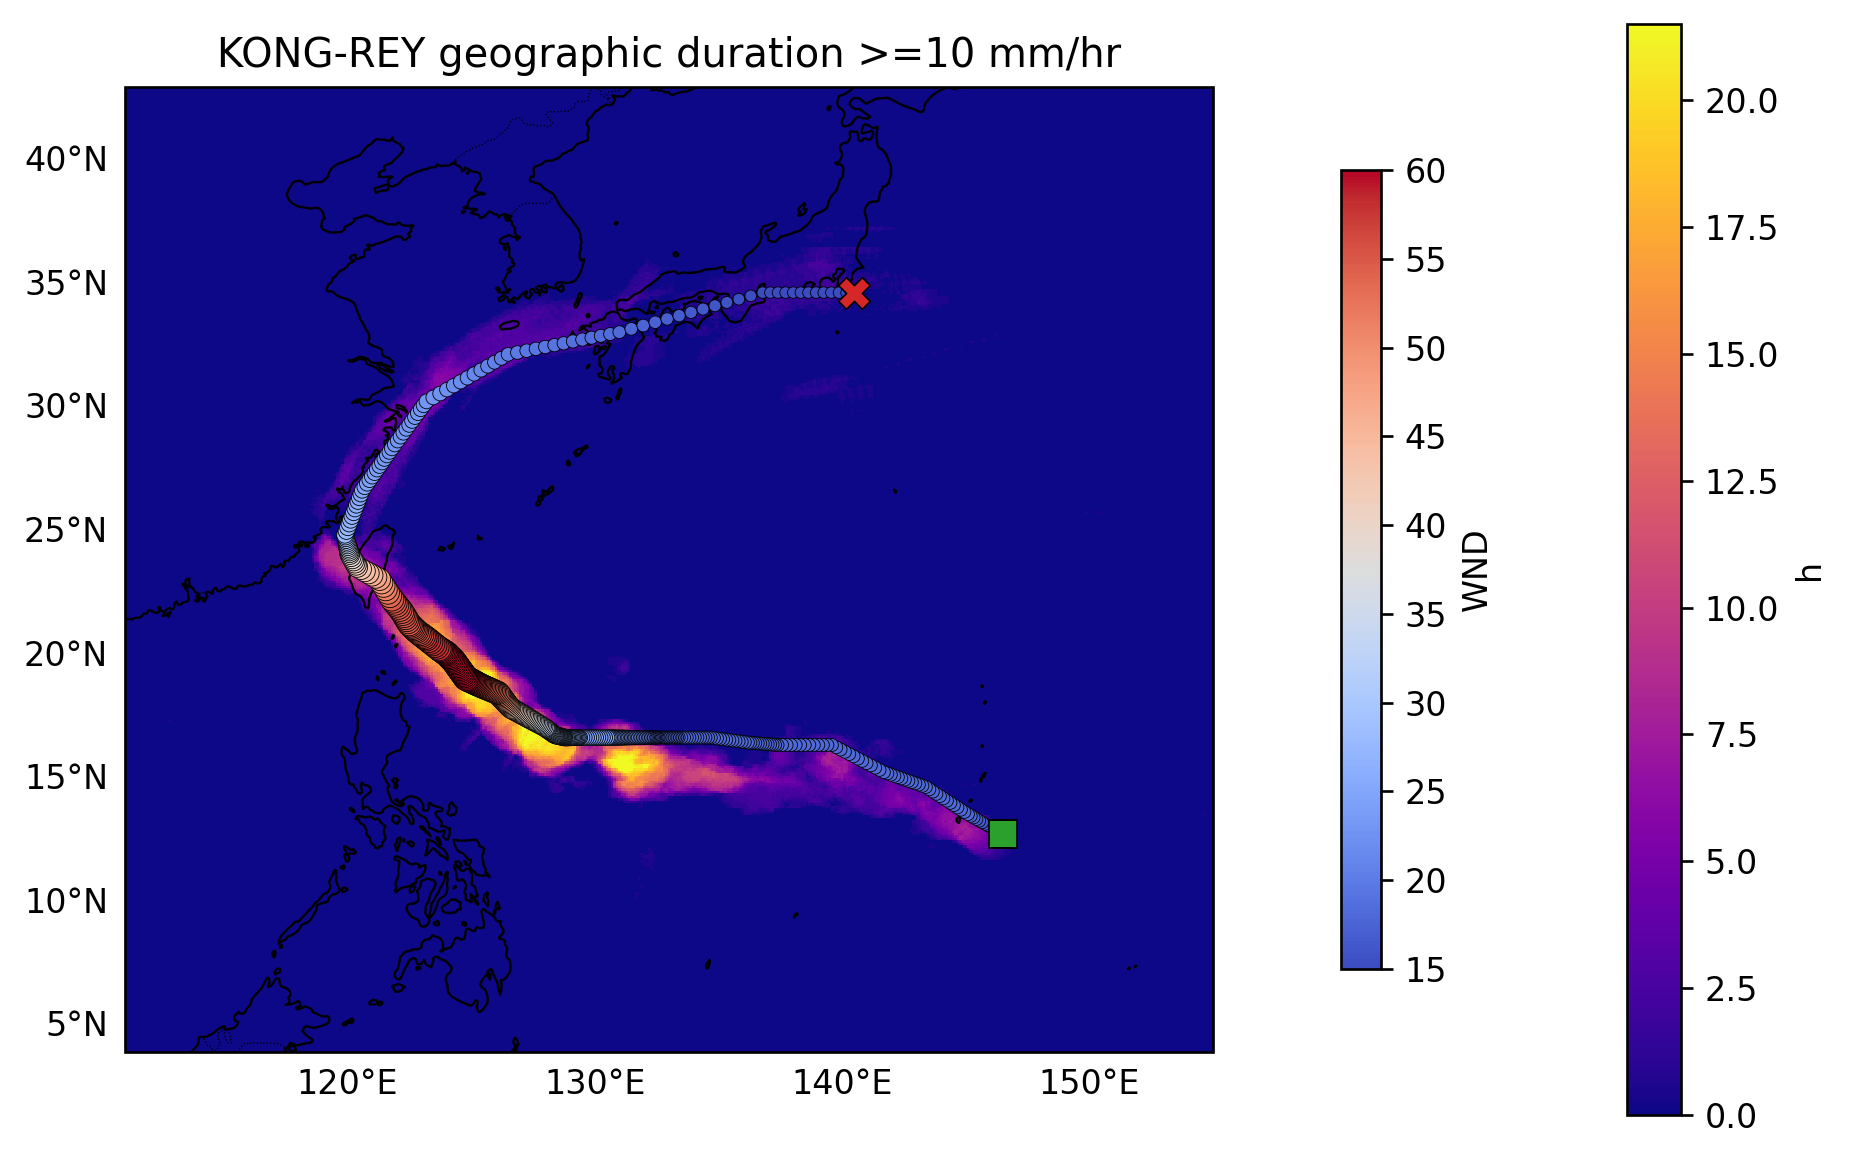
\includegraphics[width=\textwidth]{outputs/figures/problem2_geographic_results/KONG_REY_final_duration10_geographic.png}
\caption{KONG-REY 地理强降水持续时间}
\end{subfigure}
\begin{subfigure}{0.48\textwidth}
\centering
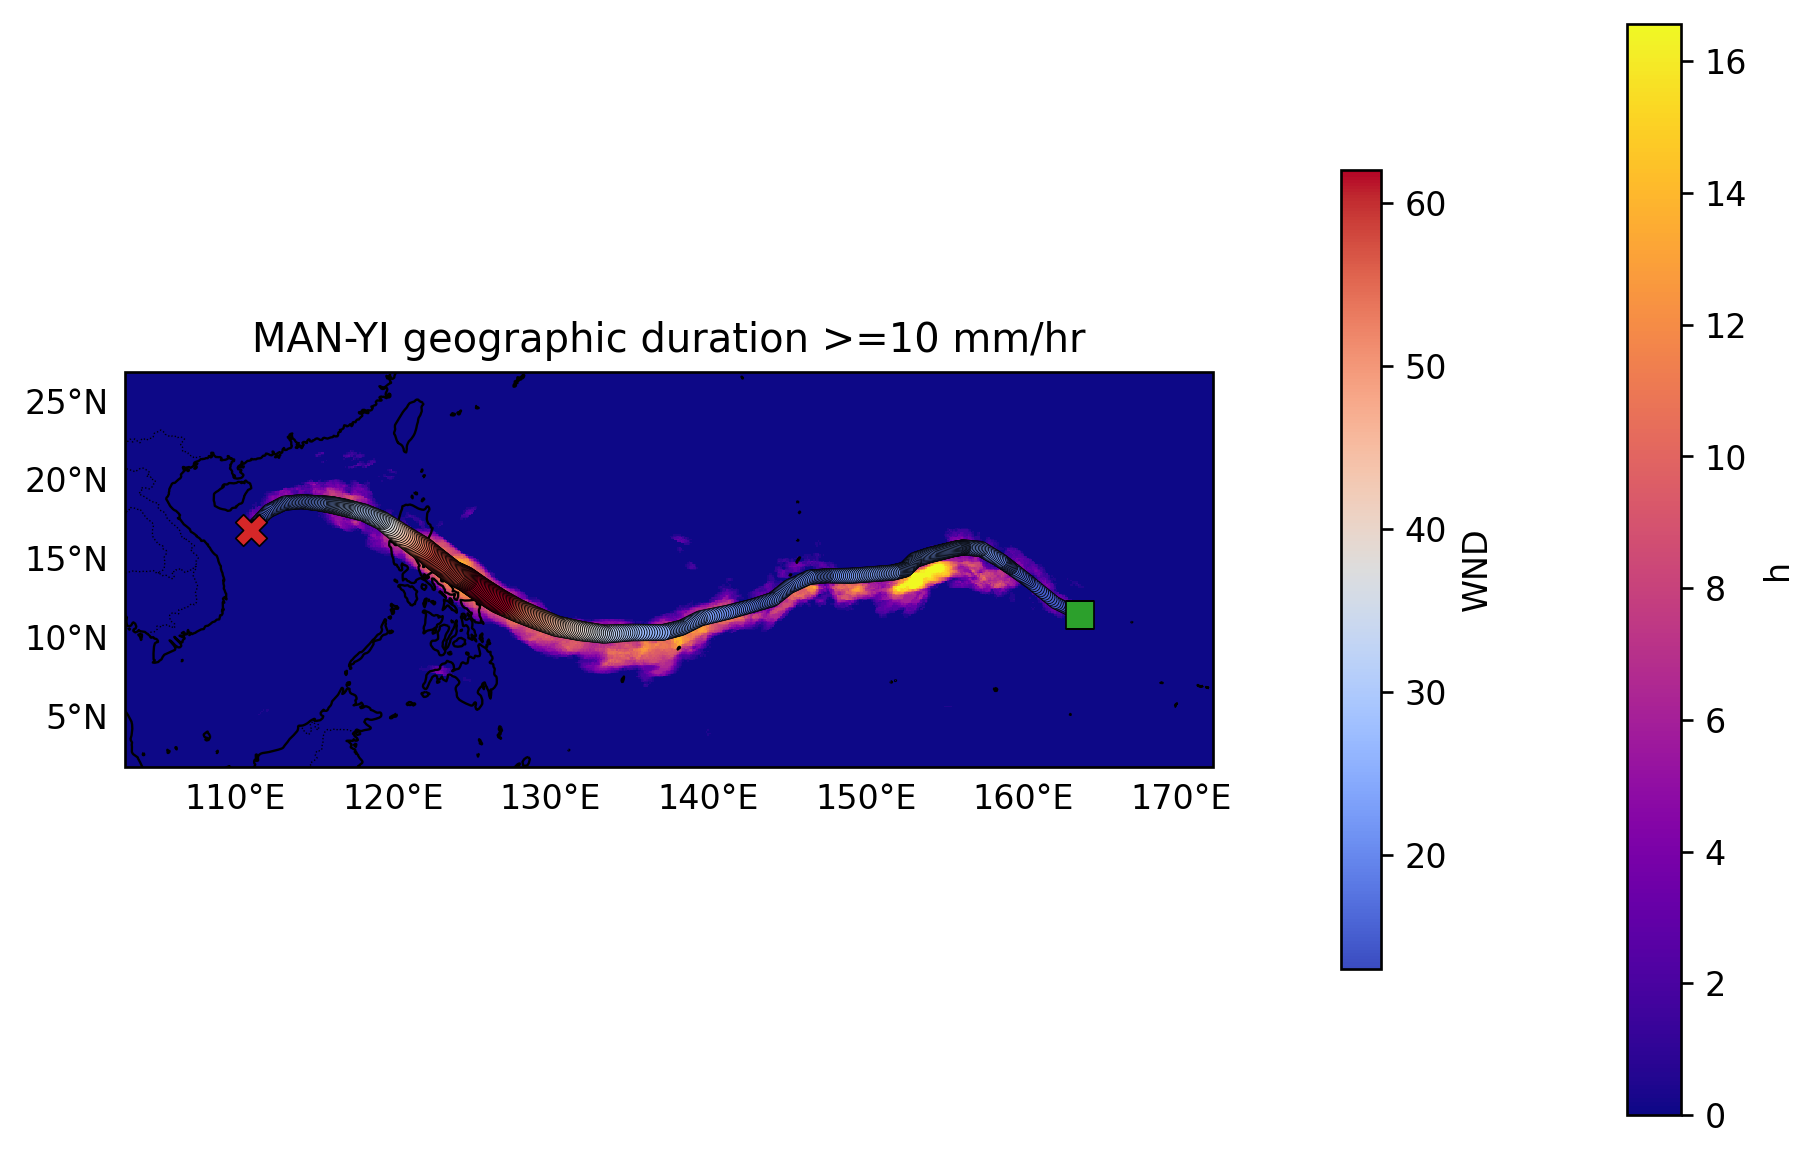
\includegraphics[width=\textwidth]{outputs/figures/problem2_geographic_results/MAN_YI_final_duration10_geographic.png}
\caption{MAN-YI 地理强降水持续时间}
\end{subfigure}
\caption{$10\ \mathrm{mm/hr}$ 阈值下两场台风真实地理强降水持续时间分布}
\label{fig:p2_geo_duration10}
\end{figure}

综合地理反投影结果可知，KONG-REY 的局地累计降水峰值更高，其最大累计降水点出现在 $124.9^\circ\mathrm{E}$、$18.6^\circ\mathrm{N}$ 附近；MAN-YI 的地理影响范围更广，其累计降水超过 $100\ \mathrm{mm}$ 的面积为 $2.071\times 10^6\ \mathrm{km^2}$，高于 KONG-REY 的 $1.229\times 10^6\ \mathrm{km^2}$。因此，从局地极端累计量看，KONG-REY 更突出；从大范围持续强降水影响看，MAN-YI 更突出。

至此，本文同时给出了两类结果：一类是台风相对坐标下的降水结构图，用于解释降水相对于台风中心和移动方向的非对称组织；另一类是真实地理坐标下的降水落区图，用于回答固定经纬度区域的可能累计降水、最大半小时雨强和强降水持续时间。二者共同构成 KONG-REY 与 MAN-YI 可能降水时空分布的最终展示。

综上，问题二所建模型在不使用目标台风真实降水记录的前提下，依据历史相似台风的路径、强度、移动和海陆环境条件，生成了 KONG-REY 与 MAN-YI 的半小时降水时空分布。伪缺失验证表明，极端校准后的模型显著提高了 P95、P99 和强降水面积的恢复能力，因此本文将 calibrated 场作为两场台风的最终可能降水分布结果。

\section{问题三模型建立与求解}

\subsection{模型改进动机}
问题三相较问题二新增了\todo{新增约束、极端场景或改进目标}。若直接使用前述模型，可能出现\todo{偏差、失效、不稳定、无法解释等问题}。因此，本文引入\todo{改进方法}。

\subsection{改进模型建立}
\begin{align}
  F_{\mathrm{new}} &= F_{\mathrm{base}} + \alpha F_{\mathrm{penalty}} + \beta F_{\mathrm{risk}}, \\
  \alpha,\beta &\geq 0 .
\end{align}
其中，$F_{\mathrm{base}}$ 表示\todo{基础目标}，$F_{\mathrm{penalty}}$ 表示\todo{惩罚项}，$F_{\mathrm{risk}}$ 表示\todo{风险或不确定性项}。

\subsection{情景设置 / 对比实验}
\begin{table}[H]
  \centering
  \caption{问题三情景设置或对比方案}
  \begin{tabular}{lccc}
    \toprule
    方案 & 关键参数 & 预期作用 & 是否采用 \\
    \midrule
    基础模型 & \todo{参数} & \todo{作用} & 是 \\
    改进模型1 & \todo{参数} & \todo{作用} & 是 \\
    改进模型2 & \todo{参数} & \todo{作用} & 可选 \\
    \bottomrule
  \end{tabular}
\end{table}

\subsection{结果与分析}
给出问题三必须提交的最终结果，并解释改进效果。
\begin{table}[H]
  \centering
  \caption{问题三核心结果}
  \begin{tabularx}{\linewidth}{lXXX}
    \toprule
    模型 / 情景 & 指标1 & 指标2 & 结论 \\
    \midrule
    基础模型 & \todo{数值} & \todo{数值} & \todo{结论} \\
    改进模型 & \todo{数值} & \todo{数值} & \todo{结论} \\
    \bottomrule
  \end{tabularx}
\end{table}

由表中结果可知，改进模型在\todo{关键指标}上提升了\todo{数值或比例}，说明\todo{回到题目要求解释}。

\section{问题四模型建立与求解（如无第四问可删除）}

\subsection{模型目标}
本问目标为\todo{策略建议 / 财务评估 / 风险预测 / 防控方案 / 决策排序}。在前三问结果基础上，构建\todo{模型或评价函数}。

\subsection{模型建立与求解}
\begin{align}
  S_k = w_1 I_{k1} + w_2 I_{k2} + \cdots + w_p I_{kp}, \quad k=1,2,\dots,K,
\end{align}
其中，$S_k$ 为第 $k$ 个方案的综合得分，$I_{kp}$ 为指标值，$w_p$ 为权重。

\subsection{结果与建议}
\begin{table}[H]
  \centering
  \caption{方案评价与建议}
  \begin{tabularx}{\linewidth}{lXXX}
    \toprule
    方案 & 优点 & 风险 & 是否推荐 \\
    \midrule
    方案一 & \todo{优点} & \todo{风险} & \todo{推荐程度} \\
    方案二 & \todo{优点} & \todo{风险} & \todo{推荐程度} \\
    \bottomrule
  \end{tabularx}
\end{table}

综合比较后，本文建议优先采用\todo{方案名称}，原因是\todo{数值依据 + 实际解释}。

\section{模型检验与灵敏度分析}

% 高分论文通常不能缺少模型检验。至少选择一种：误差分析、对比实验、交叉验证、灵敏度分析、消融实验、鲁棒性检验。
\subsection{模型有效性检验}
采用\todo{检验方法}对模型结果进行验证。评价指标定义如下：
\begin{align}
  \mathrm{RMSE} &= \sqrt{\frac{1}{N}\sum_{i=1}^{N}(y_i-\hat{y}_i)^2}, \\
  R^2 &= 1-\frac{\sum_{i=1}^{N}(y_i-\hat{y}_i)^2}{\sum_{i=1}^{N}(y_i-\bar{y})^2} .
\end{align}
若为分类问题，可改为准确率、精确率、召回率、F1 值、混淆矩阵；若为优化问题，可改为目标函数值、约束满足率、冗余率、成本变化率等。

\subsection{对比实验 / 消融分析}
\begin{table}[H]
  \centering
  \caption{模型对比结果}
  \begin{tabular}{lcccc}
    \toprule
    模型 & 指标1 & 指标2 & 指标3 & 结论 \\
    \midrule
    模型A & \todo{数值} & \todo{数值} & \todo{数值} & \todo{结论} \\
    模型B & \todo{数值} & \todo{数值} & \todo{数值} & \todo{结论} \\
    本文模型 & \todo{数值} & \todo{数值} & \todo{数值} & \todo{结论} \\
    \bottomrule
  \end{tabular}
\end{table}

\subsection{灵敏度分析}
选择关键参数 $\theta$，分别施加 $-10\%,-5\%,+5\%,+10\%$ 扰动，观察目标变量变化：
\begin{align}
  \eta = \frac{\Delta Y / Y}{\Delta \theta / \theta} .
\end{align}
当 $|\eta|$ 较大时，说明模型输出对该参数敏感，应在实际应用中重点控制或精确测量。

\begin{table}[H]
  \centering
  \caption{关键参数灵敏度分析}
  \begin{tabular}{lcccc}
    \toprule
    参数 & $-10\%$ & $-5\%$ & $+5\%$ & $+10\%$ \\
    \midrule
    $\theta_1$ & \todo{结果} & \todo{结果} & \todo{结果} & \todo{结果} \\
    $\theta_2$ & \todo{结果} & \todo{结果} & \todo{结果} & \todo{结果} \\
    \bottomrule
  \end{tabular}
\end{table}

\section{结论与最终答案汇总}

本节直接回答题目所有要求，适合放最终分类表、最优方案表、预测结果表、策略建议表等。评委应能在本节快速找到“题目问什么，本文答什么”。

\begin{table}[H]
  \centering
  \caption{各问题最终答案汇总}
  \begin{tabularx}{\linewidth}{lXX}
    \toprule
    问题 & 最终结果 & 说明 \\
    \midrule
    问题一 & \todo{结果} & \todo{说明} \\
    问题二 & \todo{结果} & \todo{说明} \\
    问题三 & \todo{结果} & \todo{说明} \\
    问题四 & \todo{若无则删除} & \todo{说明} \\
    \bottomrule
  \end{tabularx}
\end{table}

\section{模型评价与改进方向}

\subsection{模型优点}
\begin{itemize}
  \item \textbf{结构完整：}\todo{说明模型链条如何覆盖题目所有问题}。
  \item \textbf{解释性强：}\todo{说明变量、参数、结果均有实际含义}。
  \item \textbf{结果可靠：}\todo{说明进行了哪些检验}。
\end{itemize}

\subsection{模型不足}
\begin{itemize}
  \item \todo{数据量、假设简化、参数来源、计算复杂度、泛化能力等不足}。
  \item \todo{说明不足对结果可能造成的影响，不要泛泛而谈}。
\end{itemize}

\subsection{改进方向}
未来可以从\todo{更多数据、更精细模型、更高分辨率、更强验证、更贴近实际约束等}方面改进。

\section*{参考文献}
\addcontentsline{toc}{section}{参考文献}
% 正文引用格式示例：文献表明该方法适合处理非线性分类问题[1]。
% 参考文献按正文出现顺序排列。书籍需写页码；网页需写访问时间。
\begin{thebibliography}{99}
  \bibitem{ref1} 作者. 书名. 出版地：出版社，出版年：页码.
  \bibitem{ref2} 作者. 论文名. 期刊名，卷号(期号)：起止页码，出版年.
  \bibitem{ref3} 作者或机构. 资源标题. URL，访问时间：YYYY-MM-DD.
\end{thebibliography}

\appendix

\section{支撑材料文件列表}
% 支撑文件压缩包内文件名不能出现学校、姓名、队员信息。
\begin{table}[H]
  \centering
  \caption{支撑材料文件列表}
  \begin{tabularx}{\linewidth}{lXX}
    \toprule
    文件名 & 内容说明 & 对应正文位置 \\
    \midrule
    \texttt{code/main.py} & 主程序，完成\todo{模型训练 / 求解 / 仿真} & 第\todo{}节 \\
    \texttt{code/utils.py} & 数据预处理与指标计算函数 & 第\todo{}节 \\
    \texttt{data/processed.xlsx} & 清洗后的中间数据 & 第\todo{}节 \\
    \texttt{figures/workflow.pdf} & 全文流程图 & 第\todo{}节 \\
    \texttt{results/result\_table.xlsx} & 最终结果表 & 第\todo{}节 \\
    \bottomrule
  \end{tabularx}
\end{table}

若确实没有支撑材料文件，应在此处明确写明：\textbf{本论文没有支撑材料。}

\section{源程序代码说明}
% 竞赛规范要求提供完整、可运行的源程序代码。若代码过长，可在此列出核心代码结构，并在支撑材料中提供全部代码文件。
本文使用的软件环境如下：
\begin{itemize}
  \item 操作系统：\todo{Windows / macOS / Linux，不写个人路径}；
  \item 编程语言：\todo{Python 3.x / MATLAB / R / Excel 等}；
  \item 主要库：\todo{numpy, pandas, scipy, sklearn, matplotlib 等}；
  \item 运行方式：\todo{例如 python code/main.py}。
\end{itemize}

\begin{lstlisting}[language=Python,caption={核心程序框架示例，正式提交时替换为完整可运行代码}]
import numpy as np
import pandas as pd


def preprocess(raw_path: str) -> pd.DataFrame:
    data = pd.read_excel(raw_path)
    # TODO: clean missing values, outliers, and units
    return data


def solve_model(data: pd.DataFrame):
    # TODO: build and solve the mathematical model
    result = {}
    return result


if __name__ == "__main__":
    data = preprocess("data/input.xlsx")
    result = solve_model(data)
    print(result)
\end{lstlisting}

若确实没有用到程序，应在此处明确写明：\textbf{本论文没有用到程序。}

\section{人工智能工具使用说明}
% 如竞赛要求说明 AI 使用情况，可使用本节。务必如实、具体，不要写成“AI 代写论文”。
本文在\todo{建模思路梳理、代码调试、LaTeX 排版、语言润色、文献检索线索整理等}环节中使用了人工智能工具辅助。具体使用方式如下：
\begin{enumerate}
  \item 用于\todo{例如：检查摘要是否覆盖每一问的方法和结果}；
  \item 用于\todo{例如：辅助生成 LaTeX 表格框架和图表排版代码}；
  \item 用于\todo{例如：辅助解释报错信息，但最终代码由团队核查并运行验证}。
\end{enumerate}
所有模型选择、参数设定、计算结果、文字结论和参考文献均由团队成员核验。若附录需要提供使用过程截图，可在支撑材料中加入相应文件并在支撑材料列表中注明。

\section{题目要求附表（如有）}
% 若题目要求在论文附录中填写指定表格，可复制到此处。
\begin{table}[H]
  \centering
  \caption{题目要求附表模板}
  \begin{tabular}{cc}
    \toprule
    编号 & 结果 \\
    \midrule
    1 & \todo{结果} \\
    2 & \todo{结果} \\
    3 & \todo{结果} \\
    \bottomrule
  \end{tabular}
\end{table}

\end{document}
